\documentclass[a4paper, 12pt]{article}
\usepackage[brazil]{babel}
\usepackage[a4paper, inner=3cm, outer=2cm, top=3cm, bottom=2cm]{geometry}
\usepackage{charter} % fonte utilizada no documento
                    %\usepackage[nf]{coelacanth}% fontes alternativas
                    %\usepackage[T1]{fontenc} % fontes alternativas
\usepackage[utf8]{inputenc} % indicação de caracteres especiais - contidos no pt
\usepackage{microtype} %server para formatação de espaçamento e indentação
\usepackage{graphicx} % pacote de formatação e inserção de figuras
\usepackage{wrapfig} % pacote de formatação e inserção de figuras
%\usepackage{enumitem} % pacote de formatação e inserção listas enumeradas
\usepackage{fancyhdr} % pacote de formatação e inserção de cabeçalho e rodapé
\usepackage{amsmath} % pacote de formatação e inserção de equações
\usepackage{float} % pacote de formatação de tabelas e figuras
%\usepackage{index} % pacote de formatação de sumário
\usepackage{booktabs} % pacote de formatação e inserção de tabelas
\usepackage{hyperref} % pacote para uso de hyperlinks
%\usepackage{abntex2cite} % Citações padrão ABNT
\usepackage[style=abnt, sorting=ynt]{biblatex} % formatação e configuração das referências
\addbibresource{ref.bib}
\usepackage{csquotes}
\usepackage[at]{easylist} % pacote mais fácil pra editar listas e enumerações
\usepackage[singlespacing]{setspace} % pacote de formatação de espaçamento entre linhas
%\usepackage{blindtext} % pacote de inserção de texto randomizado - lorem ipsum

%-------cabeçalho e rodapé-------%
\pagestyle{fancy} % estilo do cabeçalho e rodapé
\fancyhf{}
\rhead{FRAGA, Anderson A.}
\lhead{Zero Energy para Edifícios Comerciais em Vitória-ES}
\rfoot{Página \thepage}
\renewcommand{\headrulewidth}{2pt}
\renewcommand{\footrulewidth}{1pt}
\setlength{\headheight}{15pt} % formatando o headheight, eliminamos o conflito com o pacote fancyhdr
%\setlenght{\parindent}{1.3cm}
%\setlenght{\parskip}{0.2cm}

%-------início da dissertação-------%
\begin{document} %capas
\begin{titlepage}
    \begin{center}
        \begin{figure}
            \centering
            
\includegraphics[scale=1.15]{F:/Root Files/Academic/masters/_desenvolvimento/_regular/_dissertacao/fase final/_estrutura/_texto/tex/figures/brasao-rep-br.png}
        \end{figure}
        \vspace*{0.1cm}
        \textbf{\large Universidade Federal do Espírito Santo}\\
        \large Centro de Artes\\
        \large Programa de Pós-Graduação em Arquitetura e Urbanismo\\
        \vspace*{3cm}
        \textbf{\large Anderson Azevedo Fraga}\\
        \vspace*{4cm}
        \textbf{Potencial de Adoção do Conceito Zero Energy para Edifícios Comerciais em Vitória-ES}\\
        \vfill % preenche em branco o espaço até o final da página
        Vitória\\
        2020

    \end{center}
\end{titlepage}

%\title{Potencial de Adoção do Conceito Zero Energy para Edifícios Comerciais 
%em Vitória-ES}
%\author{Anderson Azevedo Fraga}
%\date{Setembro de 2020}

\thispagestyle{empty} % limpa cabeçalho, rodapé e número de página
\pagebreak

\section*{Resumo}
    \vspace*{1.5cm} % verificar se é permitido manter este espaçamento
    \thispagestyle{empty}
    \begin{onehalfspace}
        O consumo de energia no uso de edificações vem crescendo gradativamente ao longo 
    das últimas décadas, fruto do desenvolvimento industrial e da revolução tecnológica 
    que vem acompanhando este movimento. A emissão de gases poluentes e a modificação 
    do clima são consequências desse cenário de desenvolvimento e consumo. 
    Aliado a esses fatores, as edificações contribuem para o agravamento  desse  cenário,  
    uma  vez  que  o  uso  destas  acarreta  em  impactos  negativos significativos ao 
    meio ambiente. Em contraponto, edificações energeticamente eficientes vêm se tornando  
    pré-requisito  para  o  planejamento  de  novos  ambientes  construídos,  modificando  
    a forma  como  a  comunidade  percebe  a  relação entre a edificação  e  o  consumo de  
    energia.  Este trabalho  tem  como  objetivo  estudar  o  potencial  de  aplicação  
    do  conceito Zero Energy  para edificações comerciais, com o intuito de verificar a validade 
    do método para o cenário construtivo brasileiro adotando como estudo de caso  uma 
    edificação  em Vitória (ES). Metodologicamente, este  estudo  foi  desenvolvido  com  
    base  em  três  grandes  etapas,  onde  a  primeira  consistiu  em realizar  o  
    levantamento  das  edificações  dentro  de  um  recorte  territorial  pré-estabelecido, 
    selecionar as características construtivas e arquitetônicas mais frequentes entre elas e 
    construir modelos  representativos  do  cenário  observado;  a  segunda  consistiu  
    em  submeter  os  modelos representativos à simulações computacionais para avaliar o 
    desempenho energético, as possíveis formas  de  eficientização  e  de  produção  de  
    energia;  e  por  fim,  a  terceira  etapa,  na  qual  foi realizada  avaliação  dos  
    resultados  e  da  viabilidade  econômica  de  implantação  do  sistema  de produção 
    de energia. Os resultados mostraram que as estratégias de implementação de sistemas de 
    condicionamento de ar, de equipamentos e iluminação mais eficientes são muito importantes 
    para  a  economia  de  energia.  É  perceptível  que  a  proposição  de  soluções  
    construtivas  e arquitetônicas  mais  eficientes  em  relação  ao  desempenho  energético  
    associado  a  técnicas  de obtenção  de  energia  podem  resultar  em  uma  edificação  
    com  o  balanço  energético  nulo  ou próximo ao nulo. Esses resultados indicam que a adoção 
    desse conceito para novas edificações é factível e cada vez mais acessível à comunidade.\\
    
    \noindent Palavras-chave: zero energy buildings; balanço energético nulo; edifício de escritório.\pagebreak
    \end{onehalfspace} % preâmbulo e listas
\section*{Abstract}
    The  energy  consumption  in  using  a  building  is  growing  in  constant
    pace  in  the  last  decades, coming from the industrial development and 
    technological revolution which comes together with this movement. 
    The emission of Greenhouse Gas and climate change are consequences of these 
    scenario  of  development  and  consumption.  Allied  to  these  factors,  
    buildings  contribute  to  the worsening of this scenario, since the use of 
    these  constructions mean negative  impacts on  the environment.  In  contrast,  
    energy  efficient  buildings  have  become  a  must-do  for  planning  
    new built  environments,  changing  the  way  the  community  perceives  
    the  relationship  between  the building and energy consumption. This work 
    aims to study the potential application of the Zero Energy concept for commercial 
    buildings in Vitória, in order to verify the validity of the method for the 
    Brazilian construction scenario and contribute to the dissemination of this 
    form of building planning. Therefore, this study was developed based on three 
    major stages, as the first consisted of surveying the buildings within a 
    pre-established territorial outline, selecting the most frequent construction  
    and  architectural  characteristics  among  them  and  build  representative  
    models  of the  observed  scenario;  the  second  stage  consisted  of  subjecting  
    the  representative  models  to computer  simulations  to  show  the  energy  
    performance  of  the  buildings  surveyed,  ways  to optimize  and,  
    thus,  reduce  the  energy  consumption  of  the  models  and  forms  of  solar  
    energy production  applied  to  the  reference  buildings;  and  finally,  
    the  third  stage,  in  which  the  results were evaluated and the economic 
    feasibility of implementing the energy production system were done.  
    The  results  showed  that  the  strategies  for  implementing  more  efficient  
    air  conditioning systems,  equipment  and  lighting  are  very  important  
    for  energy  savings.  The  combination  of construction  and  architectural  
    modifications  for  materials  with  higher  energy  performance provide the 
    environment to achieve zero energy or near zero energy states. 
    These results indicate that the adoption of this way of thinking about building 
    is feasible and increasingly accessible to the community.\\

    \noindent Keywords: zero energy buildings; near zero energy buildings; office buildings.
    \pagebreak
\begin{}
    LISTA DE ABREVIATURAS
    ABIVIDRO – Associação Técnica Brasileira das Indústrias Automáticas de Vidro
    ABNT – Associação Brasileira de Normas Técnicas
    ANAEEL – Agencia Nacional de Energia Elétrica
    ARSP – Agência de Regulação de Serviços Públicos do Espírito Santo
    ASHRAE – American Society of Heating, Refrigerating and Air-conditioning Engineers
    ASPE – Agência de Serviços Públicos de Energia do Espírito Santo
    CB3E – Centro Brasileiro de Eficiência Energética em Edificações 
    CBCS – Conselho Brasileiro de Construção Sustentável 
    CNI – Confederação Nacional da Industria 
    DOE – Department of Energy of United States of America 
    EPE – Empresa de Pesquisa Energética 
    IBGE – Instituto Brasileiro de Geografia e Estatística 
    IEA – International Energy Agency 
    INCAPER – Instituto Capixaba de Pesquisa, Assistência Técnica e Extensão Rural 
    INMET – Instituto Nacional de Meteorologia 
    INMETRO – Instituto Nacional de Metrologia, Qualidade e Tecnologia 
    ONS – Operador Nacional do Sistema Elétrico 
    PMV – Prefeitura Municipal de Vitória 
    SIN – Sistema Interligado Nacional 
    SINDUSCON – Sindicato da Indústria da Construção Civil do Espírito Santo 
    UNDP – United Nations Development Programme 

\end{}
\listoffigures\pagebreak
\listoftables\pagebreak
\tableofcontents\pagebreak

\section{Introdução}
\begin{onehalfspace}
A energia elétrica é um recurso essencial para o desenvolvimento econômico de um país, para a qualidade de vida  da população e para a manutenção do meio ambiente por meio de seu uso eficiente \cite{Fonseca2016}. A importância do uso racional e eficiente deste recurso torna imprescindível a conservação e redução do seu desperdício para a sustentabilidade do ambiente em que se vive.\vspace*{0.3cm} \newline
Desde a crise do petróleo, ocorrida nos anos de 1970, a eficiência energética tem a função de proporcionar condições para suprir à demanda futura de energia. Esta gestão eficiente do consumo de energia é essencial para reduzir o impacto energético de setores como o de edificações, o qual consome de 36 a 40\% da energia total final global. A necessidade de expansão dos setores econômicos provoca demanda por energia elétrica. Esta busca resulta em desperdícios oriundos da falta de políticas públicas efetivas, de investimento em tecnologia e de fiscalização sobre o consumo deste insumo \cite{InternationalEnergyAgency-IEA2019,InternationalEnergyAgency-IEA2019a, UnitedNationsEnvironmentProgramme-UNEP2019,UnitedNations2017}.\vspace*{0.3cm} \newline
Em contraponto à demanda e ineficiência energética, as edificações comerciais, em particular as de escritório, podem desempenhar funções estratégicas como minimizar o uso energético e produzir eletricidade, aproximando ou equalizando a zero a razão entre a produção e o consumo de energia. Estas edificações são denominadas edificações com balanço energético nulo, ou \textit{Zero Energy Buildings} – ZEB \cite{Crawley2009,Torcellini2006,Kurnitski2011,Kurnitski2011a,Torcellini2015}.\vspace*{0.3cm} \newline
Calcula-se que a tendência de adoção desta forma de projetar edificações crescerá até 2050, haja vista que a publicação de normas e regulamentações acerca do tema vêm crescendo ao redor do mundo \cite{UnitedNationsEnvironmentProgramme-UNEP2019}. Com a introdução de uma ZEB, a exploração de recursos renováveis complementares como a energia solar, e a utilização de tecnologia solar fotovoltaica, surgem como opção para minimizar as consequências negativas causadas por condições climáticas, de infraestrutura e socioeconômicas adversas \cite{Pikas2014,Pikas2017}.\vspace*{0.3cm} \newline
A quantidade de radiação solar recebida no Brasil, por exemplo, alcança a ordem de 1.013 MWh, nível acima de países com grande capacidade de geração de energia solar. Este fato torna viável a adoção deste recurso como forma de reduzir o uso de fontes de energia fósseis e como economia no consumo de água. A disponibilidade de energia solar no Brasil alcança cerca de 6,5 kWh/m² ao ano e, no Espírito Santo, entre 4,8 a 5,2 kWh/m² ao ano \cite{AgenciadeRegulacaodeServicosPublicosdoEspiritoSanto-ARSP2019, Didone2014,InternationalEnergyAgency-IEA2018}.\vspace*{0.3cm} \newline
A relação entre fontes da matriz energética brasileira é composta por 45\% de fontes renováveis e 55\% de fontes não-renováveis de energia. Há, ainda, a previsão de que a parcela de geração de eletricidade por meio de fontes renováveis, que em 2018 era de 83,3\%, atinja 87\% até 2040 \cite{EmpresadePesquisaEnergetica-EPE2017}. No entanto, há controvérsias na classificação da fonte hidrelétrica como renovável, considerando a dependência da água, dos ciclos de chuva e dos impactos gerados na construção das usinas \cite{Leme2012}.\vspace*{0.3cm} \newline
Dentro  do  contexto  de  segurança  energética,  a  crise  brasileira,  ocorrida  em  2001, provocou mudanças no planejamento do fornecimento de energia elétrica, com o posterior surgimento de medidas  atenuantes  às dificuldades  de  cunho  ambiental  e  de  infraestrutura  da  época.  Em  seu ápice, no ano de 1999, o país passou pelo período popularmente denominado “apagão”, o qual representou  a  falta  de  fornecimento  em  70\%  do  território  nacional.  O  consumo  de  energia elétrica, entre os anos de 1990 e 2000, sofreu aumento de 49\%, enquanto a capacidade instalada foi expandida em 35\%, ocasionando o descompasso entre consumo e fornecimento nesta época \cite{Conejero2016,Tolmasquim2000}.\vspace*{0.3cm} \newline
Verifica-se  também  que  a  centralização  de  geração  de  energia  representa  fragilidade  para  o modelo  de  comercialização  utilizado  no  Brasil \cite{Pinto2017}. Logo,  as mudanças observadas sobre a incorporação e aumento da participação de fontes renováveis de energia  no mix  energético  brasileiro,  além  da  inserção  de  edificações  com  alto  desempenho energético como as ZEB’s, pode servir como uma das respostas necessárias visando a segurança energética  e  elevando  a  confiabilidade  do  SIN  -  Sistema  Interligado Nacional \cite{EmpresadePesquisaEnergetica-EPE2017a}.\vspace*{0.3cm} \newline
No âmbito estadual, o Espírito Santo vem apresentando redução na produção de energia limpa nos últimos 8 anos, quando comparado proporcionalmente ao consumo de fontes tradicionais. Existe ainda a parcela de geração de energia elétrica oriunda de fontes não-renováveis de energia, como usinas termelétricas, correspondendo a 65\% de toda a capacidade instalada em operação do  Espírito  Santo,  restando  35\%  de  fontes  renováveis,  composta  por  usinas  hidrelétricas,  com participação  de  34\%,  e  geradores  de  energia  solar  fotovoltaica,  com  1\% \cite{AgenciadeRegulacaodeServicosPublicosdoEspiritoSanto-ARSP2019,EnergiasdePortugal-EDP2017}.\vspace*{0.3cm} \newline
Sabe-se  que  as  edificações  comerciais no  Brasil  utilizam  majoritariamente  a  eletricidade, em especial  as  edificações  de escritório,  com  aproximadamente  92\%  do  consumo  total,  enquanto edificações  de  uso  não-comercial  utilizam  fontes  de  energia  diversificadas.  Assim,  a  redução superficial de consumo de energia destas edificações nos últimos 5 anos, quando comparado com os  outros  setores  econômicos,  é  da  ordem  de  2,74\%,  o  que  reforça  a  importância  em proporcionar  o  aumento  da  eficiência  energética  para  o  segmento  de  edificações  comerciais \cite{AgenciadeRegulacaodeServicosPublicosdoEspiritoSanto-ARSP2018, AgenciadeRegulacaodeServicosPublicosdoEspiritoSanto-ARSP2019, EmpresadePesquisaEnergetica-EPE2018}.\vspace*{0.3cm} \newline
À vista  destes dados,  a presente pesquisa objetivou avaliar  o  potencial de adoção  do  conceito \textit{Zero Energy}   enquanto   uma  das  possíveis   estratégias  visando   a   redução   dos  problemas energéticos e ambientais relacionados às edificações de escritório, como forma de contribuir aos novos mecanismos para planejar e projetar o ambiente construído. Da mesma forma, busca-se evidenciar  medidas que propiciem  a  redução  do impacto  do  consumo  energético  vinculado  ao uso destes edifícios.
\end{onehalfspace}
 % corpo da dissertação
\subsection{Questionamentos}
\begin{onehalfspace}
        Considerando que:
    \begin{itemize}
        \item Existe uma parcela de energia elétrica proveniente de fontes fósseis no 
        Estado e que este quadro pode se agravar ao longo do tempo, visto a falta de 
        representatividade das fontes alternativas de geração de energia na matriz 
        energética do Espírito Santo;
        \item A demanda energética das edificações comerciais poderia  ser reduzida,  se 
        desde a fase projetual fosse considerada as potencialidades e restrições 
        ambientais do entorno;
        \item A micro e mini geração de energia elétrica é uma possibilidade que deve ser 
        incrementada no Brasil, principalmente considerando o potencial de queda de custos 
        na implementação de fontes de geração de energia elétrica descentralizada;
        \item Os   componentes   da   edificação,   como   envoltória   e   os   sistemas   
        de   conforto termoenergético, são subutilizados ou mal dimensionados no âmbito do 
        recorte territorial considerado, acarretando a baixa eficiência energética do 
        edifício.
    \end{itemize}
    A pergunta foi estabelecida a partir do seguinte questionamento: 
    considerando as características do  ambiente  construído  no  âmbito  da  Região  
    Metropolitana  da  Grande  Vitória,  é  possível desenvolver edificações cujos valores 
    de demanda e produção de energia elétrica resultem em nulo ou quase nulo?
\end{onehalfspace}
\subsection{Objetivos}
\begin{onehalfspace}
Diante do exposto, o objetivo principal desta pesquisa foi avaliar 
a aplicabilidade do conceito \textit{Zero Energy}  em  edificações  comerciais,  
especificamente  de  escritório,  com  estudo  de  caso  para  o 
município  de  Vitória  (ES).  Este  setor  foi  selecionado  por  
apresentar  padrões  amplamente difundidos  de  uso  e  ocupação,  
de  equipamentos  e  da  conformação  do  espaço,  que  não  
só viabilizam  a  adoção  de  tecnologias  de  produção  de  energia  
elétrica,  como  também  facilita  a análise de desempenho termoenergético, 
quando comparado às edificações do setor industrial e do setor residencial.\newline
Visando alcançar os resultados esperados, foram definidos os seguintes 
objetivos específicos:
\begin{itemize}
    \item Identificar os parâmetros aplicáveis às edificações de escritório 
    inerentes ao conceito \textit{Zero Energy} e \textit{Near Zero Energy}, assim como sua 
    viabilidade econômica;
    \item Mapear e diagnosticar as edificações comerciais concluídas a partir 
    de 2003, em Vitória – ES,  como  recorte  da  pesquisa,  com  a  
    caracterização  da  envoltória  e  dos  sistemas  de iluminação e 
    condicionamento de ar;
    \item Identificar métodos para a geração energética e formas de 
    racionalização do consumo de energia, estabelecendo diretrizes para 
    situações semelhantes.
\end{itemize}
\end{onehalfspace}
\section{Referencial Teórico}
Este capítulo trata das referências utilizadas para o desenvolvimento da 
pesquisa. O referencial teórico foi organizado, em grande parte, com base 
nos estudos de Didoné (2014), Didoné, Wagner e  Pereira  (2014),  Kurnitski 
et al.  (2011)  e  Torcellini et al.  (2006).  Estas  referências  tratam  
das definições sobre Zero Energy Buildings, sobre conforto ambiental por 
meio de estratégias passivas e ativas, a eficiência energética voltada a 
edificações e a produção de energia elétrica por meio de tecnologias 
fotovoltaicas. Estes autores foram escolhidos por serem referências 
recorrentes em pesquisas posteriores as publicações citadas e apresentarem 
metodologias e embasamentos teóricos importantes para o desenvolvimento de 
pesquisas sobre o tema Zero Energy. Da mesma forma, foram utilizados 
conceitos abordados pela Instrução Normativa Inmetro para Classe de 
Eficiência Energética de Edificações Comerciais, de Serviços e Públicas 
– INI-C (2018) e pelas  normas  NBR  15.220  (2019),  e The American 
Society of Heating, Refrigerating and Air-Conditioning 
Engineers – ASHRAE Standard 55 (2017), 140 (2017) e 90.1 (2010). 
O contexto socioeconômico e climático de Vitória, assim como a caracterização 
da tipologia de referência  para  suporte  metodológico  das  simulações  
e  constituição  dos  modelos  genéricos foram abordados neste capítulo.

\subsection{Introdução ao conceito Zero Energy}
Define-se que um edifício Zero Energy – ZEB, ou em português, balanço 
energético nulo, é uma edificação  energeticamente  eficiente  onde,  
considerada  a  fonte  energética,  a  energia  elétrica fornecida pela 
concessionária é anualmente menor ou igual à quantidade de energia renovável 
exportada pela edificação para a rede 
\cite{Torcellini2006,U.S.DepartmentofEnergy-USDOE2012,U.S.DepartmentofEnergy-USDOE2015}. 
Domingos et al.  (2014)  define  que  o  balanço  energético  nulo  pressupõe  
uma  arquitetura adequada ao uso de elementos construtivos e equipamentos 
de alta eficiência energética, aliado ao desempenho da fonte geradora de 
energia elétrica a partir de fontes renováveis. A redução do consumo de 
energia em novas edificações ou em processo de melhoria pode ser alcançada 
por meio de projetos integrados à tecnologias de produção de energia, com 
adoção de soluções   energeticamente   eficientes,   e   por   programas   
de   economia   de   energia   (U.S. DEPARTMENT OF ENERGY, 2015). 
Torcellini et al. (2006) estabelecem quatro definições acerca das formas de 
se atingir o ZEB em edificações  de  baixo  consumo  de  energia,  ou  
comumente  denominadas Low-Energy Buildings. Dentre as formas estudadas estão: 
\begin{itemize}
    \item Zero Site Energy, ou energia local zero ou ainda energia da 
    edificação (U.S. DEPARTMENT OF ENERGY, 2015), onde é avaliada a 
    potencialidade de produção de energia elétrica para a  edificação  
    utilizando  os  recursos  presentes  no  local,  ou on-site,  onde  o  
    edifício  está implantado. É minimamente avaliado o consumo dos 
    sistemas de condicionamento de ar, de aquecimento quando existente, 
    ventilação, cargas de equipamentos e de sistema de iluminação;
    \item Zero Source Energy,  ou  fonte  de  energia  zero,  trata-se  do  
    conceito  onde  é  levado  em consideração toda a cadeia de produção 
    total anual de energia utilizada pela edificação e de consumo de 
    energia primária do edifício. Esta avaliação leva em conta a 
    eletricidade, combustíveis utilizados em processamento e transporte de 
    materiais e componentes para o local da edificação, entre outros aspectos;
    \item Zero Energy Cost, ou custo de energia zero, é avaliada a razão, 
    no mínimo igual, entre a quantidade total de dinheiro que é arrecadado 
    com a venda de energia produzida on-siteà  concessionaria,  e  a  
    quantidade  total  paga  pela  utilização  de  serviços  e  energia 
    consumida ao longo do ano; e 
    \item Zero Energy Emissions,  ou  emissão  zero,  onde  a  edificação  
    produz  uma  quantidade  de energia  renovável  livre  de  emissão  
    de  GEE  ao  menos  igual  a  quantidade  de  energia consumida 
    proveniente de fontes de energia emissoras de GEE.
\end{itemize}

\section{Definições}
    A Construção Civil brasileira passou um processo de regulamentação e aplicação de
    normas relativamente recente, iniciado na década de 90 \cite{Chen2019}.
    Após diversas discussões acerca da melhor forma de implementação de
    medidas \cite{U.S.DepartmentofEnergy-USDOE2011}.

\subsection{Zero Energy}
Testando o texto, como pode ficar com caracteres especiais como caçar as cotias do novo milênio.\par

\begin{tabular}{llr}
    \toprule
    \multicolumn{2}{c}{Item} \\
    \cmidrule(r){1-2}
    Animal    & Description & Price (\$) \\
    \midrule
    Gnat      & per gram    & 13.65      \\
              &    each     & 0.01       \\
    Gnu       & stuffed     & 92.50      \\
    Emu       & stuffed     & 33.33      \\
    Armadillo & frozen      & 8.99       \\
    \bottomrule
\end{tabular}
\section{Metodologia}
\begin{onehalfspace}
    Assim, neste capítulo são apresentadas as três principais etapas utilizadas na metodologia para esta pesquisa. Estas etapas podem ser descritas como:
\begin{easylist}
    \ListProperties(Numbers1=r,Numbers2=l,Hide2=1,Hang=true,Margin1=3ex,Margin2=6ex,FinalSpace=1em)
    @ Definição dos modelos genéricos. A etapa de definição dos modelos foi elaborada em 3 partes, dentre as quais:
        @@ Coleta de dados sobre as características das edificações comerciais, especificamente de escritório, em Vitória (ES);
        @@ Levantamento e definição das variáveis sobre os padrões de uso e ocupação das salas  de  escritório, assim como padrões de conforto e níveis de eficiência energética dos equipamentos de condicionamento de ar e iluminação;
        @@ Estabelecimento dos modelos genéricos com o intuito de evidenciar o consumo total final de  energia elétrica por meio da determinação da  classe de eficiência energética da edificação, proposta pela INI-C, e o potencial de otimização e produção de energia elétrica a partir de fontes renováveis.
    @ Simulações. Nesta etapa são avaliadas as características mais influentes no consumo energético da edificação de referência e o potencial de geração de energia solar. Ambas as avaliações serão feitas por meio de simulação computacional. As simulações foram fracionadas em 3 partes, dentre as quais:
        @@ Simulação dos modelos real e de referência, onde é feita a determinação da classe de desempenho energético das edificações observadas em campo;
        @@ Otimização dos modelos genéricos, representando a etapa onde são implementadas estratégias passivas e ativas visando a eficientização da edificação;
\end{easylist}
%\vspace*{0.3cm}
\noindent Com a aplicação da metodologia, simplificada no Fluxograma da Figura \ref{fig:figura7}, busca-se identificar se há condições para o balanço energético nulo total ou parcial dos modelos analisados.\newline \vspace{-1.25cm}
\begin{figure}[H]
    \centering
    \caption{Esquema simplificado da metodologia criada.}
    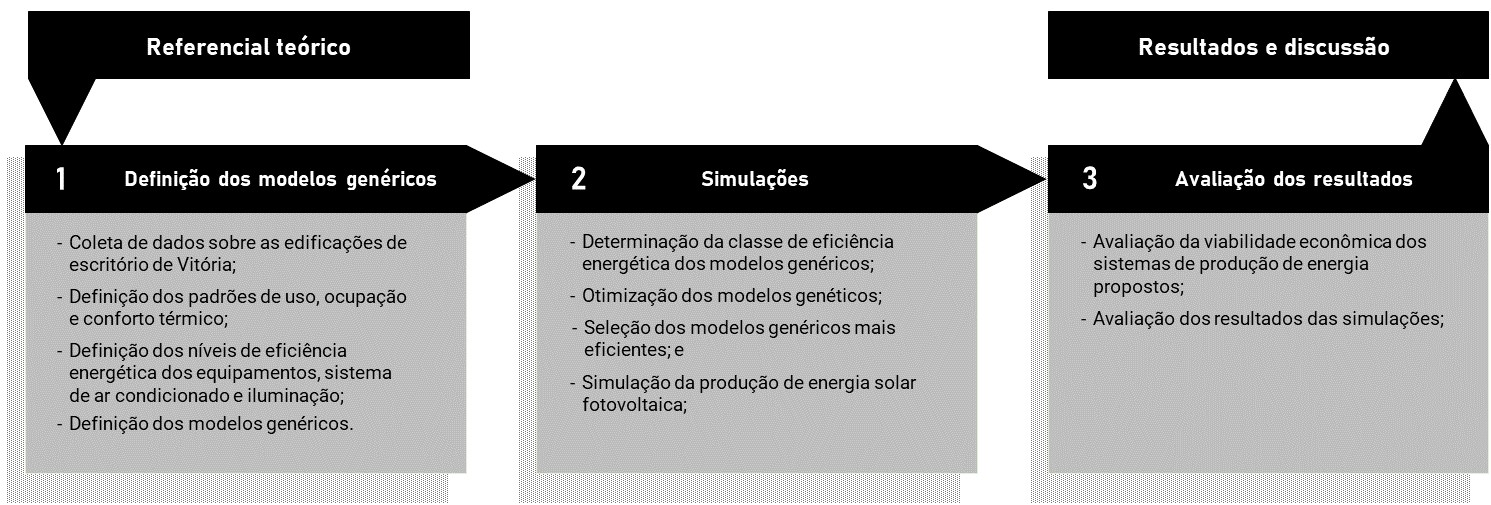
\includegraphics[width=1.0\textwidth]{figures/fig8_Fluxogramas_1.jpg}
    \begin{flushleft}
        \par \small Fonte: autor (2019).
    \end{flushleft}
    \label{fig:figura7}
\end{figure}%\vspace*{-0.3cm}
\subsection{Levantamento das características dos edifícios de escritório de Vitória}
As edificações de escritório de Vitória selecionadas após a definição do recorte 
territorial, apresentam características que foram complementadas aos atributos 
observados em edificações comerciais brasileiras, como suporte as informações não 
encontradas in loco. As características com maior frequência de ocorrência no 
levantamento realizado são apresentadas na Tabela \ref{tab:tabela4}. Todavia, a amostra coletada 
abrange edifícios iniciados em 2003 e concluídos até o fim do primeiro trimestre 
de 2018, data do início do levantamento. Este fato inviabiliza aplicar a última 
revisão do Plano à amostra.\vspace*{0.3cm} \newline
Foram considerados para o levantamento atributos como gabarito, número de 
pavimentos-tipo, número de salas por pavimento-tipo, dimensão e forma, altura 
dos pavimentos-tipo. Não foram consideradas as dimensões dos lotes onde as 
edificações da amostra estacam implantadas, já que este atributo não foi 
pertinente ao objetivo do trabalho. Estes parâmetros foram reunidos em consulta 
ao material técnico disponibilizado pelas construtoras, visitas a campo e 
complementação de dados utilizando a ferramenta computacional \textit{Google Street View}.\vspace*{0.3cm} \newline
Os trabalhos de \textcite{Lamberts2006,AmericanSocietyofHeatingRefrigeratingandAir-ConditioningEngineers-ASHRAE2010,Bernabe2012,Ramos2013,Didone2014,Didone2014a,ConselhoBrasileirodeConstrucaoSustentavel-CBCS2015,Fonseca2016,Werneck2017,InstitutoNacionaldeMetrologiaNormalizacaoeQualidadeIndustrial-INMETRO2018},
foram utilizados como principais fontes de informação para a análise de envoltória 
e sistema de iluminação e condicionamento de ar.\vspace*{-0.6cm}
\begin{table}[ht]\centering
    \caption{\small Características observadas em campo e em pesquisas anteriores.}
    \vspace*{0.2cm}
    \label{tab:tabela4}
    \begin{tabular*}{\columnwidth}{@{\extracolsep{\fill}}lll}
    \hline
    \textbf{Parâmetro}                                             & \textbf{Descrição}                                                                    & \textbf{Referências} \\ \hline
    Gabarito                                                       & 24 a 60 m (8 a 19 pav.)                                                               & \makecell[l]{Levantamento \textit{in loco} e referências\\ (BERNABÉ, 2012; CBCS, 2015; \\FONSECA et al., 2016; LAMBERTS; \\GHISI; RAMOS, 2006; RAMOS \\et al., 2013).} \\ \hline
    Altura do pavimento                                            & 3 m                                                                                   & Levantamento \textit{in loco}.                                                                                                                                         \\ \hline
    Planta-baixa (forma)                                           & Retangular                                                                            & \makecell[l]{Levantamento \textit{in loco} e referências\\ (FONSECA et al., 2016; INMETRO,\\ 2018).}                                                                   \\ \hline
    \makecell[l]{Dimensão das salas\\ por pav.-tipo}               & 40 m²                                                                                 & \makecell[l]{Foi fixado a área das salas \\(zonas térmicas) de acordo com a \\média de ofertas de salas observadas\\ em levantamento \textit{in loco}.}                  \\ \hline
    \multicolumn{3}{c}{Continua}\\\hline
    \end{tabular*}
\end{table}\pagebreak
\begin{table}[ht]\centering
    \begin{tabular*}{\columnwidth}{@{\extracolsep{\fill}}lll}
    \hline
    \multicolumn{3}{c}{Conclusão}\\\hline
    \makecell[l]{Componentes da\\ parede}                          & \makecell[l]{Bloco cerâmico,\\ 8 furos; \\14x19x29 cm; \\argamassa de\\ assentamento} & Levantamento \textit{in loco}.                                                                                                                                         \\ \hline
    Proteção solar                                                 & Sem proteção                                                                          & \makecell[l]{Levantamento \textit{in loco} e referências\\ (FONSECA et al., 2016; WERNECK \\et al., 2017).}                                                            \\ \hline
    Cobertura                                                      & \makecell[l]{Laje impermeabilizada\\ com 20 cm de\\ espessura}                        & \makecell[l]{Levantamento \textit{in loco} e referências \\(CB3E; ABIVIDRO, 2015).}                                                                                    \\ \hline
    Vidros                                                         & \makecell[l]{Laminado; Reflexivo;\\ 8 mm; Verde}                                      & \makecell[l]{(FONSECA et al., 2016; \\INMETRO, 2018).}                                                                                                                   \\ \hline
    PAF\textsubscript{T}                                           & 30\%; 50\%; 80\%                                                                      & \makecell[l]{Levantamento \textit{in loco}\\ e referências.}                                                                                                             \\ \hline
    \makecell[l]{Orientação solar da \\fachada principal}          & Sul                                                                                   & \makecell[l]{Levantamento \textit{in loco}\\ e referências.}                                                                                                             \\ \hline
    \makecell[l]{Densidade de Carga de\\ Iluminação Limite – DCIL} & 14,1 W/m²                                                                             & \makecell[l]{Consulta pública do RTQ-C \\(INMETRO, 2018).}                                                                                                               \\ \hline
    \makecell[l]{Densidade de Carga de\\ Equipamentos – DCE}       & 9,7 W/m²                                                                              & \makecell[l]{Consulta pública do RTQ-C \\(INMETRO, 2018).}                                                                                                               \\ \hline
    \makecell[l]{Absortância/transmitância \\das paredes}          & \makecell[l]{0,59 (cor \\camurça)/3,75}                                               & \makecell[l]{Valores consultados na \\NBR 15220-2 e referências \\(ABNT, 2003; FONSECA et \\al., 2016; INMETRO, 2018).}                                                                     \\ \hline
    \makecell[l]{Absortância/transmitância \\das coberturas}       & \makecell[l]{0,65 (concreto \\aparente)/2,06}                                         & \makecell[l]{Valores consultados na \\NBR 15220-2 e referências \\(ABNT, 2003; FONSECA et \\al., 2016; INMETRO, 2018).}                                                 \\ \hline
    \end{tabular*}
    \begin{flushleft}
        \par \small Fonte: autor (2019).
    \end{flushleft}
\end{table}\vspace*{-0.3cm}

\noindent As informações coletadas nos estudos e em levantamento formam a base conceitual para 
determinar os aspectos arquitetônicos relevantes para compor os modelos genéricos e, 
posteriormente, determinar os parâmetros de otimização e do consumo energético padrão 
aproximado para um edifício de escritório. Além disso, a quantidade de simulações necessárias 
para determinar o consumo de energia dos modelos genéricos é identificada por meio da 
organização dos dados coletados em campo e, assim, a resultante do número de variáveis.

\subsubsection{Consumo de energia elétrica das edificações}
\noindent O consumo de energia elétrica em edificações de escritório no Brasil é determinado 
principalmente por sua tipologia. As configurações predominantes no Brasil compreendem, em 
sua maioria, pequenas edificações, abaixo de 8 pavimentos, a edifícios grandes, acima de 
15 pavimentos \cite{Carlo2008,Ramos2013,ConselhoBrasileirodeConstrucaoSustentavel-CBCS2015,Fonseca2016}.\vspace*{0.3cm} \newline
\noindent Correlacionado às tipologias arquitetônicas, os dados de consumo de energia, expressos em 
Intensidade de Uso de Energia – IUE, kWh/m²/ano, foram necessários para validação das 
simulações iniciais quanto ao consumo de energia esperado dos modelos. Visto que a calibração 
dos modelos genéricos não foi possível, pois eles não dispunham de memorial de massa como 
ferramenta de comparação ao consumo simulado computacionalmente, foram adotados como método 
de comparação os valores médios registrados no Relatório Final do CBCS (2015), como mostra o 
Histograma no Gráfico 5. Foi relacionado o consumo de energia das edificações levantadas à 
frequência de ocorrência da quantidade de pavimentos de edificações comerciais brasileiras e 
suas respectivas áreas comuns.

    \begin{graph}
        \par \small Gráfico 5 - Consumo energético em edificações de escritório brasileiras.
        \begin{minipage}[ht]{1\textwidth}\centering
            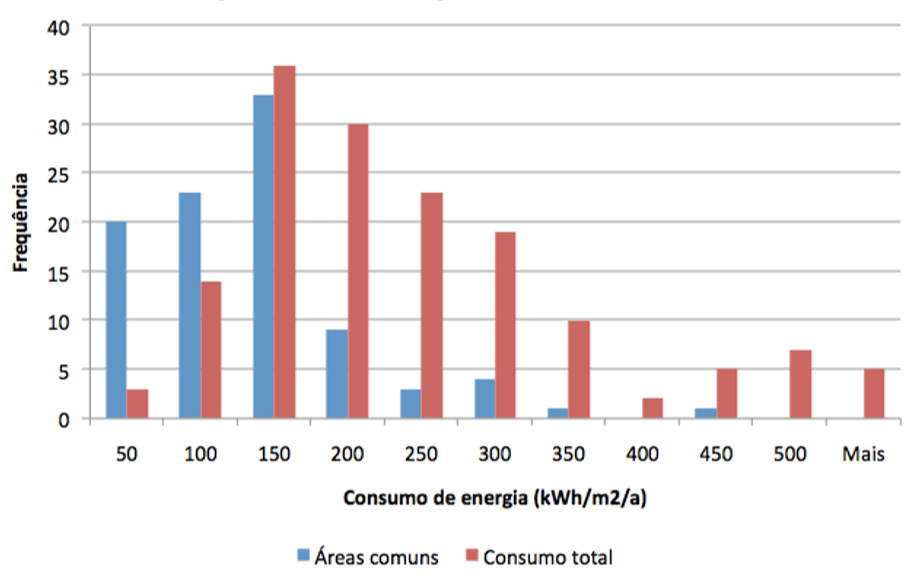
\includegraphics[width=0.85\textwidth]{figures/fig9_consumo-total-das-edificacoes-levantadas_cbcs_2015.png}            
        \end{minipage}
        \begin{flushleft}
            \par \small Fonte: adaptado de CBCS (2015).
        \end{flushleft}
    \end{graph}

\noindent Logo, os dados de IUE adotados para a comparação e avaliação inicial do consumo energético dos 
modelos foram baseados nos valores máximo e mínimo estabelecidos pelo CBCS (2015). A média 
entre o consumo em áreas comuns e total relacionado à frequência de quantidade de pavimentos 
define a quantidade total de consumo de energia para cada tipologia.\vspace*{0.3cm} \newline
Os autores do Relatório atribuem 133 kWh/m²/ano aos edifícios de pequeno porte, e 
268 kWh/m²/ano às edificações de grande porte. Vale ressaltar que os dados de consumo 
energético, assim como a média apontada no Relatório, de 191 kWh/m²/ano, desprezam as 
distorções causadas por edificações com particularidades de consumo como datacenters ou erros 
de cálculo de área útil.\vspace*{0.3cm} \newline
Ao estabelecer as Intensidades de Uso de Energia equivalentes a cada modelo, assim como os 
padrões de uso e ocupação, pode-se estimar o consumo de energia durante determinado período.

\subsubsection{Padrões de uso e ocupação em edifícios de escritório}
Os padrões de uso e ocupação da edificação foram baseados em normas, regulamentos, relatórios 
técnicos e referências acadêmicas que consideraram os níveis de atividades desenvolvidas nos 
ambientes, tratadas neste trabalho como zonas térmicas, como apresentado na Tabela \ref{tab:tabela5}.\vspace*{0.3cm} \newline
Como o intuito do trabalho foi criar modelos genéricos que representassem minimamente o 
cenário encontrado na cidade de Vitória, as características de uso e ocupação escolhidas 
foram integradas como forma de aproximar as tipologias ao cenário observado. Dentre elas, 
pode-se citar:
\begin{itemize}
    \item O nível metabólico apresentado em atividades de escritório;
    \item O horário de funcionamento dos escritórios, determinando os intervalos de tempo de ocupação total e parcial, onde, respectivamente, a capacidade máxima e parcial de ocupação das zonas térmicas é atingida;
    \item A densidade de pessoas por metro quadrado para cada zona térmica;
    \item A temperatura de conforto em cada zona térmica, de acordo com as normas de conforto térmico consultadas; e
    \item A umidade relativa do ar nos ambientes de escritório.
\end{itemize}

\noindent A obtenção dos dados acerca da atividade desempenhada nas edificações de escritório, além do 
horário de funcionamento e densidade de ocupação serão utilizados para estimar o consumo de 
energia elétrica do espaço utilizado por meio de simulação computacional.
\begin{table}[ht]\centering
    \caption{\small Padrões de uso e ocupação}
    \vspace*{0.2cm}
    \label{tab:tabela5}
    \begin{tabular*}{\columnwidth}{@{\extracolsep{\fill}}llll}
        \hline
        \textbf{Parâmetro}                                & \multicolumn{2}{c}{\textbf{Descrição}}                                                                                             & \textbf{Referências} \\ \hline
        \multirow{2}{*}{Atividades}                       & \makecell[l]{Escritório:\vspace*{0,2cm}\\Fator metabólico:\vspace*{0,2cm}} & \makecell[l]{Leve\vspace*{0,2cm}\\0,9 met}                  & \makecell[l]{As salas de escritório da cidade\\
                                                                                                                                                                                        são utilizadas, em sua maioria,\\ para 
                                                                                                                                                                                        atividades especializadas de\\ âmbito 
                                                                                                                                                                                        jurídico, relacionadas à \\construção 
                                                                                                                                                                                        civil, a saúde e atividades\\ financeiras.} \\ \hline
        \multicolumn{4}{c}{Continua}\\\hline
    \end{tabular*}
\end{table}\pagebreak
\begin{table}[ht]\centering
        \begin{tabular*}{\columnwidth}{@{\extracolsep{\fill}}llll}
        \hline
        \multicolumn{4}{c}{Conclusão}\\\hline
        \multirow{2}{*}{Horário de funcionamento}                          & \makecell[l]{Ocupação\\ total:\vspace*{0,2cm}\\Ocupação \\parcial (50\%):\vspace*{0,6cm}}  & \makecell[l]{8h às 12h; \\13h às 18h \vspace*{0,6cm}\\12h às 13h} & \makecell[l]{Segundo normas e pes-\\quisas
                                                                                                                                                                                                                                                sobre o horário de\\ funcionamento de 
                                                                                                                                                                                                                                                escri-\\tórios, o início da ocupa-\\ção se 
                                                                                                                                                                                                                                                dá às 6h e pode se\\ estender até às 24h.\\ 
                                                                                                                                                                                                                                                Entretanto, visando a\\ aproximação às 
                                                                                                                                                                                                                                                condi-\\ções praticadas no\\ mercado brasileiro,\\ 
                                                                                                                                                                                                                                                adota-se a redução\\ de ocupação durante\\ o 
                                                                                                                                                                                                                                                horário de almoço, \\denominada ocupação\\ parcial.}  \\ \hline
        Densidade de ocupação                             & \multicolumn{2}{c}{0,14 pessoas/m²} & \makecell[l]{(CONSELHO BRASILEIRO\\ DE CONSTRUÇÃO 
                                                                                                  SUS-\\TENTÁVEL - CBCS, 2015;\\ LAMBERTS; 
                                                                                                  GHISI;\\ RAMOS, 2006; MORAES;\\ PEREIRA, 2014).} \\ \hline
        Temperatura de controle                           & \multicolumn{2}{c}{24°C}            & \makecell[l]{Temperatura limite de\\ acionamento
                                                                                                  do sistema de\\ condicionamento de\\ ar (ASHRAE, 
                                                                                                  2010, 2017a;\\ INMETRO, 2010a).} \\ \hline
        \makecell[l]{Nível de iluminância\\ de referência}& \multicolumn{2}{c}{500 lux}         & \makecell[l]{Iluminância mínima (entor-\\no de 
                                                                                                  trabalho) para ativi-\\dades visuais 
                                                                                                  (ASHRAE,\\ 2010; ABNT, 2013).} \\ \hline
        \makecell[l]{Umidade Relativa\\ Interna}          & \multicolumn{2}{c}{40\%-60\%}       & \makecell[l]{Faixa recomentada pela\\
                                                                                                  ASHRAE 55 (2017a).}\\ \hline
    \end{tabular*}
    \begin{flushleft}
        \par \small Fonte: autor (2019).
    \end{flushleft}
\end{table}\vspace*{-0.5cm}
\subsection{Padrões de conforto}
O conforto térmico e de iluminação natural são parâmetros essenciais para a avaliação 
da qualidade do ambiente em que se vive. Não obstante, é necessário estabelecer padrões 
de conforto para a simulação de desempenho termoenergético do modelo genérico. Os 
próximos subitens tratam dos parâmetros adotados para a posterior inserção de dados 
e informações nos processos de simulação.
\subsubsection{Conforto térmico}
Utilizando os conceitos de conforto adaptativo, foi calculada a temperatura de conforto (t\textsubscript{c}) 
descrita pela \textcite{AmericanSocietyofHeatingRefrigeratingandAir-ConditioningEngineers-ASHRAE2017}, e assim estipulada a faixa de temperaturas de conforto e 
set point para controle de temperatura dos ambientes dos modelos genéricos. Este modelo 
avalia a adaptação do usuário em diferentes campos como o fisiológico, o comportamental 
e o psicológico \cite{AmericanSocietyofHeatingRefrigeratingandAir-ConditioningEngineers-ASHRAE2017a} e pode ser expresso pela Equação \ref{eq:eq1} tratada no Referencial Teórico.\vspace*{0.3cm} \newline
Foram utilizadas as temperaturas de bulbo seco máximas e mínimas como valores representantes 
da temperatura externa da edificação \cite{InstitutoNacionaldeMetereologia-INMET2018}. Estes dados de temperatura serão 
fundamentais para a caracterização do meio em que o modelo genérico será simulado, 
influenciando no desempenho simulado da envoltória e dos sistemas de condicionamento de ar 
e iluminação.
\subsubsection{Conforto lumínico}
A norma NBR/ISO CIE 8995-1 \cite{AssociacaoBrasileiradeNormasTecnicas-ABNT2013} determina que a condição de conforto visual 
em ambientes de escritório requer valor igual ou maior que 500 lux de iluminância de entorno 
imediato da tarefa a ser desempenhada \cite{AssociacaoBrasileiradeNormasTecnicas-ABNT2013,Ramos2013}. Assegurar a 
iluminância é uma condição importante para garantir o conforto, desempenho e segurança visual 
aos usuários, seja por fonte luminosa artificial ou natural.\vspace*{0.3cm} \newline
Para que a iluminação interna se mantenha dentro do padrão estabelecido por norma, foi 
necessário calcular o Fator de Luz Diurna – FDL, como forma de verificar se a adoção 
iluminância proposta pela norma seria adequada as condições empregadas aos modelos de 
referência. Este fator, uma vez incorporado nas rotinas de simulação computacional, 
influencia diretamente nas condições de iluminação no ambiente, indicando se estão adequadas 
para a realização de tarefas que exigem um determinado volume de iluminação.\vspace*{0.3cm} \newline
Considerando a ocupação anual parcial dos ambientes, foi possível estabelecer a relação 
entre a iluminância interna desejada, 500 lux, e a mediana da iluminância difusa horizontal 
externa, dado retirado do arquivo climático de Vitória \cite{InstitutoNacionaldeMetrologiaNormalizacaoeQualidadeIndustrial-INMETRO2018}, de 50019,16 lux. 
Assim, o FLD necessário para manter a iluminância interna das salas de escritório durante o 
período de ocupação levantado pode ser expresso pela Equação \ref{eq:eq2}.
\begin{equation}\label{eq:eq2}
    FLD=\frac{E_{interna}}{E_{externa}}*100
\end{equation}

Onde:\par
\setlength\parindent{1.5cm} \textit{FLD} é o Fluxo de Luz Diurna, em porcentagem;\par
\setlength\parindent{1.5cm} E\textsubscript{interna} é a iluminância interior em um ponto de um plano, em lux; e\par
\setlength\parindent{1.5cm} E\textsubscript{externa} é a iluminância externa simultânea em um plano horizontal, em lux.\vspace*{0.3cm} \newline
\noindent Concluída a caracterização dos padrões de conforto a serem avaliados, são definidos os 
parâmetros para os níveis de eficiência energética esperados dos equipamentos de 
condicionamento de ar e iluminação artificial presentes no modelo genérico. A partir desta 
definição embasada em regulamentos como o INI-C, é possível estimar a otimização de consumo 
energético da edificação proposta.
\subsection{Níveis de eficiência energética}
Os níveis de eficiência dos aparelhos utilizados na manutenção do conforto da edificação 
exercem importante papel quando há a necessidade de racionamento do consumo energético. 
Para tal, estes aparelhos são avaliados segundo critérios de desempenho energético e, ao 
final dessa avaliação, é atribuído um índice representativo da eficiência energética 
alcançada. Os índices de desempenho apresentados neste trabalho foram baseados na 
Instrução Normativa Inmetro para Classe de Eficiência Energética de Edificações Comerciais, 
de Serviços e Públicas – INI-C.
\subsubsection{Determinação da classe de eficiência energética dos modelos genéricos}
As primeiras simulações energéticas servem como meio de ajuste e verificação de erros 
entre os dados de saída de consumo energético e intensidade de uso de energia. Os 
resultados das simulações iniciais foram comparados às análises feitas de Determinação 
de Classe de Desempenho Energético, baseado na metodologia do INI-C, e nos resultados 
apresentados pelo Relatório Final de Desempenho Energético do CBCS. A partir da 
discrepância dos valores obtidos entre as simulações iniciais e as referências 
selecionadas, foram realizados ajustes a fim de adequar o modelo computacional à 
tolerância estabelecida.\vspace*{0.3cm} \newline
Os modelos genéricos foram avaliados segundo a definição da Instrução Normativa, onde 
é definido que o Modelo Real representa a edificação a ser classificada, enquanto 
o Modelo de Referencia representa a edificação com baixo desempenho energético. 
Desta forma, os edifícios propostos são comparados com um modelo de baixa performance, 
evidenciando, assim, seu desempenho energético. As variáveis analisadas para a 
comparação com o Modelo de Referência foram o consumo de energia térmica, elétrica 
e primaria dos modelos.\vspace*{0.3cm} \newline
A partir do diagnóstico de desempenho energética dos modelos genéricos, foram 
implementadas as otimizações e medidas de produção de energia em contraponto ao 
consumo energético constatado em simulação.
\subsubsection{Eficiência energética do sistema de condicionamento de ar}
Os sistemas de condicionamento de ar presentes em edifícios de escritório são 
compostos basicamente por dois tipos de equipamentos: ar-condicionado Split e o 
Sistema Central de Água Gelada – CAG \cite{ConselhoBrasileirodeConstrucaoSustentavel-CBCS2015}.\vspace*{0.3cm} \newline
Segundo o \textcite{InstitutoNacionaldeMetrologiaNormalizacaoeQualidadeIndustrial-INMETRO2018}, esses equipamentos são classificados segundo a 
capacidade de resfriamento e a potência absorvida pelos motores em pleno 
funcionamento. Esta relação é representada pelo Coeficiente de Performance – COP, 
expresso em W/W. O COP para equipamentos de ar condicionado é categorizado 
segundo uma Classe de Eficiência Energética – CEE, como apresentado na Tabela \ref{tab:tabela6}.

\begin{table}[ht]\centering
    \caption{\small  Relação entre o COP e as Classes de Eficiência Energética de Condicionadores de ar.}
    \vspace*{0.3cm}
    \label{tab:tabela6}
    \begin{tabular}{cccc}
        \hline
        \textbf{Classes}     & \multicolumn{3}{c}{\textbf{Densidade de Potência de Iluminação (DPI – W/m²)}}        \\ \hline
        A                    & \makecell[c]{3,23}       & \makecell[c]{\textless CEE}                  &            \\ \hline
        B                    & \makecell[c]{3,02}       & \makecell[c]{\textless CEE =\textless} & 3,23       \\ \hline
        C                    & \makecell[c]{2,81}       & \makecell[c]{\textless CEE =\textless} & 3,02       \\ \hline
        D                    & \makecell[c]{2,60}       & \makecell[c]{\textless CEE =\textless} & 2,81       \\ \hline
    \end{tabular}
    \begin{flushleft}
        \par \small Fonte: adaptado de INMETRO (2018).
    \end{flushleft}
\end{table}\vspace*{-0.5cm}

\noindent Esta classificação atribuída ao sistema de ar condicionado dos modelos genéricos, juntamente 
ao nível de eficiência energética do sistema de iluminação, é essencial para a etapa de 
simulação e identificação do consumo final de energia dos modelos genéricos, representantes 
do cenário observado dentro do recorte territorial.\vspace*{0.3cm} \newline
Como o sistema mais frequente observado nas edificações levantadas foi o Sistema Central 
de Água Gelada – CAG, com volume de ar constante, e este, tomando como base os modelos mais 
populares do mercado brasileiro, possui COP base próximo a classe “D” por demandar muita 
energia à sua operação, foi utilizado o valor de COP indicado à classe “D” pela tabela da 
INI-C. Posterior a etapa de determinação de classe, foi feita a substituição dos aparelhos 
pertencentes à classe “D” – 2,60, para a classe “A” – 3,23 como forma de otimização 
utilizando estratégia ativa de redução de consumo de energia.
\subsubsection{Eficiência energética do sistema iluminação artificial e equipamentos}
A eficiência do sistema de iluminação e equipamentos de um edifício de escritório, tal 
qual o sistema de condicionamento de ar, representa uma parcela importante no consumo 
final de energia elétrica da edificação \cite{AmericanSocietyofHeatingRefrigeratingandAir-ConditioningEngineers-ASHRAE2019,ConselhoBrasileirodeConstrucaoSustentavel-CBCS2015}.\vspace*{0.3cm} \newline
Dessa forma, para certificar que o sistema de iluminação artificial seja energeticamente 
eficiente e reduza o impacto desse sistema no consumo de energia elétrica, é avaliada a 
razão entre o somatório das potências das lâmpadas e reatores instalados e a área de um 
ambiente ou zona térmica, razão denominada como Densidade de Potência de Iluminação – DPI, 
expressa em W/m². O mesmo procedimento é aplicado aos equipamentos, definidos pela Densidade 
de Potência de Equipamentos – DPE, expressa em W/m². A união das duas densidades é definida 
pela Densidade de Carga Interna – DCI.\vspace*{0.3cm} \newline
Após a avaliação do DPI, os equipamentos de iluminação artificial são classificados 
segundo a classe de eficiência energética estabelecida pelo PBE/Inmetro, conforme a Tabela \ref{tab:tabela7}.

\begin{table}[ht]\centering
    \caption{\small Densidades de Potência de Iluminação definidas pelo INI-C e as Classes de Eficiência Energética.}
    \vspace*{0.3cm}
    \label{tab:tabela7}
    \begin{tabular}{cc}
        \hline
        \textbf{Classes}                & \textbf{Densidade de Potência de Iluminação (DPI – W/m²)}\\ \hline
        A                               & 8,50                                                     \\ \hline
        B                               & 10,40                                                    \\ \hline
        C                               & 12,20                                                    \\ \hline
        D                               & 14,10                                                    \\ \hline
    \end{tabular}
    \begin{flushleft}
        \par \small Fonte: adaptado de INMETRO (2018).
    \end{flushleft}
\end{table}\vspace*{-0.5cm}
\noindent Assim como o sistema de condicionamento de ar, a definição da DPI possibilita classificar o 
sistema de iluminação artificial do modelo genérico segundo sua eficiência energética. 
Para a determinação da classe de eficiência energética, o procedimento é o mesmo adotado 
para definição do COP para a etapa de simulação, e neste caso, como os equipamentos 
elétricos e de iluminação não foram levantados nominalmente, partiu-se da situação requerida 
e indicada pelo INI-C, com DPI classe “D”, de 14,10 W/m², e equipamentos com DPE de 9,7 W/m². 
Desta forma, espera-se que seja evidenciada a influência do sistema de iluminação no 
contexto geral de otimização da edificação.


\subsection{Definição dos modelos genéricos}
Com base no INI-C (2018) e no levantamento das edificações de escritório de Vitória, foram propostos dois tipos de modelos genéricos como base para o estudo das modificações de otimização e de produção de energia. Estes modelos representam os dois cenários de ambiente construído mais observados na cidade de Vitória. Estes cenários são formados por edificações mais baixas, com 8 pavimentos, e as mais altas, com 19 pavimentos. As dimensões utilizadas como referência para a construção dos modelos genéricos foram resultado dos valores médios observados nas edificações que compõe o levantamento.\vspace*{0.3cm} \newline
As características predominantes aplicadas aos modelos genéricos foram:
    \begin{itemize}\vspace*{-0.3cm}
        \item Número de pavimentos;\vspace*{-0.3cm}
        \item Forma - retangular;\vspace*{-0.3cm}
        \item Altura - gabarito e dimensões das fachadas;\vspace*{-0.3cm}
        \item Layout interno dos pavimento-tipo;\vspace*{-0.3cm}
        \item Ausência de proteção solar;\vspace*{-0.3cm}
        \item Percentual Total de Área de Abertura da Fachada.\vspace*{-0.3cm}
    \end{itemize}
A composição dos modelos é baseada nas características predominantes e nos dados coletados \textit{in site}.\vspace*{-0.5cm} \newline
\subsubsection{Composição dos modelos genéricos}
A composição construtiva atribuída aos modelos utilizados neste trabalho mostra fundamentalmente 
os parâmetros necessários para a avaliação do desempenho energético segundo o INI-C. Os atributos utilizados serviram como ponto de partida para as análises subsequentes sugeridas nas 
etapas metodológicas e estão dispostos no Fluxograma da Figura \ref{fig:figura8}.\vspace*{0.5cm}\pagebreak
    %\vspace*{-1cm}
    \begin{figure}[H]
        \centering
        \caption{\small Fatores utilizados como parâmetros de configuração volumétrica dos modelos genéricos.}
        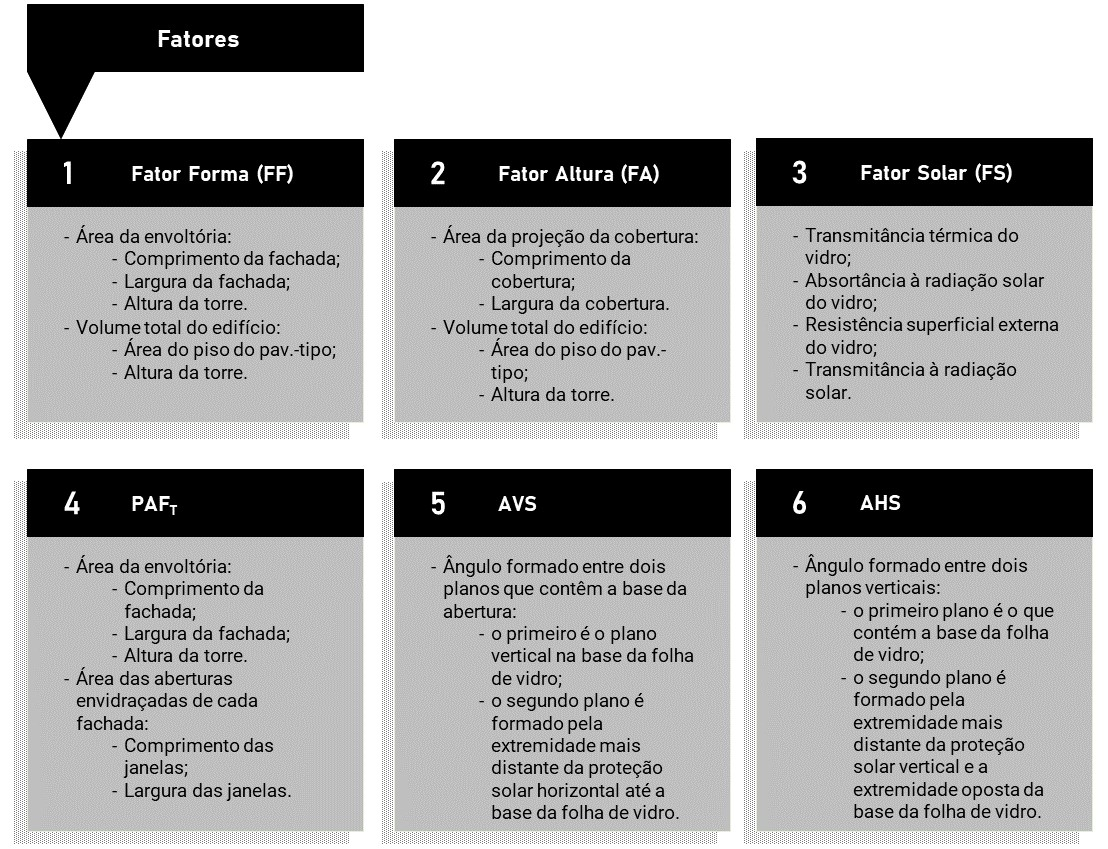
\includegraphics[width=0.8\textwidth]{figures/fig10_Fluxogramas-2.jpg}
        \begin{flushleft}
            \par \small Fonte: autor (2019)
        \end{flushleft}
        \label{fig:figura8}
    \end{figure}\vspace*{-0.6cm}

\noindent Apresentados na Tabela 7 e exemplificado na Figura \ref{fig:figura9}, os atributos estudados foram Fator de Forma, FF, Fator Altura, FA, Percentual de Área de Abertura da Fachada Total, PAFT, Ângulo Vertical de Sombreamento, AVS, e Ângulo Horizontal de Sombreamento, AHS.\vspace*{0.3cm}
\begin{figure}[H]
    \centering
    \caption{\small Estrutura arquitetônica dos modelos genéricos.}
    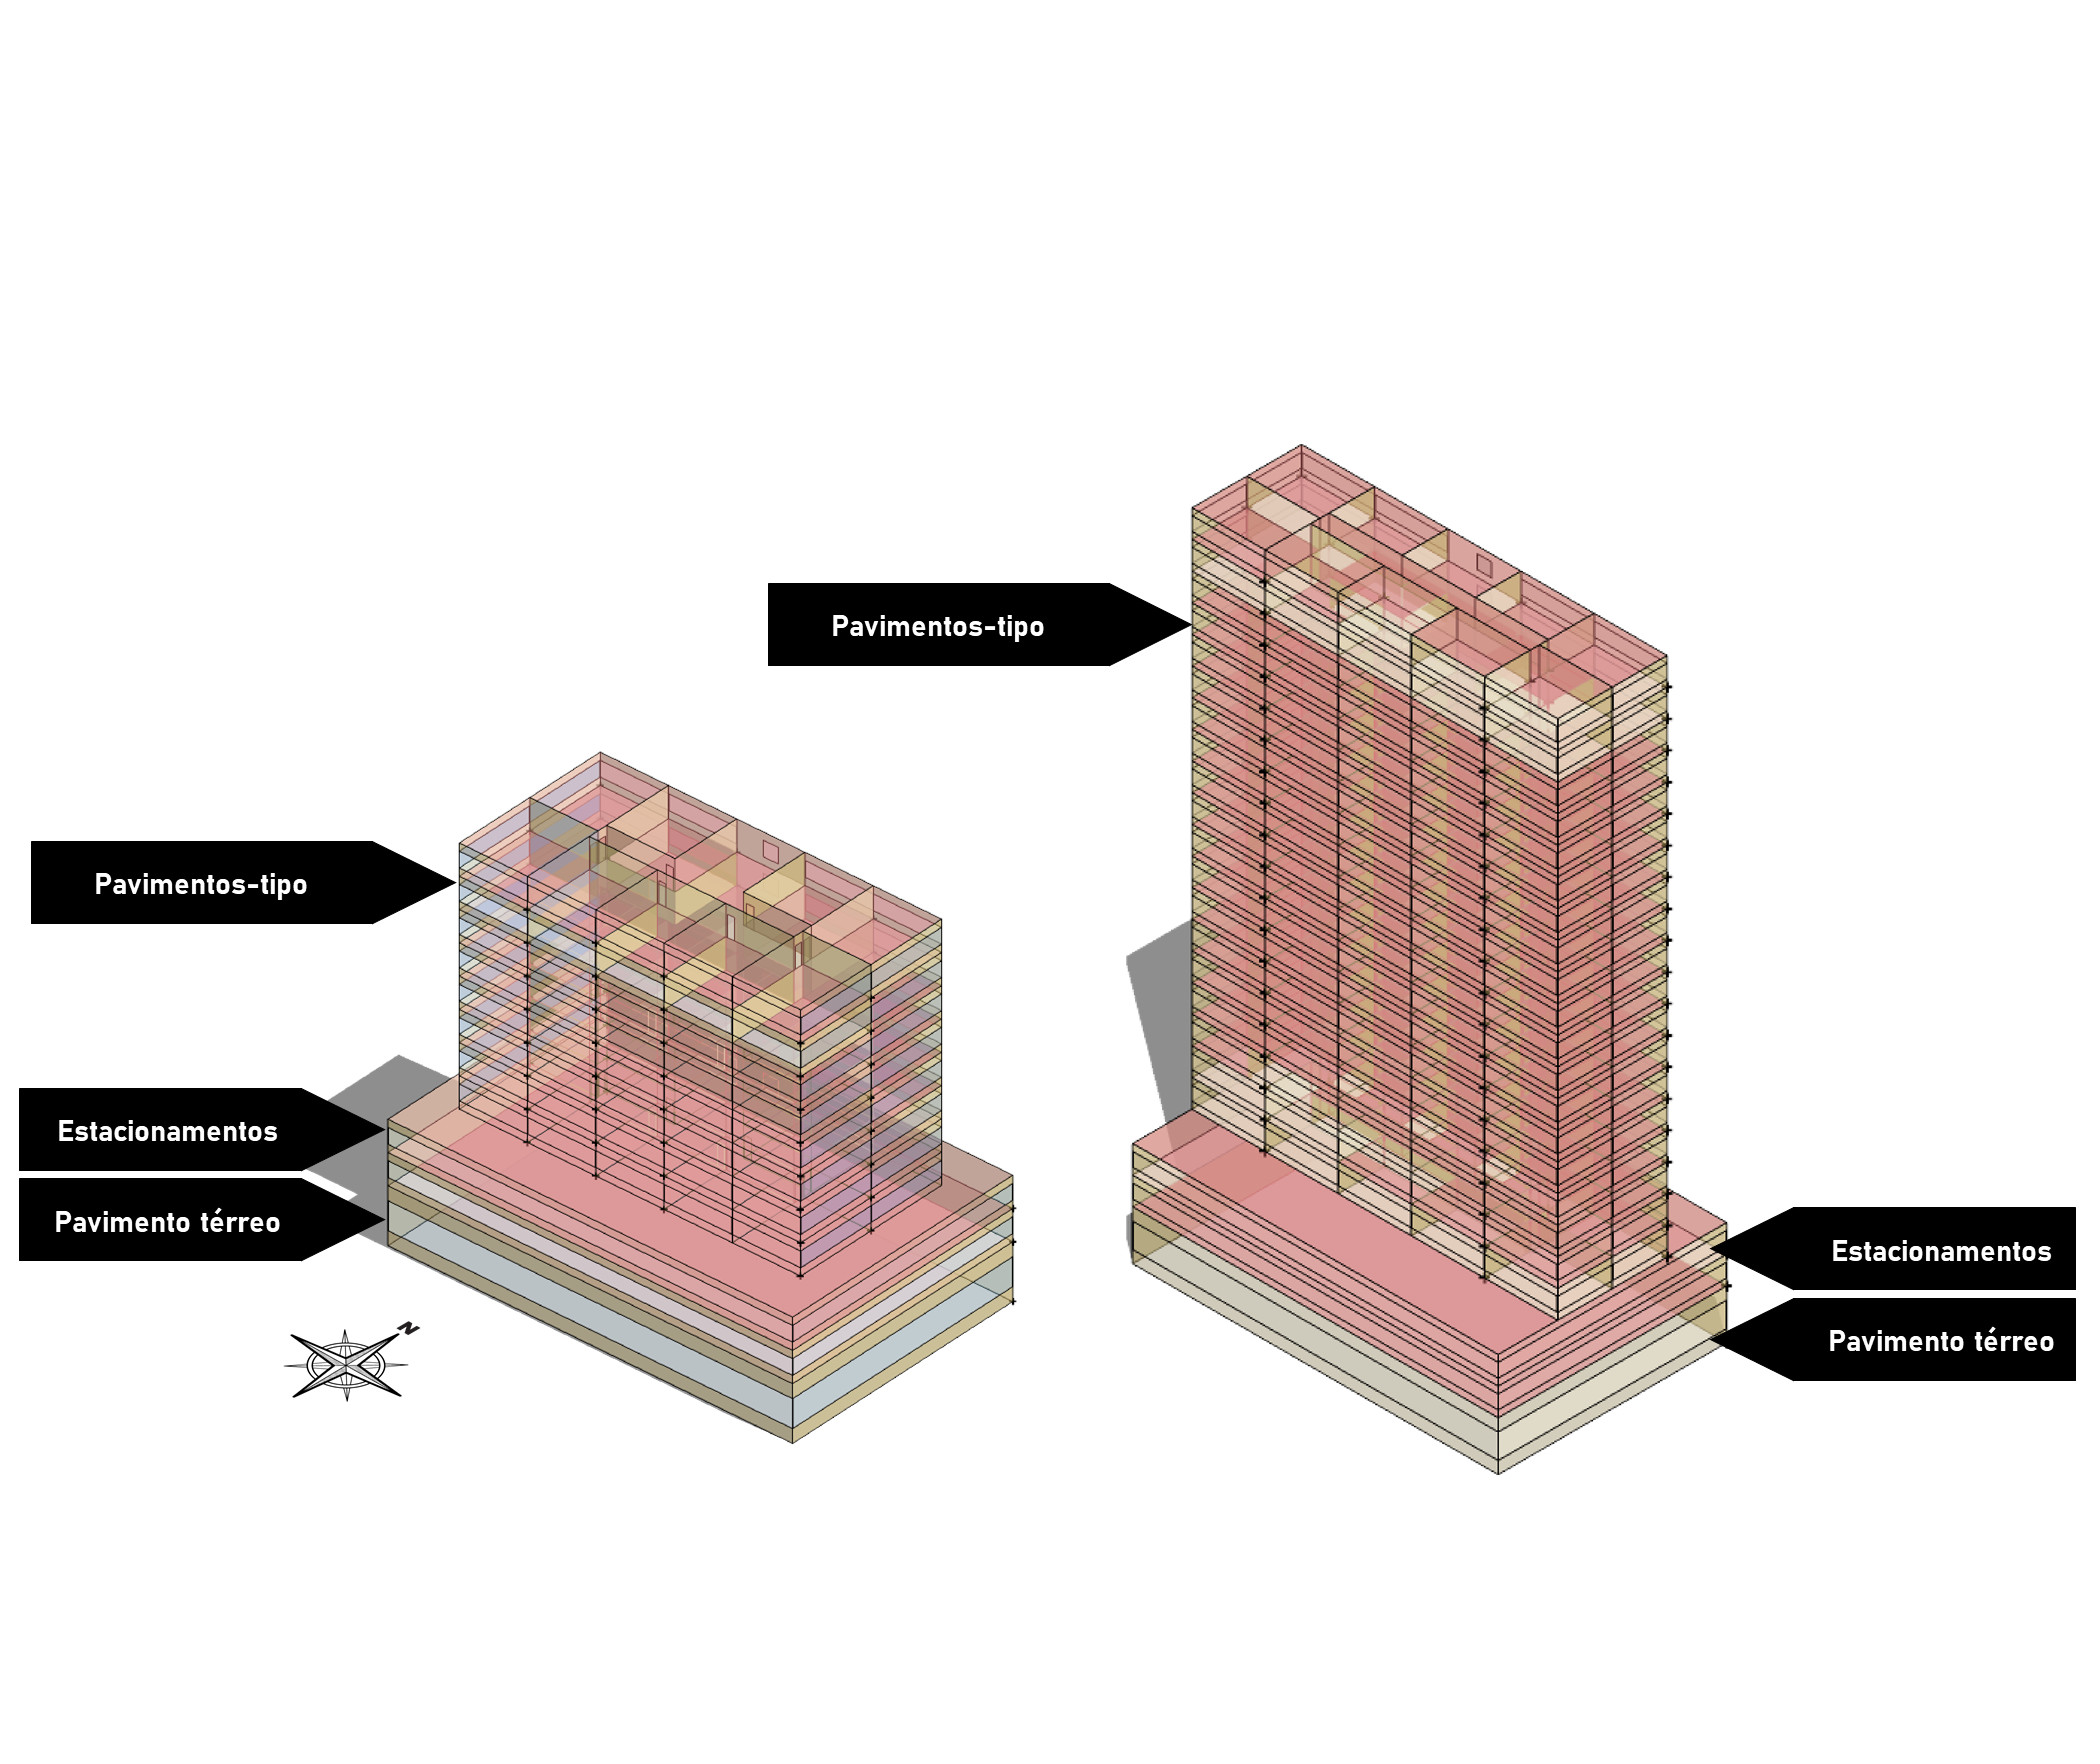
\includegraphics[width=0.9\textwidth]{figures/fig11_8-19-2pav.png}
    \begin{flushleft}
        \par \small Fonte: autor (2019).
    \end{flushleft}
    \label{fig:figura9}
\end{figure}

\noindent O PAF\textsubscript{T} e as propriedades do vidro utilizados para os modelos genéricos, como Fator Solar – FS, ou Solar Heat Gain Coefficient – SHGC, foram adotados considerando as médias desses atributos coletados in loco e complementados por dados extraídos do Catálogo de Propriedades Térmicas e Óticas de Vidro \cite{CentroBrasileirodeEficienciaEnergeticaemEdificacoesCB3E2015,AssociacaoBrasileiradeNormasTecnicas-ABNT2003}, da NBR 15220 (2003) e do INI-C \cite{InstitutoNacionaldeMetrologiaNormalizacaoeQualidadeIndustrial-INMETRO2018}, 
como forma de tornar genéricos os dados empregados, como apresentado na Tabela \ref{tab:tabela8}.%\vspace*{0.3cm} \newline
\begin{table}[H]\centering
    \caption{\small Parâmetros arquitetônicos dos modelos genéricos.}
    \vspace*{0.3cm}
    \label{tab:tabela8}
    \begin{tabular*}{\columnwidth}{@{\extracolsep{\fill}}l|ll}
    \hline
    \textbf{Parâmetro}                                                              & \textbf{Descrição}         & \textbf{Referências}  \\ \hline
    \multicolumn{3}{c}{\textbf{Dados dimensionais dos pavimentos-tipo}}\\\hline
    Número de pavimento (un)                                                        & 8                          & 19                    \\ \hline
    \makecell[l]{Proporção geométrica – pav.\\ tipo (m – Comprimento x Largura)}    & 33,75x16                   & 40x12                 \\ \hline
    Altura do pavimento-tipo (m)                                                    & 3                          & 3                     \\ \hline
    \makecell[l]{Área total construída – pavimentos-tipo (m²)}                      & 4.320                      & 9.120                 \\ \hline
    Área de projeção da cobertura - Apcob (m²)                                      & 843,75                     & 640,00                \\ \hline
    Área de projeção do edifício - Ape (m²)*                                        & 1000                       & 1000                  \\ \hline
    Área total construída - Atot (m²)                                               & 7.320                      & 12.120                \\ \hline
    Volume Total da Edificação - Vtot (m³)                                          & 24.360                     & 38.760                \\ \hline
    Área da envoltória - Aenv (m²)                                                  & 5.430,30                   & 8.890,00              \\ \hline
    Fator de Forma (FF)                                                             & 0,222                      & 0,229                 \\ \hline
    Fator Altura (FA)                                                               & 0,125                      & 0,052                 \\ \hline
    Fator Solar (FS)                                                                & 0,44                       & 0,44                  \\ \hline
    Transmitância do vidro (W/m²K)                                                  & 5,6                        & 5,6                   \\ \hline
    Área de aberturas das fachadas – Aabert (m²)                                    & 1.501,80                   & 3.152,40              \\ \hline
    PAF\textsubscript{T} (\%)                                                       & 50\%                       & 50\%                  \\ \hline
    \makecell[l]{Ângulo Vertical (AVS) e Horizontal\\ (AHS) de Sombreamento (°)}    & 0                          & 0                     \\ \hline
    \end{tabular*}
    \begin{flushleft}
        \par \small Fonte: autor (2019); *A Ape contempla a área de projeção do pavimento térreo e estacionamentos.
    \end{flushleft}
\end{table}

\noindent Segundo o INI-C, publicado pelo \textcite{InstitutoNacionaldeMetrologiaNormalizacaoeQualidadeIndustrial-INMETRO2018},
a utilização do Ângulo de Obstrução Vertical – AOV, para a simulação de obstruções solares parciais e totais são critérios opcionais que dependem da condição real levantada. Apesar da obstrução solar lateral ter sido uma condição observada em algumas edificações de Vitória, com base na observação da frequência de ocorrência, este atributo não foi considerado para o presente trabalho dada a configuração e disposição das edificações do recorte territorial em relação ao lote, que possibilitaram utilizar cenários sem obstrução solar. Além disso, para o estudo da incidência de radiação solar sobre a edificação e como ponto de partida para a implementação das estratégias passivas aos modelos genéricos, foi definido a fachada principal com orientação Sul, de acordo com a frequência de ocorrência observada na amostragem.\vspace*{0.3cm} \newline
O pavimento térreo e dois pavimentos de estacionamentos (Figura \ref{fig:figura10}), foram centralizados na base das torres em ambos os modelos, com dimensões idênticas e de forma genérica, com o intuito de evidenciar a influência sobre o consumo energético total por meio do número de pavimentos. Contudo, o uso e ocupação destas áreas se torna de baixa relevância, uma vez que as atividades de maior permanência se dão nos ambientes da torre.\vspace*{0.3cm} \newline
Estes pavimentos compreendem características arquitetônicas apresentadas em todas as edificações selecionadas em levantamento. Posteriormente, na etapa de produção de energia, foi proposto o deslocamento dos pavimentos abaixo da torre para aproveitamento de área para inserção de painéis fotovoltaicos.
\begin{figure}[H]
    \centering
    \caption{\small Conformação do pavimento térreo e estacionamentos.}
    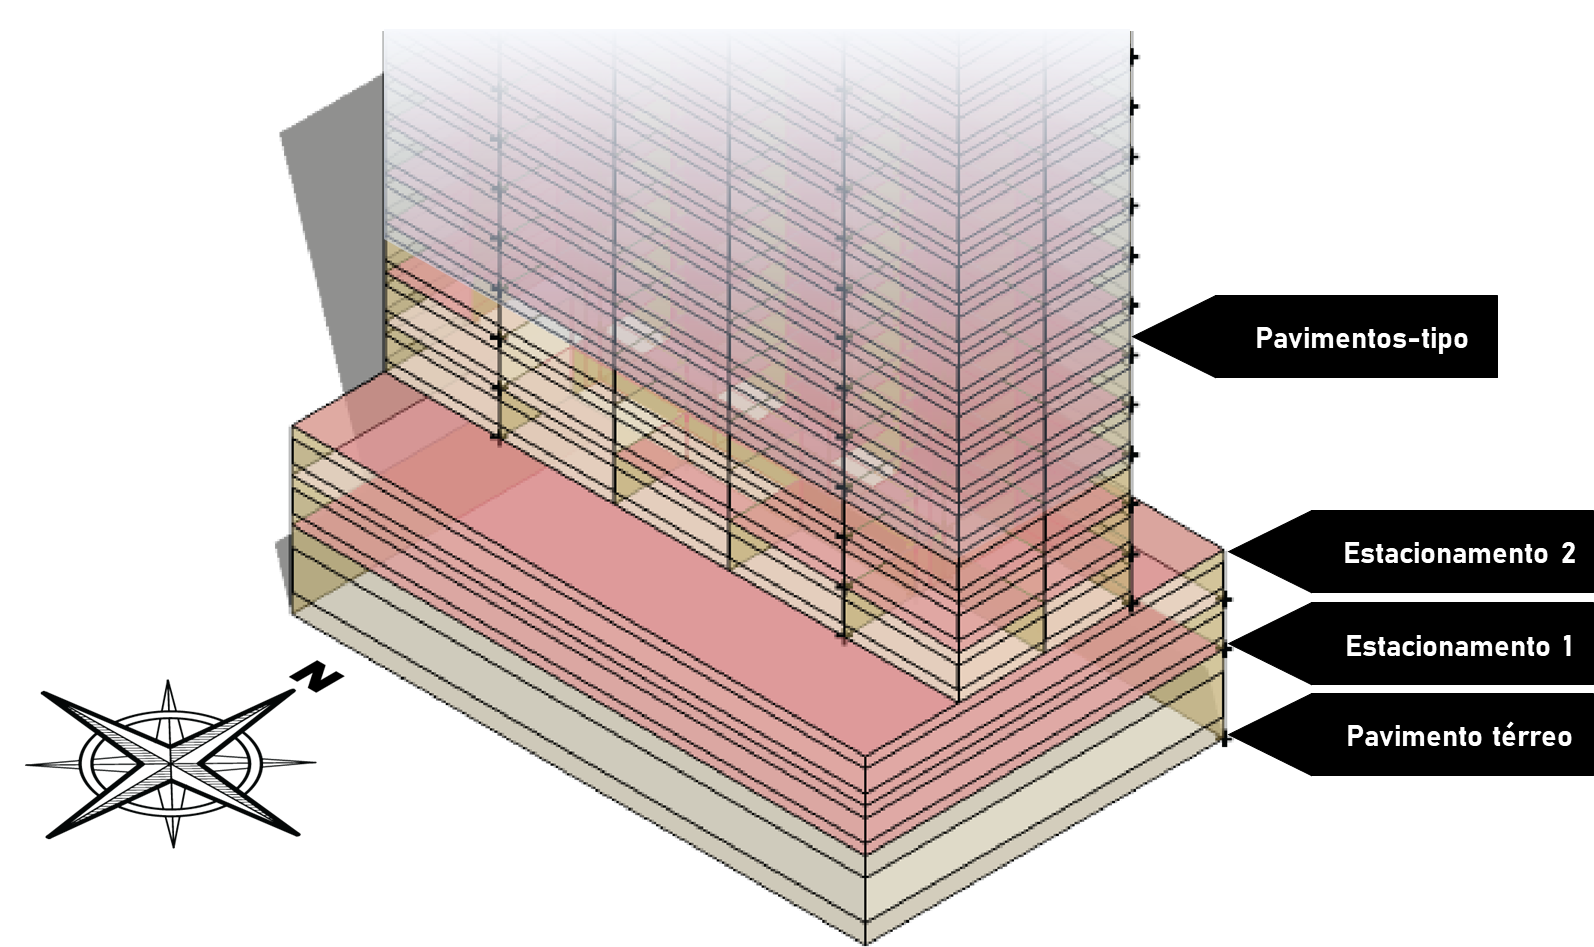
\includegraphics[width=0.9\textwidth]{figures/fig12-base_torre-1.png}
    \begin{flushleft}
        \par \small Fonte: autor (2019).
    \end{flushleft}
    \label{fig:figura10}
\end{figure}\vspace*{-0.5cm}
\noindent Os modelos são distinguidos principalmente pela área de projeção, número de pavimentos, pelo volume total e área da envoltória. Esses fatores resultam diretamente em Fator de Forma e Fator Altura distintos para cada modelo, amparando um dos objetivos específicos desta pesquisa sobre identificar as características mais influentes no consumo de energia elétrica. As zonas térmicas também formam características distintas entre os modelos genéricos, variando as áreas úteis, como apresentado na Tabela \ref{tab:tabela9}.
\begin{table}[H]
    \centering
    \caption{\small Zonas térmicas dos modelos genéricos.}
    \begin{tabular*}{\columnwidth}{@{\extracolsep{\fill}}ll}\hline
        \makecell[c]{Zonas térmicas - modelo\\ genérico de 8 pavimentos}                    & \makecell[c]{Zonas térmicas - modelo \\genérico de 19 pavimentos}                 \\ \hline
        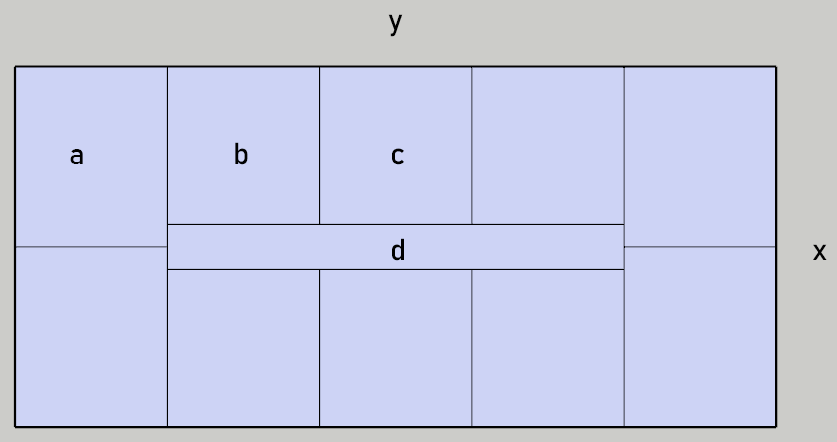
\includegraphics[width=0.5\textwidth]{figures/tab9-pb-8pav.png}                     & 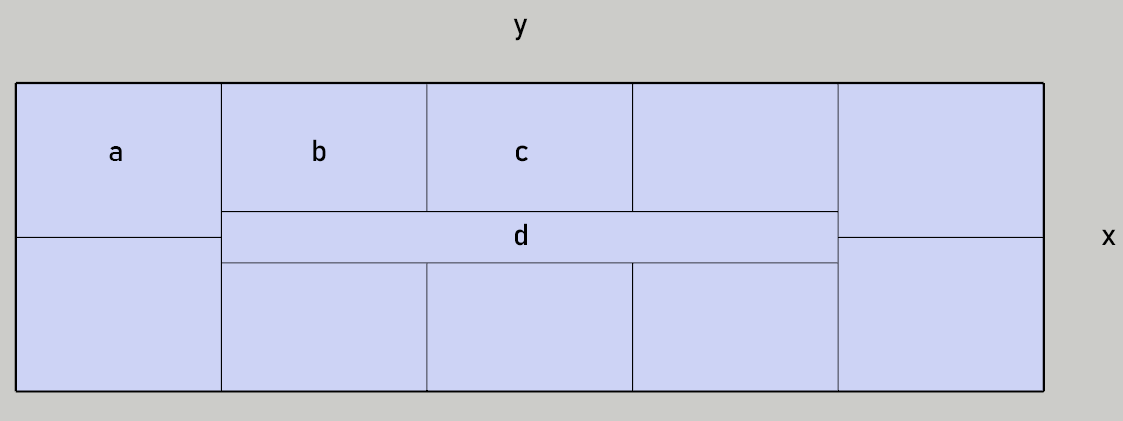
\includegraphics[width=0.5\textwidth]{figures/tab9-pb-19pav.png}                  \\
        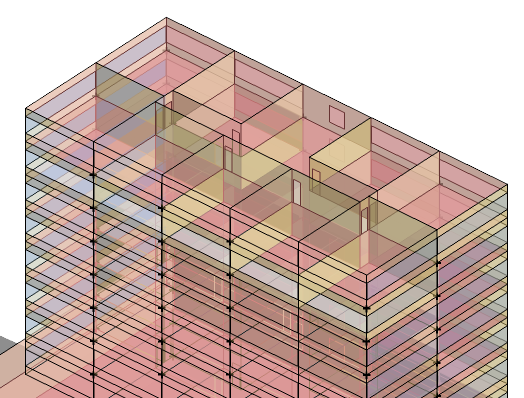
\includegraphics[width=0.5\textwidth]{figures/tab9-CEP_8pav-v3-7.png}               & 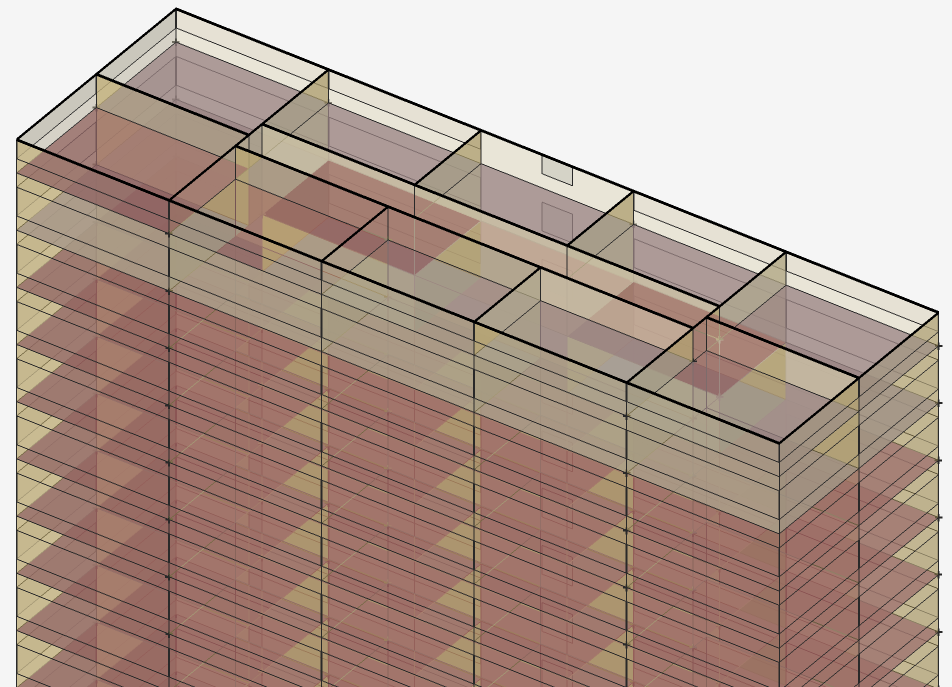
\includegraphics[width=0.5\textwidth]{figures/tab9-corte-19pav-v1.png}            \\ \hline
        Quantidade de zonas: 11                                                             & Quantidade de zonas: 11                                                           \\ \hline
        Área de projeção da torre: 843,75 m²                                                & Área de projeção da torre: 640,00 m²                                              \\ \hline
        Área da zona térmica “a”: 54,00 m²                                                  & Área da zona térmica “a”: 48,00 m²                                                \\ \hline
        Área da zona térmica “b”: 47,25 m²                                                  & Área da zona térmica “b”: 40,00 m²                                                \\ \hline
        Área da zona térmica “c+d”: 87,75 m²                                                & Área da zona térmica “c+d”: 88,00 m²                                              \\ \hline
        \makecell[l]{Largura do pavimento-tipo\\ (x): 16,00 m}                              & Largura do pavimento-tipo (x): 12,00 m                                            \\ \hline
        \makecell[l]{Comprimento do pavimento-\\tipo (y): 33,75 m}                          & \makecell[l]{Comprimento do pavimento-\\tipo (y): 40,00 m}                        \\ \hline
        \makecell[l]{Dimensões das aberturas\\ das zonas térmicas – N/S:\\ 6,70x1,51 m}     & \makecell[l]{Dimensões das aberturas das zonas\\ térmicas – N/S: 7,95x1,51 m}     \\ \hline
        \makecell[l]{Dimensões das aberturas\\ das zonas térmicas – L/O:\\ 7,95x1,51 m}     & \makecell[l]{Dimensões das aberturas das zonas\\ térmicas – L/O: 5,95x1,51 m}     \\ \hline
        \makecell[l]{Dimensões das aberturas\\ das zonas térmicas – circ.:\\ 1,49x1,51 m}   & \makecell[l]{Dimensões das aberturas das zonas\\ térmicas – circ.: 1,49x1,51 m}   \\ \hline
        \multicolumn{2}{l}{Dimensões das zonas térmicas – Pav. térreo e garagens: 40 x 25 m}                                                                                    \\ \hline
        \multicolumn{2}{l}{\makecell[l]{Dimensões das aberturas das zonas térmicas – Pav.\\ térreo e gar.: 39,95x1,51 m (N/S); 24,95x1,51 m (L/O)}}                             \\ \hline
    \end{tabular*}
    \begin{flushleft}
        \par \small Fonte: autor (2019).
    \end{flushleft}
    \label{tab:tabela9}
\end{table}

\noindent Foram propostas, na etapa de otimização, proteções solares horizontais para as aberturas, que servem como proteção à radiação solar direta e controle de iluminação natural em horários predeterminados – 9, 12 e 15 horas. Este controle de horários de incidência solar se deu pelo comprimento das proteções solares propostas. Esta solução foi adotada como estratégia passiva. Utilizou-se, também, a área para proteção solar como espaço para exploração de energia solar por meio de painéis fotovoltaicos sobre os elementos protetores, como exemplificado na Figura \ref{fig:figura11} \cite{Didone2014a}.
\begin{figure}[H]
    \centering
    \caption{\small Painéis fotovoltaicos sobre as proteções solares da fachada oeste e cobertura.}
    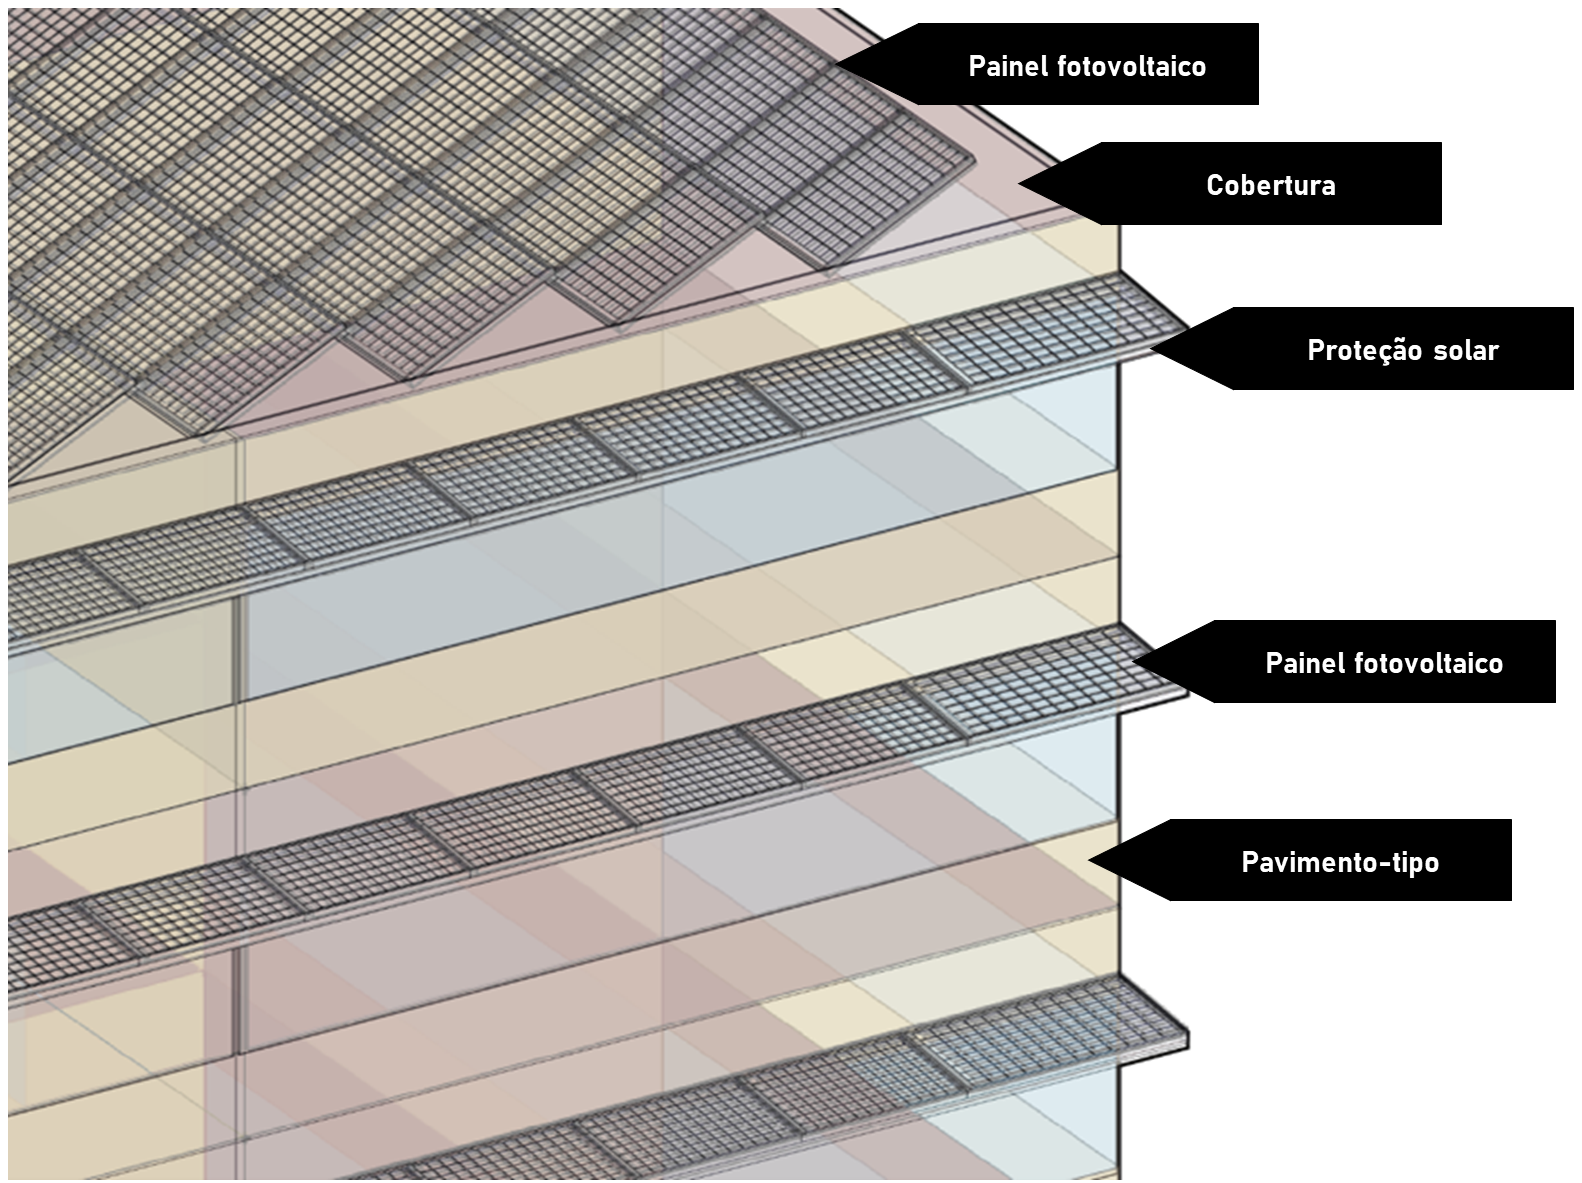
\includegraphics[width=0.9\textwidth]{figures/fig13-paineis pv.png}
    \begin{flushleft}
        \par \small Fonte: autor (2019).
    \end{flushleft}
    \label{fig:figura11}
\end{figure}

\subsubsection{Parâmetros arquitetônicos dos modelos genéricos}
\noindent A preparação para o início das simulações é precedida pela definição dos parâmetros arquitetônicos e das variáveis contidas em cada um destes. Com base no levantamento in loco e no referencial teórico, são inicialmente modificados os atributos arquitetônicos em três fases: envoltória, sistemas de iluminação e condicionamento de ar. As modificações foram implementadas de forma ordenada, a fim de evidenciar a influência de cada medida proposta no consumo final de energia elétrica da edificação genérica. As medidas propostas para analise por meio de simulação computacional estão apresentadas na Tabela \ref{tab:tabela10}.
\begin{table}[H]
    \centering
    \footnotesize
    \caption{\small Zonas térmicas dos modelos genéricos.}\vspace*{0.3cm}
    \begin{tabular*}{\columnwidth}{@{\extracolsep{\fill}}clcrl}\hline
        \multicolumn{2}{c}{\textbf{Parâmetros}}                                                                                              & \multicolumn{2}{c}{\textbf{Variáveis}}   & \textbf{Descrição}\\\hline
        \multirow{4}{*}{1}  & \multirow{4}{*}{Orientação Solar}                                                                              & a                  & 0°                  & \multirow{4}{*}{Orientação solar final da fachada principal.}\\
                            &                                                                                                                & b                  & 90°                 & \\
                            &                                                                                                                & c                  & 180°                & \\
                            &                                                                                                                & d                  & 360°                & \\\hline
        \multirow{4}{*}{2}  & \multirow{4}{*}{Vidro com baixo Fator Solar}                                                                   &                    &                     & \multirow{4}{*}{\makecell[l]{Foram simuladas duas situações aplicas aos\\
                                                                                                                                                                                         modelos genéricos: a primeira utilizando\\ o vidro
                                                                                                                                                                                         levantado in loco (a) e o modelo mais\\ eficiente
                                                                                                                                                                                         comercializado\\ no mercado brasileiro (b) (CB3E; ABIVIDRO, 2015).}}\\
                            &                                                                                                                & a                  & FS: 0,44            & \\
                            &                                                                                                                &                    &                     & \\
                            &                                                                                                                & b                  & FS: 0,16            & \\\hline
        \multirow{3}{*}{3}  & \multirow{3}{*}{\makecell[l]{Percentual de Área de Abertura\\ da Fachada Total – PAF\textsubscript{T}}}        & a                  & 30\%                & \multirow{3}{*}{\makecell[l]{As aberturas das fachadas foram definidas de\\
                                                                                                                                                                                            acordo com as indicações de programas de                                                                                                                                                                                             economia de energia como PROCEL EDIFICA e o\\
                                                                                                                                                                                            Advanced Energy Design Guide for Small to\\
                                                                                                                                                                                            Medium Office Buildings (Guia Avançado de\\
                                                                                                                                                                                            Planejamento Energético para Edificações de\\
                                                                                                                                                                                            Escritório de Pequeno e Médio Porte) da ASHRAE\\
                                                                                                                                                                                            (ASHRAE et al., 2014, 2019; FERRADOR FILHO;\\
                                                                                                                                                                                            AGUIAR; KNIESS, 2018).}}\\
                            &                                                                                                                & b                  & 50\%                & \\
                            &                                                                                                                & c                  & 80\%                & \\\hline
    \end{tabular*}
    \begin{flushleft}
        \par \small Fonte: autor (2019).
    \end{flushleft}
    \label{tab:tabela10}
\end{table}

\subsection{Simulações}
\noindent A etapa de simulação computacional foi determinada para averiguar o potencial das soluções propostas para os modelos genéricos e, desta maneira, verificar se os conceitos zero energy e near zero energy podem proporcionar resultados que minorem o consumo de energia das edificações criadas.\vspace*{0.3cm} \newline
\noindent Foram planejadas três etapas de simulações, conforme o Figura \ref{fig:figura14}, onde os resultados foram processados e verificado o nível de eficiência energética alcançado.
\begin{figure}[H]
    \centering
    \caption{Sequência de etapas de simulação.}
    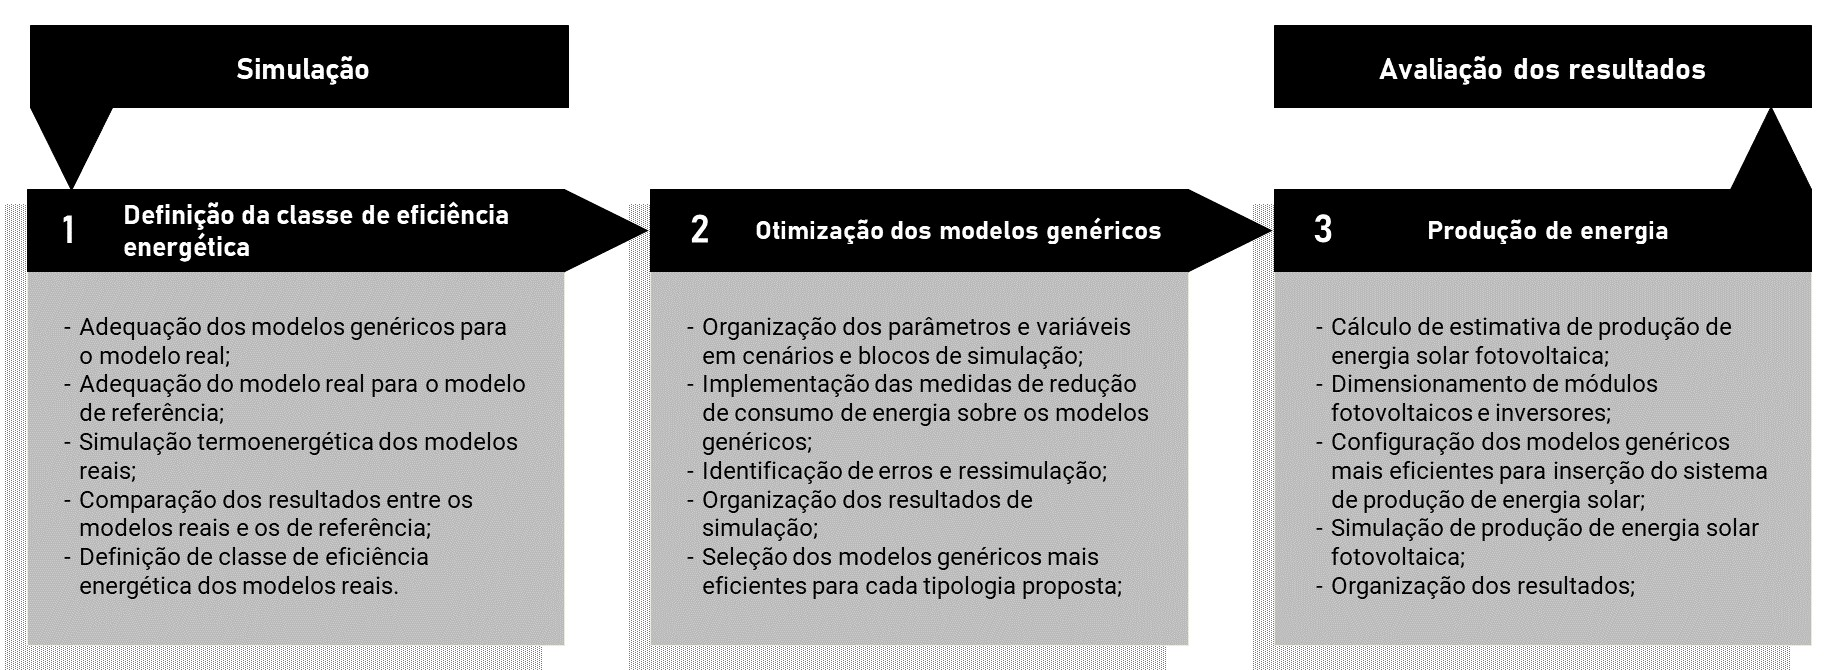
\includegraphics[width=1.0\textwidth]{figures/fig14-fluxograma-3.jpg}
    \begin{flushleft}
        \par \small Fonte: autor (2019)
    \end{flushleft}
    \label{fig:figura14}
\end{figure}
\subsubsection{Processo de modelagem}
\noindent Na etapa de modelagem foi realizada a composição dos modelos genéricos utilizando ferramentas computacionais de simulação de eficiência energética. Nesta fase foram configurados e ajustados os parâmetros incorporados aos modelos, como as características volumétricas, dados de desempenho dos equipamentos e soluções arquitetônicas.\vspace*{0.3cm} \newline
\noindent Trabalhos como o de Didoné \citeyear{Didone2014}, que realizou um estudo paramétrico de estratégias para edificações com balanço energético nulo no Brasil, utilizou o \textit{EnergyPlus} como principal ferramenta para simulação dos cenários termoenergéticos propostos. Carlo \citeyear{Carlo2008}, que desenvolveu uma metodologia de avaliação da eficiência energética para a envoltória de edificações não-residenciais, também utilizou essa ferramenta por reunir funções que auxiliariam na simulação de desempenho termoenergético e de parâmetros econômicos para verificação do consumo energético do modelo proposto.\vspace*{0.3cm} \newline
\noindent Outros autores aplicam o EnergyPlus por ser um software open source ou seja, software livre, amplamente utilizado pela comunidade cientifica e por reduzir os esforços no desenvolvimento de modelos matemáticos complexos para simulação de cenários termoenergéticos, auxiliando na otimização energética dos modelos propostos em estudo \cite{Vuong2015,Dahanayake2017,Shen2018,Kamal2019}.\vspace*{0.3cm} \newline
\noindent Portanto, a escolha da ferramenta mais apropriada para a modelagem dos parâmetros escolhidos como recurso ao processo de simulação da metodologia foi necessária. Seguindo a premissa de que a ferramenta deveria ser de livre acesso, ser validada em âmbito acadêmico e apresentar o maior volume de utilização em estudos de caso possível, como exemplificado na Figura \ref{fig:figure15}, foi adotado o software de simulação de energia em edificações \textit{EnergyPlus} 9.1.0-08d2e308bb \cite{U.S.DepartmentofEnergy-USDOE2011,Athienitis2015}.\vspace*{0.3cm} \newline
\noindent Da mesma forma, segundo Brackney et al. \citeyear{Brackney2018}, para facilitar o processo de configuração volumétrica e energética dos modelos, foram utilizadas ferramentas de suporte, que forneceram a interface entre o simulador e a ferramenta de modelagem. Estas ferramentas foram o \textit{SketchUp} 2017 trial version, versão 17.0.18899 \cite{TrimbleInc.2019}, para modelagem computacional tridimensional do edifício, e as extensões open-source para \textit{SketchUp, OpenStudio} v2.8.0, e a ferramenta de análise paramétrica \textit{Parametric Analysis Tool} – PAT.\vspace*{0.3cm} \newline
\begin{figure}[H]
    \centering
    \caption{\textit{Softwares} mais utilizados em simulação de eficiência de edificações.}
    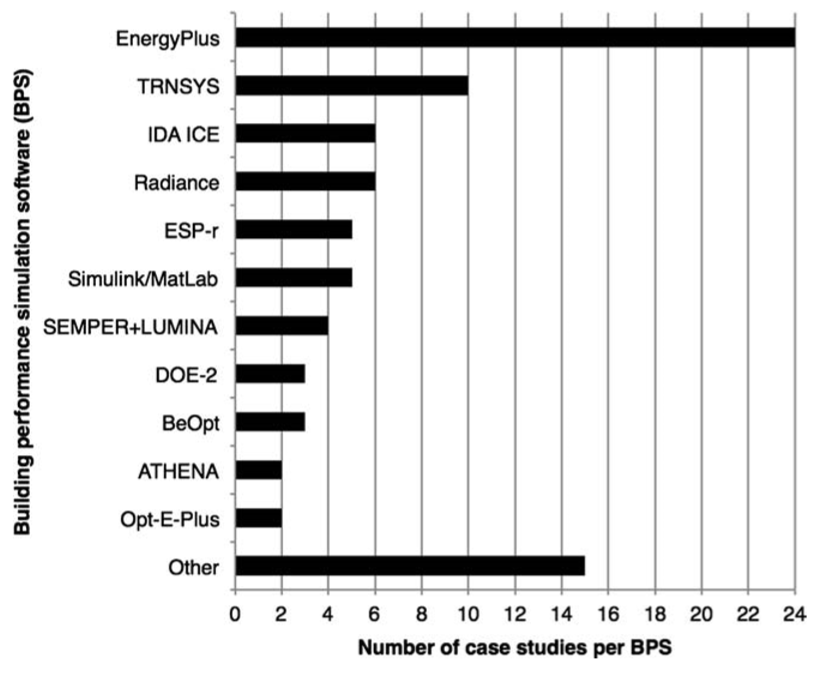
\includegraphics[width=0.8\textwidth]{figures/fig15-grafico-soft.png}
    \begin{flushleft}
        \par \small Fonte: adaptado de Athienitis; O’Brien (2015, tradução nossa).
    \end{flushleft}
    \label{fig:figure15}
\end{figure}
\noindent O início do processo de modelagem se dá pela configuração da volumetria utilizando as ferramentas internas do software de simulação computacional. Foram criadas as zonas térmicas das torres e dos pavimentos térreo e garagens, dimensões de aberturas externas e internas de cada zonas, assim como a quantidade de pavimentos-tipo das torres de cada modelo, definições de superfícies como piso, paredes e teto, e as áreas comuns de circulação horizontal e vertical, como ilustrado na Figura \ref{fig:figure16}.\vspace*{0.3cm} \newline
\noindent As janelas foram dimensionadas com cerca de 50\% do PAF\textsubscript{T}, com tamanhos variados, e com infiltração de ar padrão de 0,0003 m³/h/m² de área externa, como previamente definido na composição dos modelos genéricos. Todavia, as portas foram inseridas com medidas padrão reunidas em levantamento. Estas foram modeladas de acordo com as dimensões mais frequentes observadas no levantamento realizado, com 0,70 metros por 2,10 metros, e com infiltração de ar padrão da ferramenta de 0,0003 m³/h/m² de área de piso interna.\vspace*{0.3cm} \newline
\noindent Concluída a configuração da volumetria, inicia-se a composição dos dados do sítio onde o modelo genérico está implantado. Assim, foi inserido o arquivo climático de Vitória com os dados climáticos de 2018, no formato \textit{EnergyPlus Weather} – EPW, juntamente aos dias úteis do ano selecionado, no formato \textit{Design Conditions Design Days Data} – DDY \cite{InstitutoNacionaldeMetereologia-INMET2018}. Da mesma forma, foram configurados os dados da zona climática definida pela ASHRAE, 1A, similar à zona climática do recorte territorial.\vspace*{-0.25cm}
\begin{figure}[H]
    \centering
    \caption{Interface de configuração dos modelos genéricos no \textit{plug-in OpenStudio}.}
    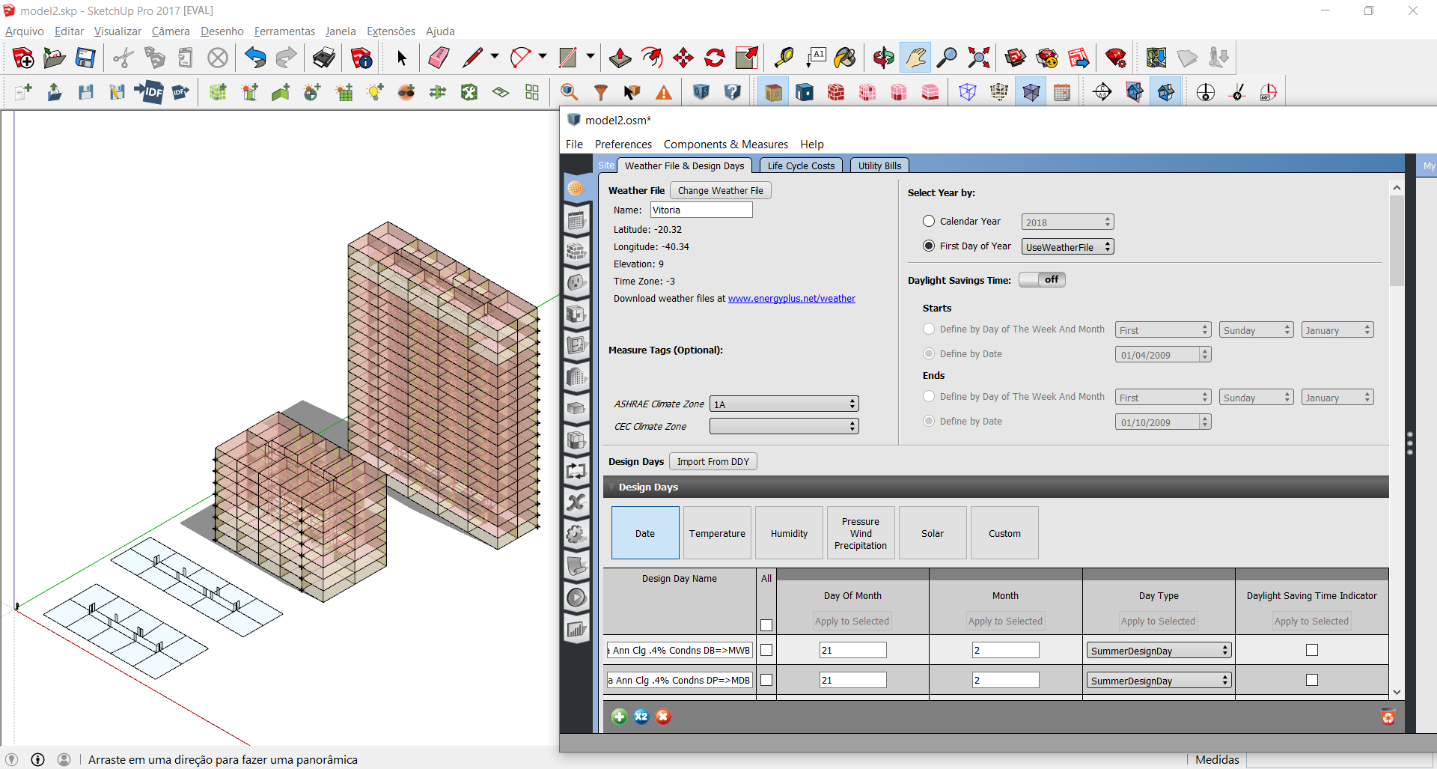
\includegraphics[width=0.8\textwidth]{figures/fig16-OS.png}
    \begin{flushleft}
        \par \small Fonte: autor, (2019).
    \end{flushleft}
    \label{fig:figure16}
\end{figure}
\noindent Concluída a etapa de geometrização e modelagem tridimensional da edificação, é dado início às configurações da envoltória, onde são atribuídos os dados de entrada característicos do empreendimento, como os valores de propriedades térmicas dos elementos construtivos, os dados de ocupação, por meio de schedules para vestimenta, horários de utilização dos ambientes, aberturas, iluminação e equipamentos, como exemplificado na Figura \ref{fig:figure17}.\vspace*{-0.25cm}
\begin{figure}[H]
    \centering
    \caption{Colagem da interface de inserção de dados das propriedades térmicas e de materiais.}
    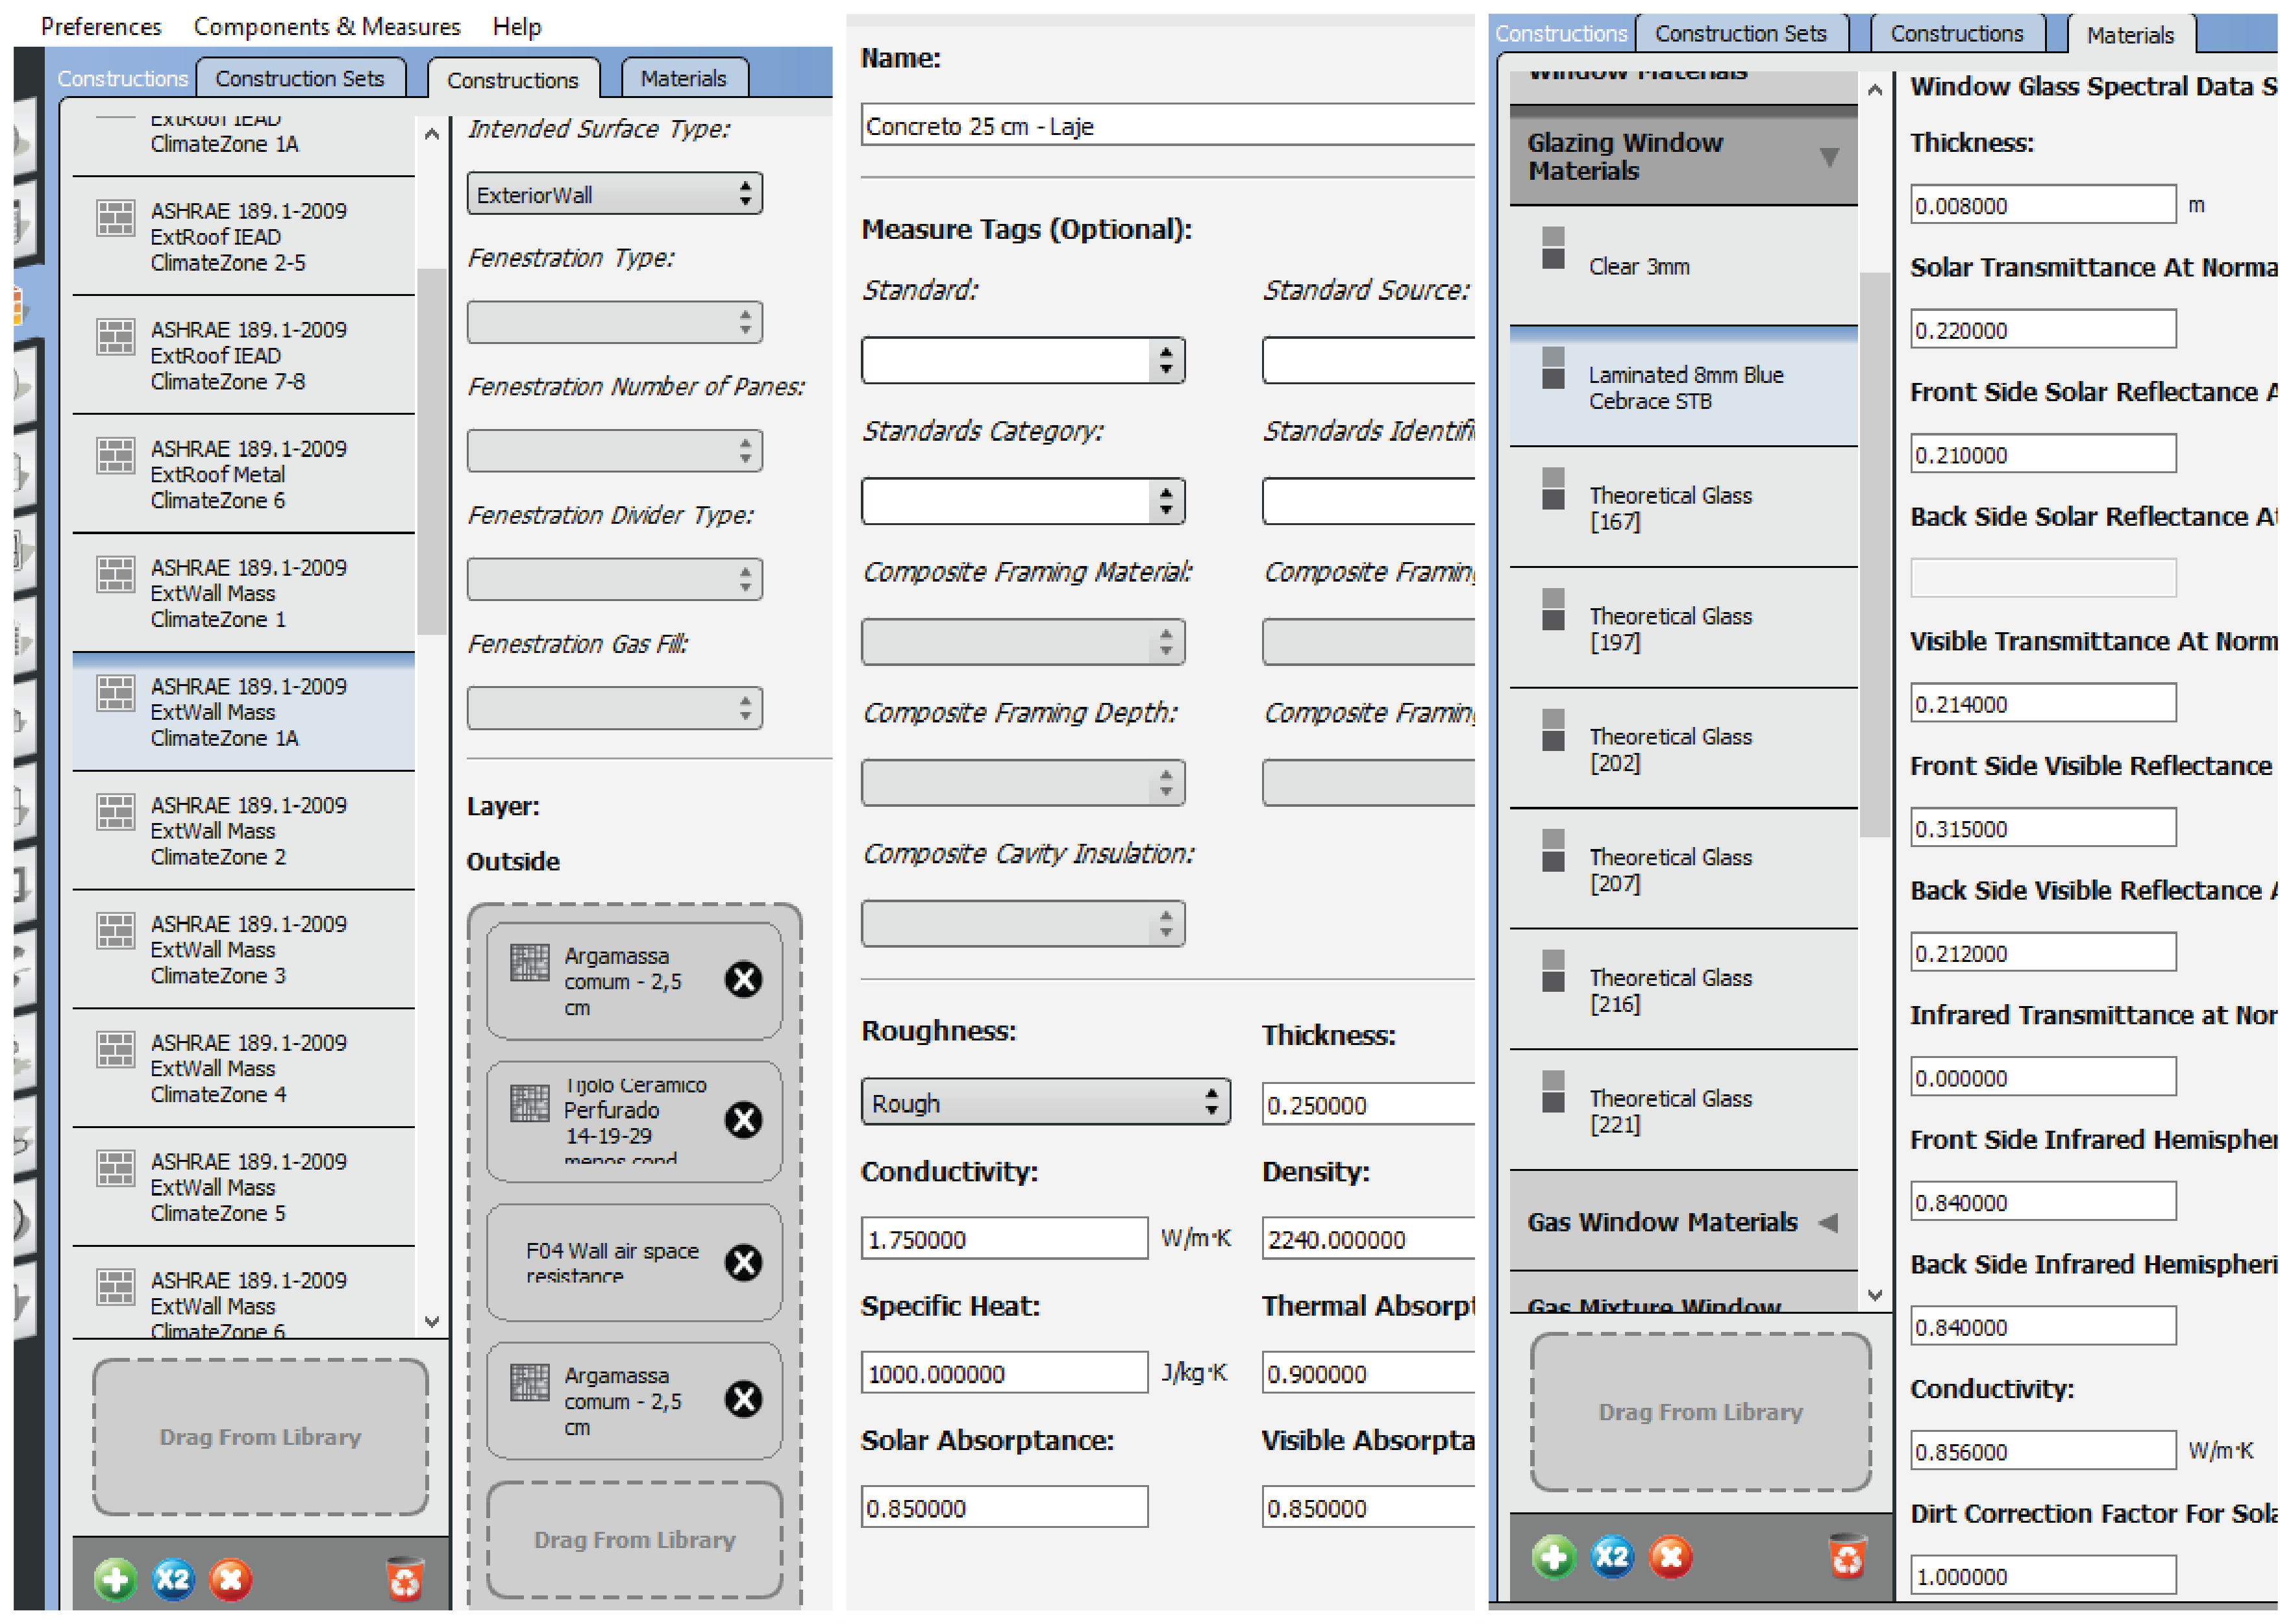
\includegraphics[width=0.8\textwidth]{figures/fig17-OS2.png}
    \begin{flushleft}
        \par \small Fonte: autor, (2019).
    \end{flushleft}
    \label{fig:figure17}
\end{figure}
\noindent Em seguida, foram configurados o sistema de condicionamento de ar, apresentado pela Figura \ref{fig:figure18}, segundo as características definidas para os modelos genéricos. Da mesma forma, foram implementadas medidas de parametrização das variáveis, medidas estas denominadas \textit{measures}, com a finalidade de reduzir o tempo total de processamento e simulação dos cenários. As \textit{measures} adotadas parametrizaram as mudanças de orientação solar, de componentes construtivos, de equipamentos de ar-condicionado e redução de carga de energia.\vspace*{-0.25cm}
\begin{figure}[H]
    \centering
    \caption{Interface de configuração dos sistemas de condicionamento de ar.}
    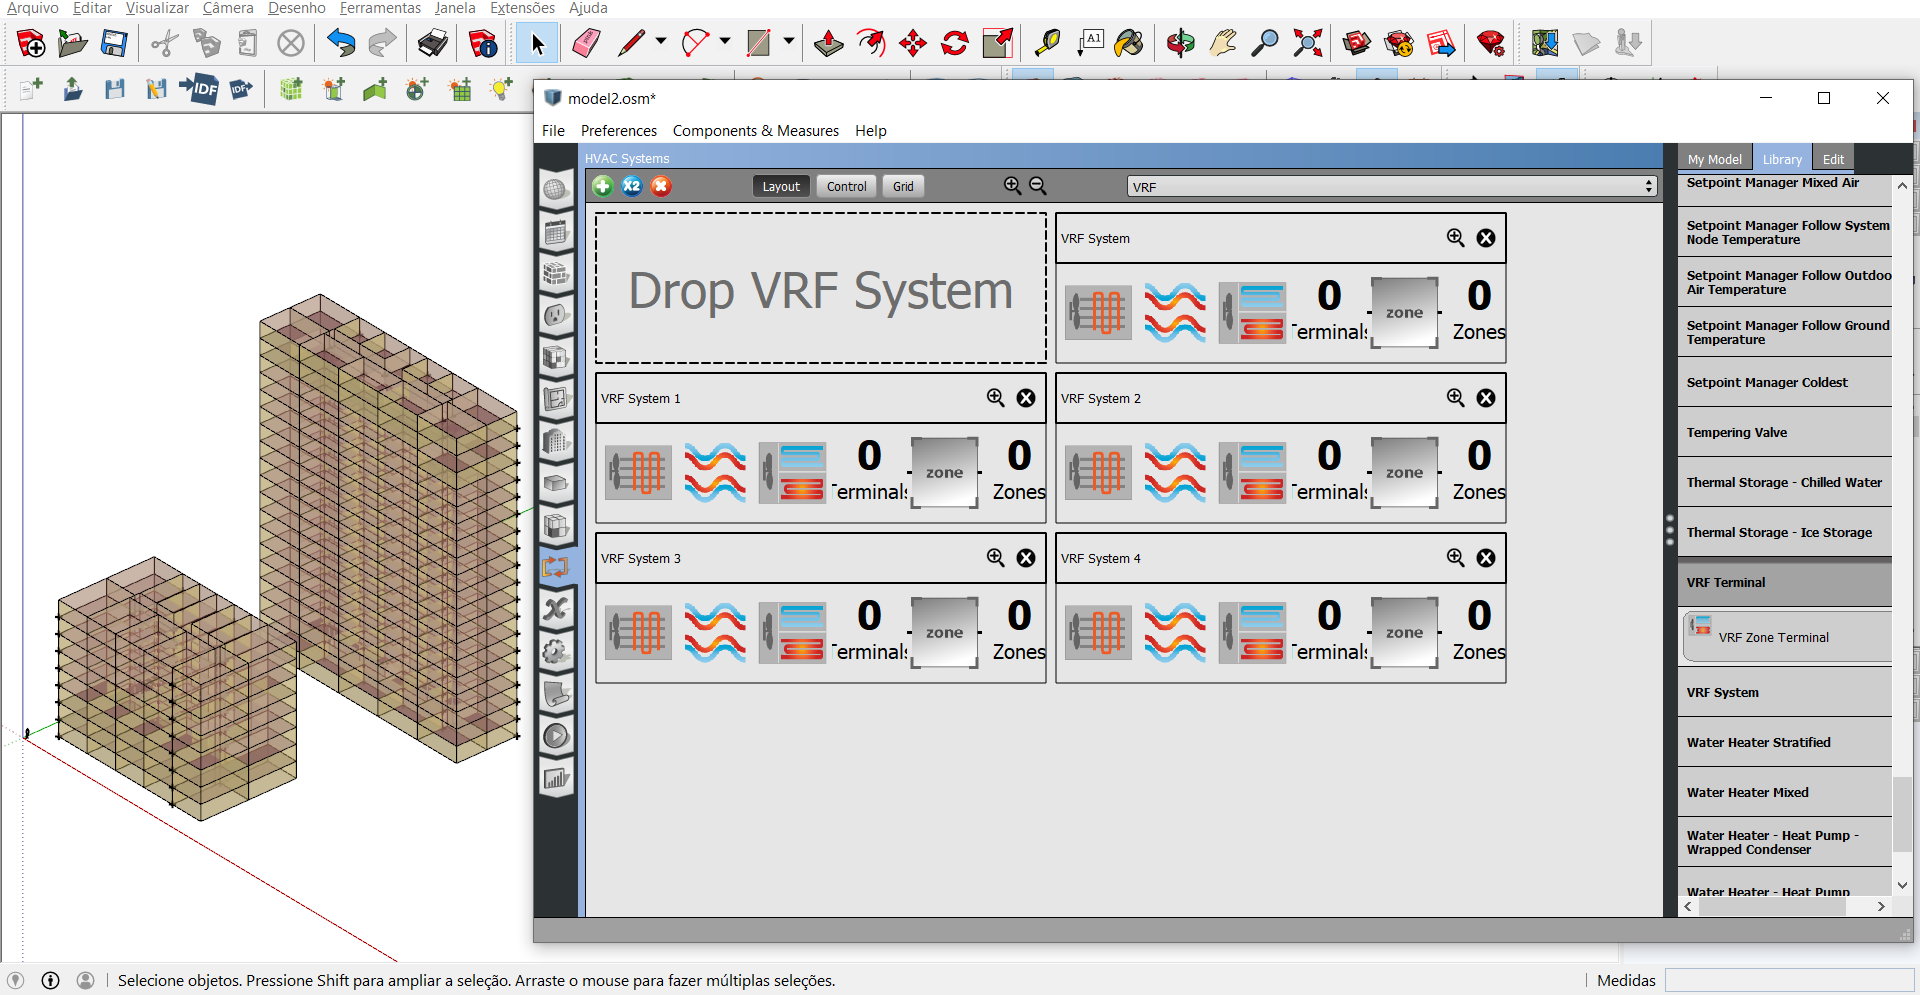
\includegraphics[width=0.85\textwidth]{figures/fig18-OS3.png}
    \begin{flushleft}
        \par \small Fonte: autor, (2019).
    \end{flushleft}
    \label{fig:figure18}
\end{figure}
\noindent Após as configurações de envoltória e sistemas concluídas, foram selecionadas as variáveis de saída relevantes à análise e feito a simulação teste, como exemplificado na Figura \ref{fig:figure19}. Desta forma os resultados foram concentrados nos dados de saída mais pertinentes, reduzindo o tempo total de simulação. Posteriormente, os modelos foram simplificados geometricamente, utilizando o recurso multiply, como abordado no subcapitulo sobre simplificação dos modelos genéricos \cite{Brackney2018}.\newline
\begin{figure}[H]
    \centering
    \caption{Saídas da simulaçãoem processo de finalização.}
    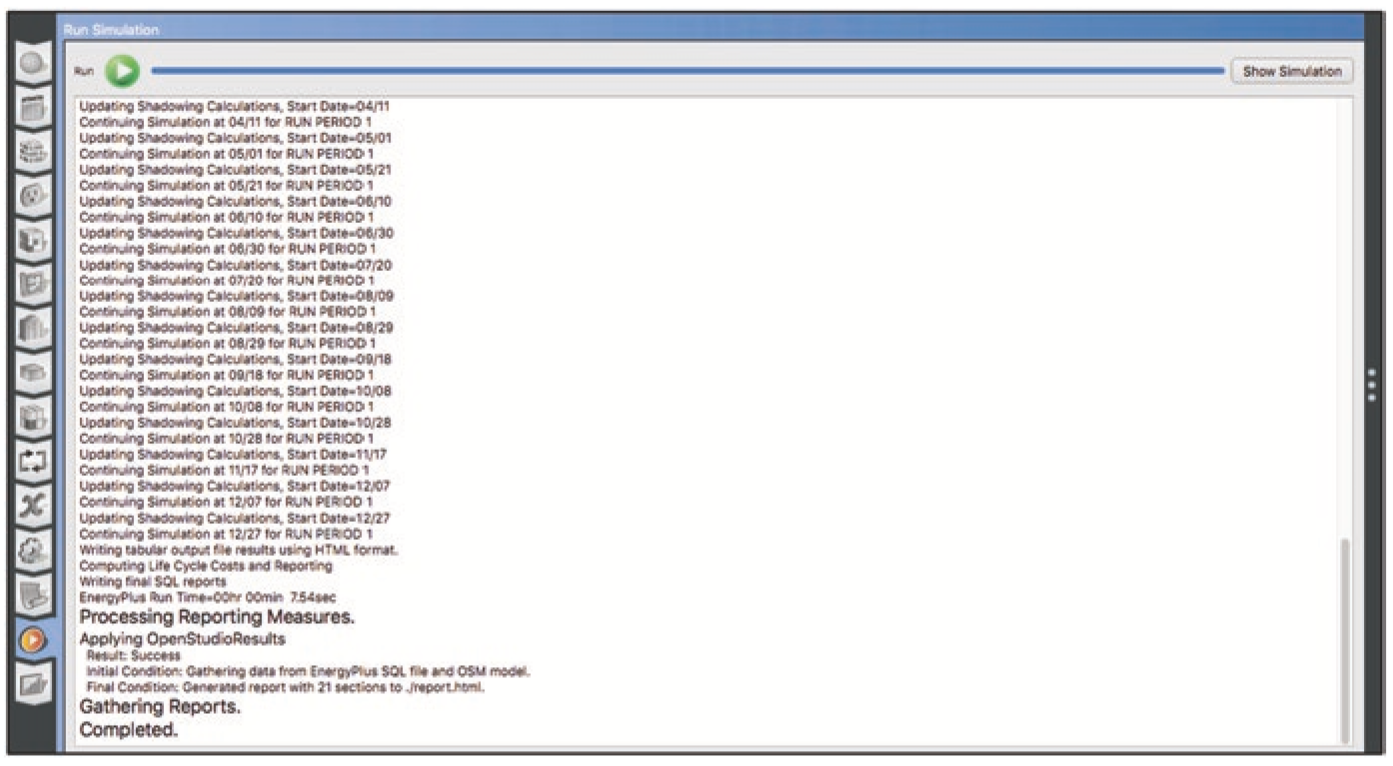
\includegraphics[width=0.9\textwidth]{figures/fig19-OS4.png}
    \begin{flushleft}
        \par \small Fonte: adaptado de Brackney et al. (2018).
    \end{flushleft}
    \label{fig:figure19}
\end{figure}
\subsubsection{Simplificação dos modelos genéricos e parametrização dos cenários}
\noindent A simulação energética e análise de um único cenário requer a utilização da ferramenta básica de modelagem, construção e revisão, que neste caso foi a ferramenta \textit{OpenStudio}. Entretanto, como este trabalho analisa vários cenários pertinentes a mais do que um modelo, foi necessária uma ferramenta mais robusta, que proporcionasse simulações simultâneas dos cenários construídos. Para esta finalidade, a ferramenta de parametrização PAT foi utilizada.\vspace*{0.3cm} \newline
\noindent Entretanto, um requisito necessário para que as simulações ocorram de forma simultânea e consumam pouco tempo de recurso computacional é a simplificação dos modelos. Esta simplificação consiste em reduzir o número de zonas térmicas a serem simuladas por meio da subtração de pavimentos que não sofrem influência da radiação solar e intempéries em uma edificação.\vspace*{0.3cm} \newline
\noindent Diante do exposto, o primeiro e o ultimo pavimento, juntamente ao pavimento intermediário a eles, foram mantidos, como apresentado na Figura \ref{fig:figure20}. Este recurso de redução de tempo de simulação é possível utilizando a função multiply disponibilizado pelo \textit{EnergyPlus} \cite{U.S.DepartmentofEnergy-USDOE2019}. Esta função tem como característica replicar os pavimentos selecionados a fim de multiplicar o número de zonas térmicas, área de piso e energia consumida pela carga interna virtualmente, substituindo as zonas térmicas modeladas e excluídas anteriormente.\newline
\begin{figure}[H]
    \caption{Modelos genéricos simplificados.}
    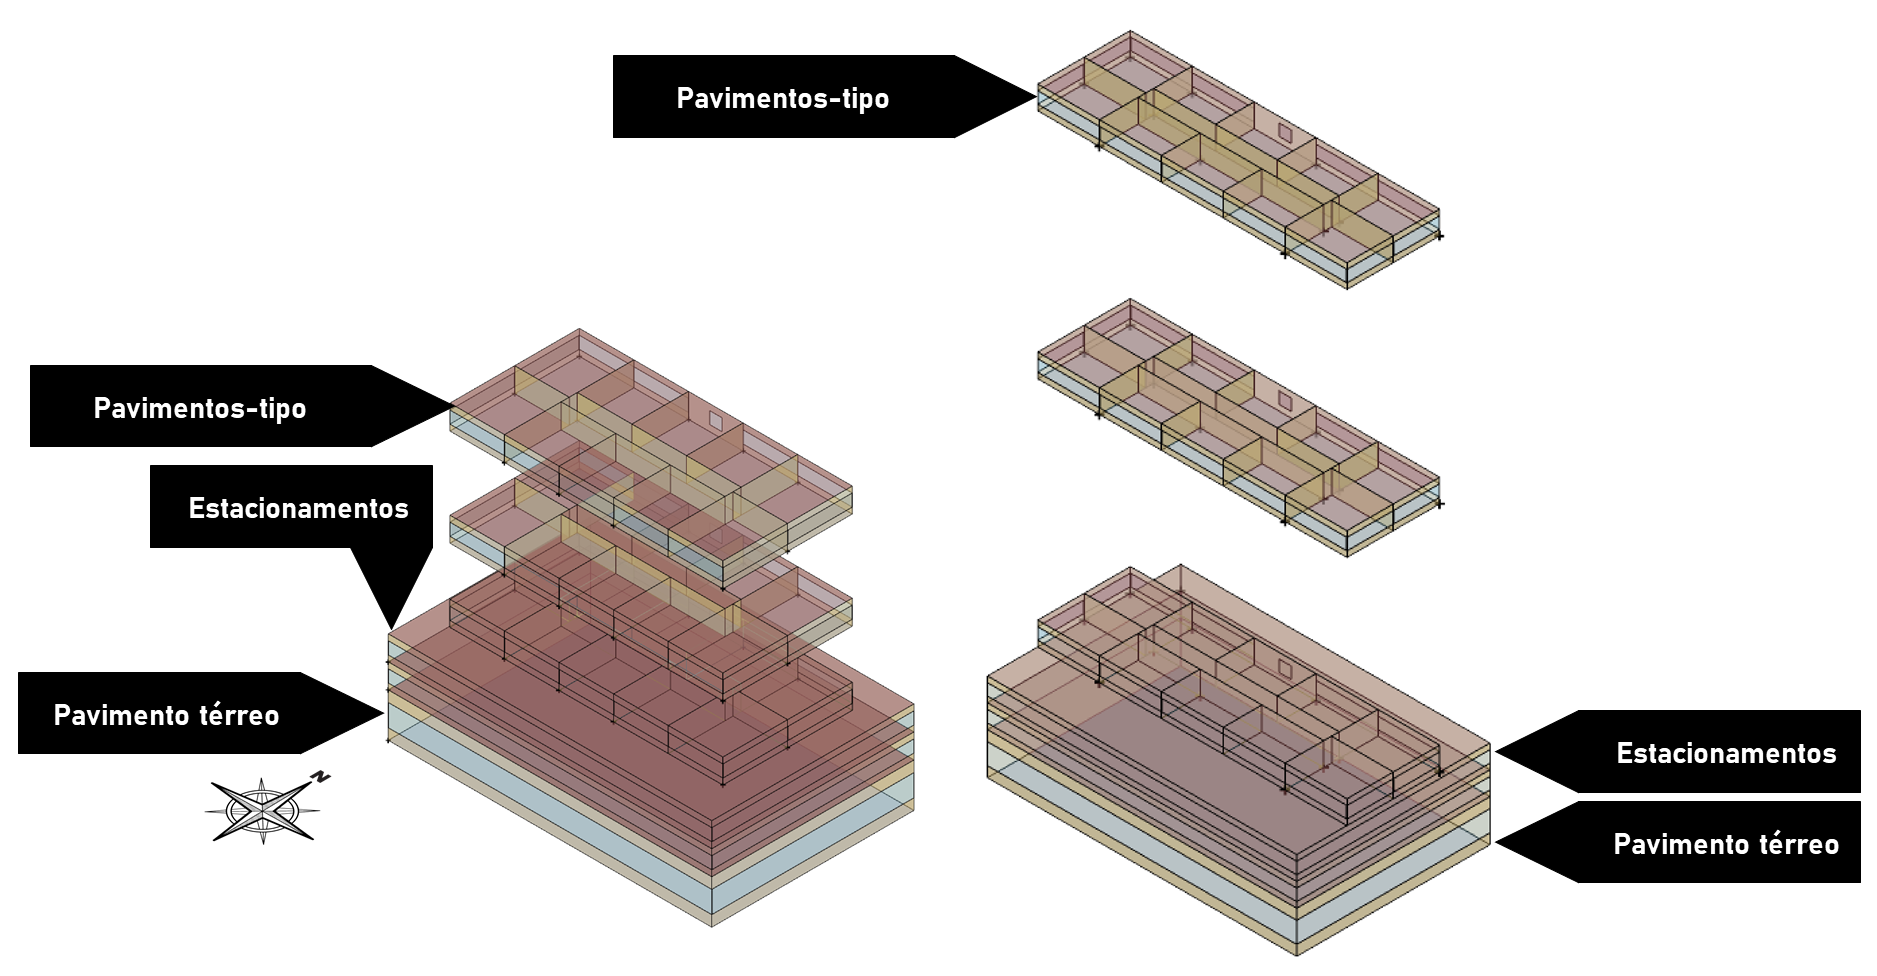
\includegraphics[width=1.0\textwidth]{figures/fig20-modelos.png}
    \begin{flushleft}
        \par \small Fonte: autor, (2019).
    \end{flushleft}
    \label{fig:figure20}
\end{figure}
\noindent Assim, a partir dos modelos simplificados, foram configurados os 368 cenários utilizando a ferramenta PAT, processo ilustrado pela Figura \ref{fig:figure21}. Desta forma, estes cenários que abrangem a etapa de otimização dos modelos genéricos foram simulados simultaneamente, reduzindo o tempo total de simulação e obtenção de resultados.\newline
\begin{figure}[H]
    \caption{Interface do \textit{Parametric Analysis Tool.}}
    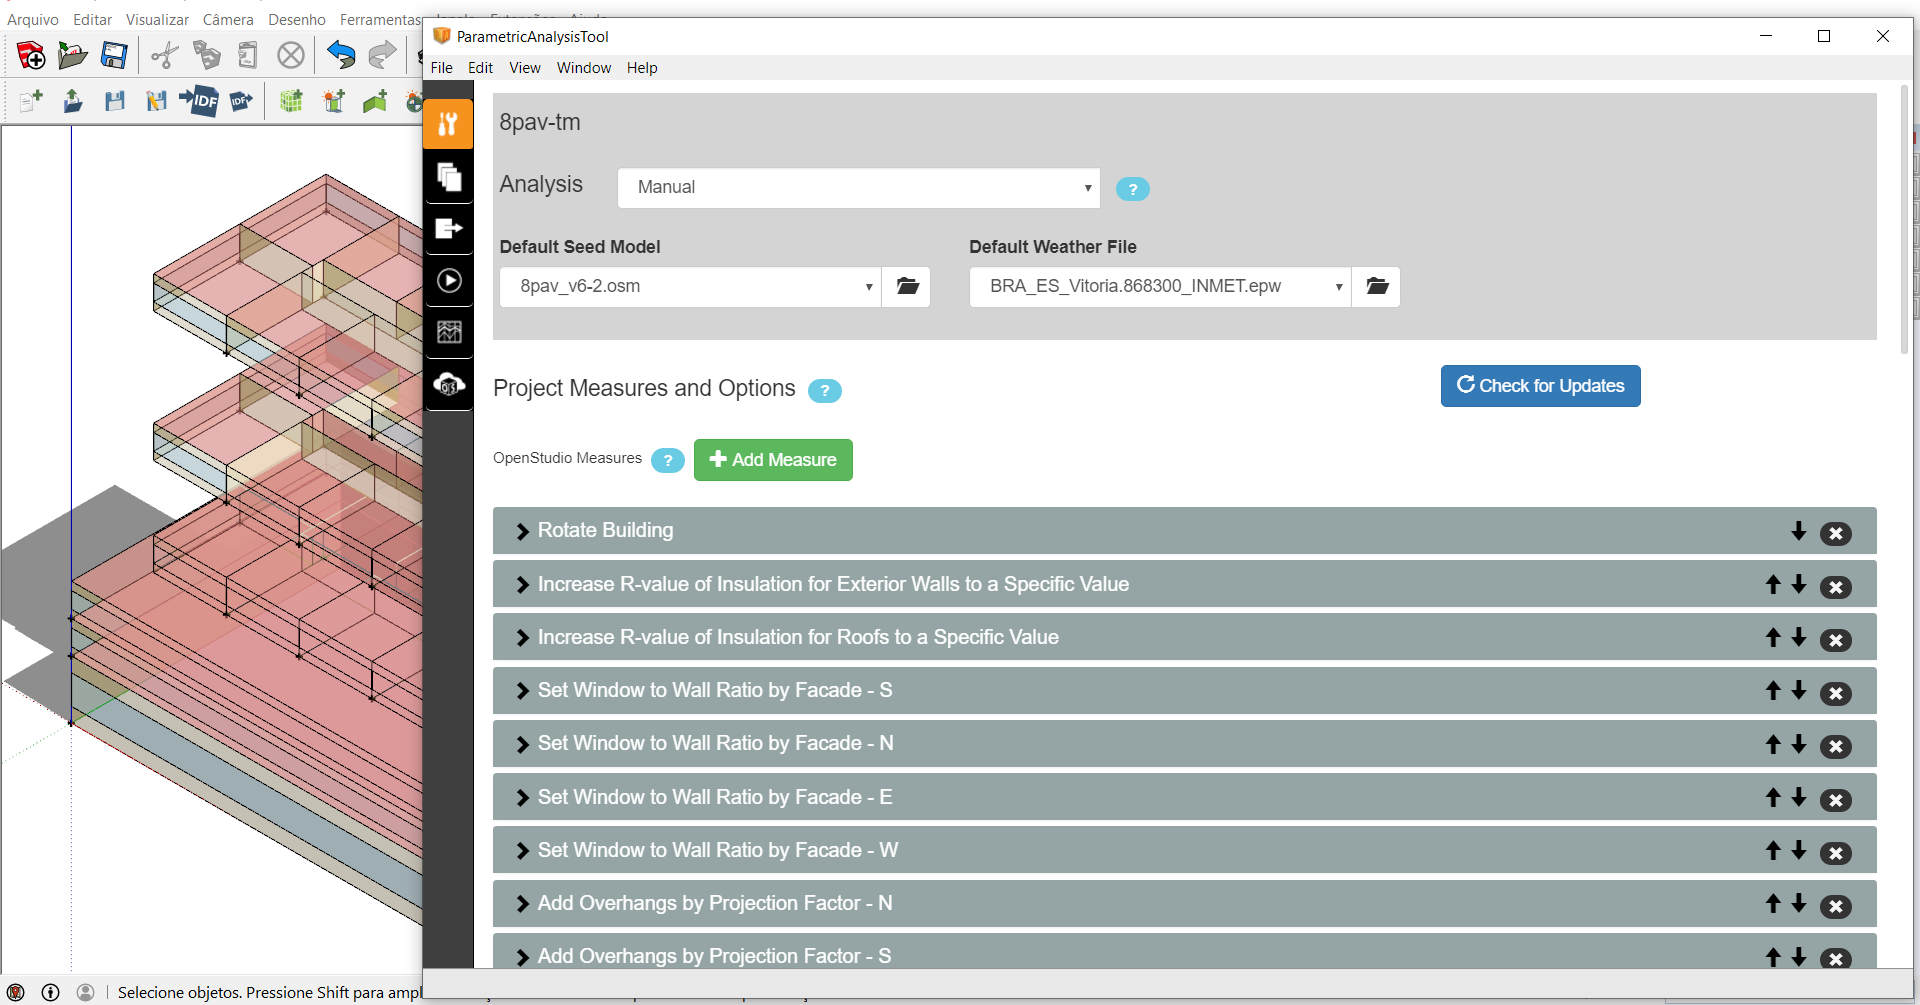
\includegraphics[width=1.0\textwidth]{figures/fig21-modelos.png}
    \begin{flushleft}
        \par \small Fonte: autor, (2019).
    \end{flushleft}
    \label{fig:figure21}
\end{figure}
\subsubsection{Processo de modelagem}
\noindent A partir da etapa de otimização, as informações reunidas sobre as estratégias passivas e ativas utilizadas neste trabalho serviram como base de dados para a configuração das measures no processo de simulações da PAT. As measures de estratégias ativas, como as medidas substituição do sistema de condicionamento de ar e de redução de carga de energia elétrica, foram executadas, respectivamente, no primeiro e no último bloco de simulações, compreendendo as reduções ativas de Intensidade de Uso de Energia e consumo final energético.\vspace*{0.3cm} \newline
\noindent Concomitantemente, os blocos de simulação implementados entre as medidas ativas de redução de energia englobaram as estratégias passivas, como mudança de PAF\textsubscript{T}, de componentes construtivos e alterações volumétricas e de orientação solar das fachadas. O processo de simulação dos cenários obedeceu a sequência de implementação das medidas para redução de consumo de energia disposta na Tabela \ref{tab:tabela13}.\vspace*{-0.1cm}
\begin{table}[H]
    \small
    \caption{\textit{Measures} utilizadas e os parâmetros correlacionados.}
    \begin{tabular}{llll}
    \hline
    \multicolumn{1}{c}{\textit{\textbf{Measure}}}                                                                                        & \multicolumn{1}{c}{\textbf{Parâmetro alvo}}                                                       & \multicolumn{2}{c}{\textbf{Inputs}}  \\ \hline
    \multirow{3}{*}{\makecell[l]{\textit{ZEGD VRF with DOAS;} \\ \textit{Add aPSZ-HP to each zone}}}                            & \multirow{3}{*}{\makecell[l]{Sistema de Condicionamento \\de Ar}}                                                 & a  & \textit{CAG/Fancoil}            \\
                                                                                                                                &                                                                                                   & b  & \textit{Split}                  \\
                                                                                                                                &                                                                                                   & c  & VRF                             \\ \hline
    \multicolumn{1}{l}{\multirow{4}{*}{\textit{Rotate Building}}}                                                               & \multicolumn{1}{l}{\multirow{4}{*}{Orientação solar}}                                             & a  & 0°                              \\
    \multicolumn{1}{l}{}                                                                                                        & \multicolumn{1}{l}{}                                                                              & b  & 90°                             \\
    \multicolumn{1}{l}{}                                                                                                        & \multicolumn{1}{l}{}                                                                              & c  & 180°                            \\
    \multicolumn{1}{l}{}                                                                                                        & \multicolumn{1}{l}{}                                                                              & d  & 270°                            \\ \hline
    \multirow{3}{*}{\makecell[l]{\textit{Increase R-value of Insulation for} \\ \textit{Exterior Walls to a Specific Value}}}   & \multirow{3}{*}{\makecell[l]{Transmitância térmica \\da parede da envoltória}}                    & a  & 2,46 W/m²K                      \\
                                                                                                                                &                                                                                                   & b  & 0,38 W/m²K                      \\
                                                                                                                                &                                                                                                   & c  & 0,32 W/m²K                      \\ \hline
    \multirow{3}{*}{\makecell[l]{\textit{Increase R-value of Insulation for} \\ \textit{Roofs to a Specific Value}}}            & \multirow{3}{*}{\makecell[l]{Transmitância térmica da \\cobertura}}                                               & a  & 3,73 W/m²K                      \\
                                                                                                                                &                                                                                                   & b  & 0,55 W/m²K                      \\
                                                                                                                                &                                                                                                   & c  & 0,53 W/m²K                      \\ \hline
    \multirow{3}{*}{\textit{Set Window to Wall Ratio by Facade}}                                                                & \multirow{3}{*}{\makecell[l]{Percentual de Área de \\Abertura da Fachada Total}}                  & a  & 30\%                            \\
                                                                                                                                &                                                                                                   & b  & 50\%                            \\
                                                                                                                                &                                                                                                   & c  & 80\%                            \\ \hline
    \multirow{3}{*}{\textit{Add overhangs by Projection Factor}}                                                                & \multirow{3}{*}{Proteção solar}                                                                   & a  & 20 cm                           \\
                                                                                                                                &                                                                                                   & b  & 50 cm                           \\
                                                                                                                                &                                                                                                   & c  & 100 cm                          \\ \hline
    \multirow{2}{*}{\textit{Reduce Lighting Loads by Percentage}}                                                               & \multirow{2}{*}{\makecell[l]{Medidas de Redução de Carga\\ de Energia Elétrica: Iluminação}}      & a  & n/a                             \\
                                                                                                                                &                                                                                                   & b  & 30\%                            \\ \hline
    \multirow{2}{*}{\textit{Reduce Equipment Loads by Percentage}}                                                              & \multirow{2}{*}{\makecell[l]{Medidas de Redução de Carga\\ de Energia Elétrica: Equipamentos}}    & a  & n/a                             \\
                                                                                                                                &                                                                                                   & b  & 30\%                            \\ \hline
    \multirow{2}{*}{\textit{Add, Remove or Replace Window}}                                                                     & \multirow{2}{*}{\makecell[l]{Vidros com transmitância \\térmica baixa}}                                           & a  & 0,44 W/m²K                      \\
                                                                                                                                &                                                                                                   & b  & 0,16 W/m²K                      \\ \hline
    \end{tabular}
    \begin{flushleft}
        \par \small Fonte: autor (2019).
    \end{flushleft}
    \label{tab:tabela13}
\end{table}
\vspace{-0.60cm} \noindent Com estas medidas, buscou-se atingir a eficiência energética necessária para o balanço energético dos modelos propostos, complementando a economia com produção de energia de fontes renováveis.

\subsubsection{Estimativa de produção de energia}
\noindent Para esta pesquisa, foi aplicado o sistema de produção de energia fotovoltaica, tanto por ser a mais usual nesse tipo de edificação como, também, pela complexidade da análise de custos para os outros sistemas, que inviabilizaria a conclusão da avaliação dentro do tempo disponível para o desenvolvimento do trabalho.\vspace*{0.3cm} \newline
\noindent A geração de energia solar foi avaliada a partir da área disponível para a implantação dos painéis fotovoltaicos. A área considerada para a produção de energia é constituída pela área de cobertura, de estacionamento, áreas opacas das fachadas e das proteções solares \cite{Didone2014}. Assim como a verificação de disponibilidade de áreas, os dados sobre a irradiação solar, radiação global difusa e anual, e a temperatura média anual de Vitória, extraídos do arquivo climático da cidade, foram considerados para a estimativa de produção de energia \cite{InstitutoNacionaldeMetereologia-INMET2018,Pereira2017}.\vspace*{0.3cm} \newline
\noindent A estimativa de produção de energia solar foi calculada com base no estudo de Palaoro \citeyear{Palaoro2019} sobre dimensionamento de sistema  fotovoltaico. Esta estimativa, necessária para suprir a demanda energética das edificações propostas, foi essencial para a obtenção  de dados para a simulação computacional de geração de energia solar fotovoltaica.\vspace*{0.3cm} \newline
\noindent Inicialmente foi calculada a energia de geração, E\textsubscript{geração}, como exposto na Equação \ref{eq:eq3}.
\begin{equation}\label{eq:eq3}
E_{geracao}=\frac{V_m}{30}
\end{equation}
\noindent Onde:\par
\setlength\parindent{1.5cm} E\textsubscript{geração} representa a quantidade de energia de geração, em kWh/mês; e\par
\setlength\parindent{1.5cm} V\textsubscript{m} é o valor médio de consumo da edificação.\par
\noindent Uma vez conhecida a energia de geração, foi estimada a quantidade de energia que cada modulo produziria diariamente, E\textsubscript{m}. De acordo com a Equação \ref{eq:eq4}, tem-se:
\begin{equation}\label{eq:eq4}
E_m=E_s \times A_m \times {\eta}_m
\end{equation}
\noindent Onde:\par
\setlength\parindent{1.5cm} E\textsubscript{m} é a quantidade estimada de energia produzida pelo modulo, expressa em Wh/dia;\par
\setlength\parindent{1.5cm} E\textsubscript{s} é a irradiação solar, em Wh/m²/dia;\par
\setlength\parindent{1.5cm} A\textsubscript{m} compreende a área da superfície do modulo, em m²; e\par
\setlength\parindent{1.5cm} \(\eta\)\textsubscript{m} é a eficiência do módulo.\par
\noindent Com as estimativas de geração de energia geral e por cada modulo diariamente, foram calculadas a  quantidade  de  módulos  necessários  para  atender  a  estimativa  de  geração  de  energia.  A quantidade de módulos, N\textsubscript{m}, é resultado da razão entre a quantidade de energia gerada, E\textsubscript{geração}, sobre a quantidade de energia gerada por cada modulo individualmente, E\textsubscript{m}. Desta forma, como expresso pela Equação \ref{eq:eq5}, tem-se que:
\begin{equation}\label{eq:eq5}
N_m=\frac{E_{geracao}}{E_m}
\end{equation}
\noindent Os módulos e inversores foram pesquisados de acordo com as dimensões e especificações estimadas por meio das equações demonstradas neste capítulo, como apresentado na Tabela \ref{tab:tabela14}. O sistema fotovoltaico indicado ao cenário dos modelos genéricos foi de porte comerciais, dada a demanda de energia calculada. Os inversores foram dimensionados de forma a aproveitar a potência máxima nominal dos módulos, evitando o subdimensionamento e inadequação entre inversores e módulos durante o processo de geração de energia do sistema fotovoltaico.
\subsubsection{Simulação de geração de energia}
\noindent A simulação de produção de energia solar foi realizada por meio da ferramenta PVsyst, versão v6.8.1 \cite{Cronemberger2012}. Esta ferramenta foi utilizada por disponibilizar a análise de desempenho e dimensionamento do sistema de produção de energia solar necessário para empreendimentos do porte da edificação proposta nesta pesquisa. Complementarmente a ferramenta, foi feito um levantamento dos módulos fotovoltaicos comercializados no Brasil de acordo com a aplicação destes componentes sobre a envoltória, como módulos monocristalinos de silício, m-Si, e filme fino de Telúrio de Cádmio, Cd-Te \cite{Didone2014,Werneck2017,Sorgato2018}. Estas tecnologias foram escolhidas por serem indicadas para a aplicação sobre as superfícies horizontais, como a cobertura e o estacionamento, e verticais, como as fachadas.\newline
\begin{table}[H]
    \small
    \caption{Módulos fotovoltaicos utilizados e a áreadisponível para implantação.}
    \begin{tabular}{lllll}
    \hline
    \multicolumn{2}{c}{\multirow{2}{*}{\textbf{Características}}}                                                                                   & \multicolumn{3}{c}{\textbf{Modelo genérico de 8 pavimentos}}                                                                                                                   \\ \cline{3-5} 
    \multicolumn{2}{c}{}                                                                                                                            & \multicolumn{1}{c}{\makecell[c]{\textbf{Cobertura} \\\textbf{e estacionamento}}}   & \multicolumn{1}{c}{\makecell[c]{\textbf{Proteção} \\ \textbf{solar}}}            & \multicolumn{1}{c}{\textbf{Fachada}}                      \\ \hline
    \multicolumn{1}{c}{\parbox[t]{2mm}{\multirow{8}{*}{\rotatebox[origin=c]{90}{\textbf{Módulo}}}}} & Módulo                                        & \multicolumn{1}{c}{\makecell[c]{SunPower \\SPR-E20-435-COM}}              & \multicolumn{1}{c}{\makecell[c]{SunPower \\SPR-E20-435-COM}}           & \multicolumn{1}{c}{\makecell[c]{First Solar \\FS-4122-2}}                 \\
    \multicolumn{1}{c}{}                                                                            & Tecnologia                                    & \multicolumn{1}{c}{m-SI}                                  & \multicolumn{1}{c}{m-SI}                               & \multicolumn{1}{c}{Cd-Te}                                 \\
    \multicolumn{1}{c}{}                                                                            & Potência máx. (Wp)                            & \multicolumn{1}{c}{435}                                   & \multicolumn{1}{c}{435}                                & \multicolumn{1}{c}{122,5}                                 \\
    \multicolumn{1}{c}{}                                                                            & Tensão máx. (V)                               & \multicolumn{1}{c}{324}                                   & \multicolumn{1}{c}{648}                                & \multicolumn{1}{c}{376}                                   \\
    \multicolumn{1}{c}{}                                                                            & \makecell[l]{Potência Nominal \\- STC (kWp)}  & \multicolumn{1}{c}{150}                                   & \multicolumn{1}{c}{100,92}                             & \multicolumn{1}{c}{274,22}                                \\
    \multicolumn{1}{c}{}                                                                            & Nº de módulos                                 & \multicolumn{1}{c}{345}                                   & \multicolumn{1}{c}{232}                                & \multicolumn{1}{c}{2238}                                  \\
    \multicolumn{1}{c}{}                                                                            & Eficiência (\%)                               & \multicolumn{1}{c}{19}                                    & \multicolumn{1}{c}{19}                                 & \multicolumn{1}{c}{17}                                    \\
    \multicolumn{1}{c}{}                                                                            & Área ocupada (m²)                             & \multicolumn{1}{c}{746}                                   & \multicolumn{1}{c}{501}                                & \multicolumn{1}{c}{1612}                                  \\ \hline
    \parbox[t]{2mm}{\multirow{5}{*}{\rotatebox[origin=c]{90}{\textbf{Inversor}}}}                   & Modelo                                        & \multicolumn{1}{c}{\makecell[c]{Fronius \\International \\IG Plus 150 V-3}} & \multicolumn{1}{c}{\makecell[c]{Fronius \\International \\ECO 25.0-3-S}} & \multicolumn{1}{c}{\makecell[c]{Fronius International \\IG Plus 150 V-3}} \\
                                                                                                    & Nº de inversores                              & \multicolumn{1}{c}{10}                                    & \multicolumn{1}{c}{6}                                  & \multicolumn{1}{c}{14}                                    \\
                                                                                                    & \makecell[l]{Potência máx. \\total (kWac)}    & \multicolumn{1}{c}{120}                                   & \multicolumn{1}{c}{50}                                 & \multicolumn{1}{c}{84}                                    \\
                                                                                                    & Tensão de entrada (V)                         & \multicolumn{1}{c}{230-500}                               & \multicolumn{1}{c}{580-850}                            & \multicolumn{1}{c}{230-500}                               \\
                                                                                                    & Eficiência (\%)                               & \multicolumn{1}{c}{97,9}                                  & \multicolumn{1}{c}{97,9}                               & \multicolumn{1}{c}{97,9}                                  \\ \hline
    \multicolumn{2}{c}{\multirow{2}{*}{\textbf{Características}}}                                   & \multicolumn{3}{c}{\textbf{Modelo genérico de 19 pavimentos}}                                                                                                                   \\ \cline{3-5} 
    \multicolumn{2}{c}{}                                                                            & \multicolumn{1}{c}{\makecell[c]{\textbf{Cobertura} \\\textbf{e estacionamento}}}                          & \multicolumn{1}{c}{\makecell[c]{\textbf{Proteção} \\ \textbf{solar}}}            & \multicolumn{1}{c}{\textbf{Fachada}}                      \\ \hline
    \multicolumn{1}{c}{\parbox[t]{2mm}{\multirow{8}{*}{\rotatebox[origin=c]{90}{\textbf{Módulo}}}}} & Módulo                                        & \multicolumn{1}{c}{\makecell[c]{SunPower \\SPR-E20-435-COM}}              & \multicolumn{1}{c}{\makecell[c]{SunPower \\SPR-E20-435-COM}}           & \multicolumn{1}{c}{\makecell[c]{First Solar \\FS-4122-2}}                 \\
    \multicolumn{1}{c}{}                                                                            & Tecnologia                                    & \multicolumn{1}{c}{Si-mono}                                  & \multicolumn{1}{c}{Si-mono}                               & \multicolumn{1}{c}{Cd-Te}                                 \\
    \multicolumn{1}{c}{}                                                                            & Potência máx. (Wp)                            & \multicolumn{1}{c}{435}                                   & \multicolumn{1}{c}{435}                                & \multicolumn{1}{c}{122,5}                                 \\
    \multicolumn{1}{c}{}                                                                            & Tensão máx. (V)                               & \multicolumn{1}{c}{324}                                   & \multicolumn{1}{c}{648}                                & \multicolumn{1}{c}{376}                                   \\
    \multicolumn{1}{c}{}                                                                            & \makecell[l]{Potência Nominal \\- STC (kWp)}  & \multicolumn{1}{c}{150}                                   & \multicolumn{1}{c}{243,40}                             & \multicolumn{1}{c}{479,70}                                \\
    \multicolumn{1}{c}{}                                                                            & Nº de módulos                                 & \multicolumn{1}{c}{345}                                   & \multicolumn{1}{c}{560}                                & \multicolumn{1}{c}{3917}                                  \\
    \multicolumn{1}{c}{}                                                                            & Eficiência (\%)                               & \multicolumn{1}{c}{19}                                    & \multicolumn{1}{c}{19}                                 & \multicolumn{1}{c}{17}                                    \\
    \multicolumn{1}{c}{}                                                                            & Área ocupada (m²)                             & \multicolumn{1}{c}{746}                                   & \multicolumn{1}{c}{745}                                & \multicolumn{1}{c}{2820}                                  \\ \hline
    \parbox[t]{2mm}{\multirow{5}{*}{\rotatebox[origin=c]{90}{\textbf{Inversor}}}}                   & Modelo                                        & \multicolumn{1}{c}{\makecell[c]{Fronius \\International \\IG Plus 150 V-3}} & \multicolumn{1}{c}{\makecell[c]{Fronius \\International \\ECO 25.0-3-S}} & \multicolumn{1}{c}{\makecell[c]{Fronius \\International \\IG Plus 150 V-3}} \\
                                                                                                    & Nº de inversores                              & \multicolumn{1}{c}{10}                                    & \multicolumn{1}{c}{13}                                  & \multicolumn{1}{c}{22}                                    \\
                                                                                                    & \makecell[l]{Potência máx. \\total (kWac)}    & \multicolumn{1}{c}{162}                                   & \multicolumn{1}{c}{125}                                 & \multicolumn{1}{c}{250}                                    \\
                                                                                                    & Tensão de entrada (V)                         & \multicolumn{1}{c}{580-850}                               & \multicolumn{1}{c}{580-850}                            & \multicolumn{1}{c}{580-850}                               \\
                                                                                                    & Eficiência (\%)                               & \multicolumn{1}{c}{97,9}                                  & \multicolumn{1}{c}{97,9}                               & \multicolumn{1}{c}{97,7}                                  \\ \hline
                                                                                                    &                                               &                                                           &                                                        &                                                          
    \end{tabular}
    \begin{flushleft}
        \par \small Fonte: autor, (2019).
    \end{flushleft}
    \label{tab:tabela14}
    \end{table}
    \vspace{-0.60cm} \noindent Foram simulados cenários de acordo com a aplicação da proteção solar proposta assim como para cada PAF\textsubscript{T}. Todavia, com a dimensão dos equipamentos de proteção solar definida, de acordo com a Tabela 14, foi levantada a quantidade de área disponível para a implantação dos módulos fotovoltaicos, segundo a incidência de irradiação solar sobre a superfície dos modelos e da latitude de Vitória.\newline
    \noindent Foi considerado 70\% da área do segundo pavimento de estacionamento para a instalação da estrutura de suporte aos módulos fotovoltaicos. Esta estrutura desempenharia a função de cobertura para os veículos, uma vez que esta área é descoberta e apresenta áreas de manobra e acesso as vagas. Além disso, a inclinação dos módulos foi configurada da seguinte forma:
    \begin{itemize}
        \item A área da cobertura e estacionamento com inclinação de 20°;
        \item Os módulos da fachada com 90° por estarem instalados nas superfícies opacas da fachada, perpendiculares ao piso; e
        \item Os módulos instalados nas proteções solares com inclinação de 5°, a fim de aumentar a incidência solar sobre os módulos sem comprometer a fachada, dificultar o deposito de sedimentos e facilitar a manutenção do sistema.
    \end{itemize}
    \noindent Para atingir a máxima produção de energia solar fotovoltaica, foi proposto o deslocamento das torres dos modelos para maior exposição da área de estacionamento à radiação solar, como exemplificado na Figura \ref{fig:figure22}. Vale lembrar que Plano Diretor vigente sobre o recorte territorial não limita a cobertura da área de cobertura do estacionamento em relação aos lotes circundantes, uma vez que a área em questão não está ao nível do térreo, permitindo a implementação das coberturas com painéis fotovoltaicos.\vspace*{-0.2cm}
    \begin{figure}[H]
        \caption{Deslocamento de torres dos modelos genéricos sobre as áreas de estacionamento. O volume tracejado demonstra a posição original da torre antes do deslocamento.}
        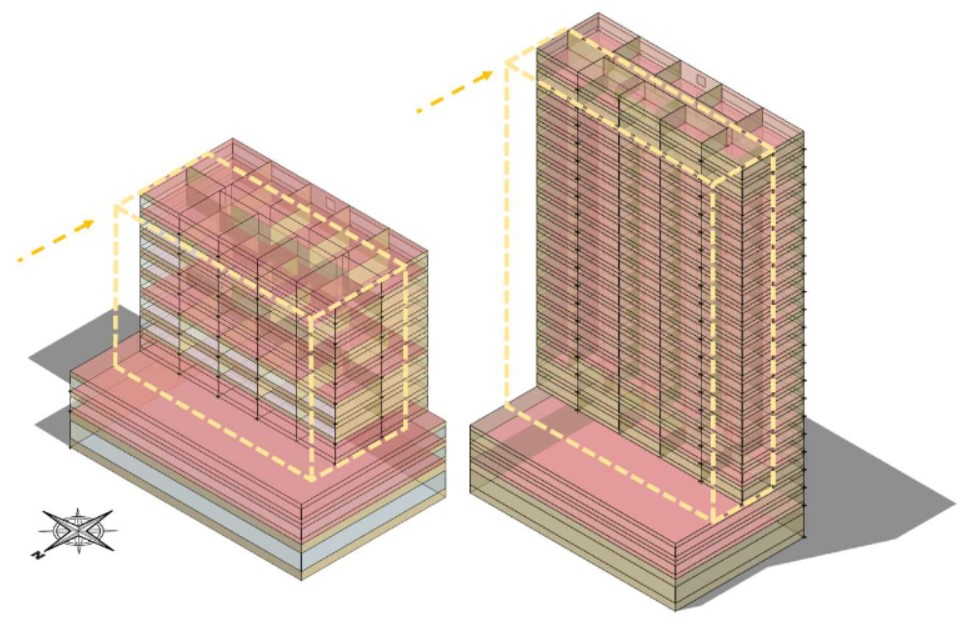
\includegraphics[width=1.0\textwidth]{figures/fig22-modelos.jpg}
        \begin{flushleft}
            \par \small Fonte: autor, (2019).
        \end{flushleft}
        \label{fig:figure22}
    \end{figure}
\subsection{Avaliação de resultados}
\noindent Foram examinados os aspectos econômicos da implantação das tecnologias propostas para produção de energia das edificações, sendo avaliados os cenários onde os modelos genéricos de 8 e 19 pavimentos foram mais eficientes, relacionando o custo de implementação das modificações propostas. Além do custo, foi avaliada a influência dos parâmetros estudados sobre os modelos genéricos, de forma estatística, por meio da análise de sensibilidade entre as variáveis adotadas e os resultados alcançados.
\subsubsection{Análise de viabilidade econômica}
\noindent A mudança de equipamentos de iluminação e condicionamento de ar, instalação de protetores solares  e  os  custos  da  implantação  de  tecnologias  de  produção  de  energia  estão  entre  as modificações propostas para a redução do consumo de energia elétrica. Os custos de instalação e manutenção do sistema de produção de energia fotovoltaica foi obtida por meio de consulta a empresas  locais  que  comercializam  painéis  fotovoltaicos,  além  de  publicações  acadêmicas recentes acerca do tema.\newline
\noindent A análise de viabilidade financeira dos cenários simulados foi realizada por meio do cálculo do Valor Presente Líquido – VPL, e payback \cite{CasarottoFilho2010,Puccini2011}.  Segundo Puccini \citeyear{Puccini2011}, VPL é definido como a diferença entre o valor investido em um tempo inicial \(t=0\), e o valor presente da riqueza  futura  gerada  pelo  projeto.  Esta  definição  pode  ser  expressa pela Equação \ref{eq:eq6}.
\begin{equation}\label{eq:eq6}
    VPL_{mod gen}=V_r - Investimento Total
\end{equation}
\noindent Juntamente  ao  VLP,  será  calculado  o  Valor  de  Retorno, V\textsubscript{r},  e  desta  forma,  foram  definidos parâmetros que compõe esta análise como o período do investimento, a tarifa de energia elétrica e  a  Taxa  Mínima  de  Atratividade,  com  base  nos  dados  sobre  a  inflação  média  lançados  pelo Instituto Brasileiro de Geografia e Estatística – IBGE. Estes parâmetros estão descritos na Equação \ref{eq:eq7} \cite{Puccini2011}.\newline
\begin{equation}\label{eq:eq7}
    V_r=A \times \left\{\frac{1-\left[\frac{1}{(1+i)^n}\right]}{i}\right\}
\end{equation}
\noindent Onde:\par
\setlength\parindent{1.5cm} V\textsubscript{r} é o valor de retorno;\par
\setlength\parindent{1.5cm} A é o recebimento anual sucessivo;\par
\setlength\parindent{1.5cm} \textit{n} representa o período definido do investimento; e\par
\setlength\parindent{1.5cm} \textit{i} é a taxa mínima de atratividade do investimento.\par
\noindent Nesse sentido, definem-se as seguintes condições:\par
\begin{itemize}
    \item Se \(VPL>0\), o investimento produziu ganhos – projeto aceito;
    \item Se \(VPL=0\), o investimento e os ganhos foram equilibrados – projeto aceito; e
    \item Se \(VPL<0\), o investimento foi maior que os ganhos – projeto a rejeitar.
\end{itemize}
\noindent A partir da validade do projeto, seja ele com produção de lucro ou equilibrado entre investimento e ganhos, deve ser avaliado o tempo de retorno do investimento – payback. Esta análise verifica se o somatório das parcelas anuais é igual ao investimento inicial \cite{CasarottoFilho2010}. Para tal, define-se então que o payback pode ser representado pela Equação \ref{eq:eq8}.\newline
\begin{equation}\label{eq:eq8}
    \textit{Payback}=\frac{\textit{Investimento inicial}}{\textit{Pagamento por período}}
\end{equation}
\noindent Após a conclusão da análise de viabilidade econômica, são apresentados os dados resultantes da aplicação da metodologia  proposta e discussão acerca das possibilidades observadas por meio desta apresentação de resultados.
\subsubsection{Análise de variáveis sobre consumo e produção de energia}
\noindent A análise do impacto das variáveis foi aplicada sobre os resultados com o intuito de evidenciar o nível de influência destas sobre o consumo final de energia dos modelos genéricos. Esta análise foi baseada no processamento de dados provenientes dos resultados de simulação. A aplicação sequencial e ordenada das medidas de redução de consumo de energia na etapa de otimização facilitou a plotagem de gráficos e a compreensão dos dados de saída para cada bloco de simulação.\newline
\noindent Assim como a análise da etapa de otimização, os resultados de geração de energia foram submetidos à verificação de erro e desvio padrão, como descrito nas Equação \ref{eq:eq9} e Equação \ref{eq:eq10}, com a finalidade de corrigir os resultados para imprecisões de medição e depreciação da performance do sistema estudado.\newline
\begin{equation}\label{eq:eq9}
    S=\sqrt{\frac{\sum_{i=1}^{n}(X_i-\bar{X}^2)}{n-1}}
\end{equation}
\noindent Onde:\par
\setlength\parindent{1.5cm} \textit{S} é o desvio padrão normal;\par
\setlength\parindent{1.5cm} X\textsubscript{i} é a \textit{i-ésima} observação da amostral;\par
\setlength\parindent{1.5cm} \textit{X} é a média da amostra;\par
\setlength\parindent{1.5cm} \textit{n} é o tamanho da amostra;\par
\begin{equation}\label{eq:eq10}
    ep=\frac{S}{\sqrt{n}}
\end{equation}
\noindent Onde:\par
\setlength\parindent{1.5cm} \textit{ep} é o erro padrão da amostra;\par
\setlength\parindent{1.5cm} \textit{S} é o desvio padrão da amostra;\par
\setlength\parindent{1.5cm} \textit{n} é o tamanho da amostra;\par

\end{onehalfspace}
\section{Resultados e discussão}
\noindent Neste capítulo são apresentados os resultados obtidos sobre o potencial de balanço energético nulo e quase nulo para as edificações propostas. No primeiro momento, os modelos foram classificados segundo a classe de eficiência energética disposta pelo INI-C, seguidos das otimizações que resultaram na análise de impacto das medidas implementadas. Após as otimizações foram avaliados os sistemas de produção de energia solar fotovoltaica propostos, e a capacidade de geração de energia anual.\vspace*{0.3cm} \newline
\noindent Verificou-se que a otimização e as estratégias ativas e passivas proporcionaram as condições necessárias para o balanço energético dos modelos. Ao final das simulações de consumo e produção de energia, foi analisada a viabilidade econômica das soluções propostas. Esta análise mostrou condições econômicas favoráveis de implantação do sistema de produção de energia proposto aos modelos.  Estes dados foram expressos em gráficos e tabelas a fim de facilitar a compreensão dos resultados alcançados.
\subsection{Classificação de desempenho energético dos modelos genéricos}
\noindent Para a determinação da classe de eficiência energética dos modelos genéricos, segundo a metodologia descrita pelo INI-C, é exigida a comparação entre dois cenários definidos como modelo real e o modelo de referência. Desta forma, foram configurados os cenários para a identificação do consumo total de energia térmica, elétrica e de energia primária, como descrito no capítulo 3. Como resultado, foi constatada a baixa eficiência energética dos modelos, como exposto na Tabela \ref{tab:tabela15}.
\begin{table}[H]
    \centering
    \small
    \caption{Resultados da classificação de desempenho energético dos modelos genéricos iniciais.}
\begin{tabular}{llll}
    \hline
    \textbf{Descrição}                                    & \textbf{Variável}      & \makecell[c]{\textbf{Modelo} \\\textbf{Real}} & \makecell[c]{\textbf{Modelo de} \\\textbf{Referência}}  \\ \hline
    \multicolumn{4}{c}{\textbf{Classe de desempenho energético - modelo de 8 pavimentos}}                                                  \\ \hline
    \makecell[l]{Consumo total de \\energia térmica}                      & CTEt (kWh/ano)         & 418197               & 443178                         \\
    \makecell[l]{Consumo total de \\energia elétrica - CTEe}              & CTEe (kWh/ano)         & 1086401              & 1142584                        \\
    \makecell[l]{Consumo de energia primária \\da edificação selecionada} & \makecell[l]{CEP real/ref \\(kWh/ano)} & 2198258,3            & 2315630,2                      \\ \hline
    \multicolumn{3}{l}{Etiqueta da edificação real}                                                       & \multicolumn{1}{c}{\textbf{D}} \\ \hline
    \multicolumn{4}{c}{\textbf{Classe de desempenho energético - modelo de 19 pavimentos}}                                                 \\ \hline
    \makecell[l]{Consumo total de \\energia térmica}                      & CTEt (kWh/ano)         & 1115708              & 1137261                        \\
    \makecell[l]{Consumo total de \\energia elétrica - CTEe}              & CTEe (kWh/ano)         & 2643097              & 2676556                        \\
    \makecell[l]{Consumo de energia primária \\da edificação selecionada} & \makecell[l]{CEP real/ref \\(kWh/ano)} & 5456234              & 5533476,7                      \\ \hline
    \multicolumn{3}{l}{Etiqueta da edificação real}                                                       & \multicolumn{1}{c}{\textbf{D}} \\ \hline
    \end{tabular}
    \begin{flushleft}
        \par \small \vspace{0.1cm} Fonte: autor (2019).
    \end{flushleft}
    \label{tab:tabela15}
\end{table}
\noindent O desempenho enérgico dos modelos ampara a necessidade de otimização, quanto as características construtivas e de sistemas das edificações, para tornar as condições de performance propícias ao balanço energético.
\subsection{Impacto das variáveis sobre o consumo anual de energia elétrica}
\noindent A etapa de otimização possibilitou visualizar a influência das variáveis sobre o consumo anual final das edificações para cada cenário definido. Os resultados da implementação das medidas ativas de redução de consumo de energia, disponíveis nos Apêndices deste trabalho, demonstraram maior peso entre as variáveis de estratégia ativa, pertencentes aos blocos de simulação 2, 3 e 9, e passivas, formadas pelos blocos de simulação 1, e de 4 a 10, como exposto nos Gráficos 4 e 5.\vspace*{0.3cm} \newline
\noindent Nota-se que as variáveis de estratégias ativas reduziram significativamente o consumo anual, com curvas de queda expressivas, direcionando a média de consumo para baixo, posicionando alguns cenários abaixo da média linear, como observado entre os blocos de simulação 1 ao 7 do Gráfico 4. Este comportamento se estende até o bloco de simulação 7 no modelo de 19 pavimentos, desempenho demonstrado no Gráfico 5. Os blocos de simulação compostos por variáveis passivas apresentaram constância de forma e estreitamento ao longo do avanço das implementações das medidas. O estreitamento gradativo da amplitude da curva de consumo final anual em ambos os resultados sugere que o avanço cumulativo das medidas de mitigação de consumo é importante para o sucesso do processo de adequação da edificação ao conceito \textit{Zero Energy}.\vspace*{0.3cm} \newline
\noindent A tendência ascendente das curvas de consumo, a partir do bloco de simulação 4, é causada pela alteração do PAF\textsubscript{T}, partindo da menor razão, de 30\%, até alcançar a maior razão entre área de fachada e área de aberturas envidraçadas, com 80\%. Esta medida aponta a importância da adoção de aberturas menores, em torno de 30\%, para a melhor relação entre o PAF\textsubscript{T} e o consumo energético da edificação.\vspace*{0.3cm} \newline
\noindent Os gráficos serviram como instrumento de tomada de decisão acerca da seleção dos melhores cenários para a etapa de simulação de geração de energia solar fotovoltaica. Além disso, os gráficos facilitaram a visualização da importância de cada estratégia adotada para o balanço energético nulo das edificações avaliadas. A leitura dos gráficos pode ser feita da seguinte forma:
\begin{itemize}
    \item Os gráficos consistem em evidenciar o impacto das medidas adotadas no consumo da edificação. Para tal, foi definida a comparação entre o desempenho dos modelos por meio do percentual de redução de consumo de energia entre as edificações. Esta comparação desconsidera a escala dos gráficos, já que ambos correspondem a edificações de portes diferentes, e considera o comportamento das medidas aplicadas por meio de análise das curvas de consumo;
    \item Os pontos na cor laranja representam cada cenário montado, os quais variam entre 4 conjuntos de implementação sequencial de medidas de redução de energia. Cada conjunto de cenários pertencentes aos 10 blocos de simulação estão definidos e representados nos Gráficos 4 e 5;
    \item As curvas em verde representam a tendência de aumento ou redução de consumo de 
    energia entre a simulação dos cenários;
    \item Como a mudança entre os tipos de vidro avaliados, foi necessário realizar novas simulações de todos os blocos anteriores a esta medida, sendo essa etapa representada pelas curvas acentuadas entre conjuntos de cenários, como, por exemplo, observado na curva entre os cenários 12 e 13 do bloco de simulação 10, na página 93.            
\end{itemize}
\noindent A redução de consumo provocada pela implementação de equipamentos e iluminação mais eficientes atinge o patamar de 22,48\% de redução global, assim como o sistema de arrefecimento, com 34,78\% para o modelo de 19 pavimentos. As reduções no modelo de 8 pavimentos foram tênues, da ordem de 16,09 e 16,66\%, respectivamente, para os sistemas de arrefecimento, e equipamentos e iluminação, como observado na Figura 21.\vspace*{0.3cm} \newline
\noindent Entretanto, cabe mencionar que o desempenho de controle térmico do sistema Split para o modelo de 19 pavimentos, nos cenários iniciais, provocou maior consumo de energia em relação aos dois outros sistemas de arrefecimento avaliados, CAG e VRF, em 22,73\%. Após a implementação do vidro mais eficiente, houve redução do consumo em cerca de 24,91\%, superando ligeiramente em performance o sistema CAG. Em contraste a esta observação do Split para o modelo de 19 pavimentos, este sistema obteve comportamento semelhante ao sistema VRF para a edificação de 8 pavimentos, com considerável performance e redução de consumo de energia. O \textit{Split} apresentou controle satisfatório das médias de temperatura de conforto das zonas térmicas. A diferença de desempenho dos sistemas de condicionamento de ar entre os dois modelos pode ser atribuída a diferença de carga térmica entre as edificações, onde o modelo de 8 pavimentos apresenta menor carga térmica e menor exposição à radiação solar em comparação ao modelo de 19 pavimentos.\vspace*{0.3cm} \newline
\begin{figure}[H]
    \centering
    \rotatebox{90}{
        \begin{minipage}{\textheight}
            \caption{Consumo \textit{versus} medidas do modelo genérico de 8 pavimentos.}
            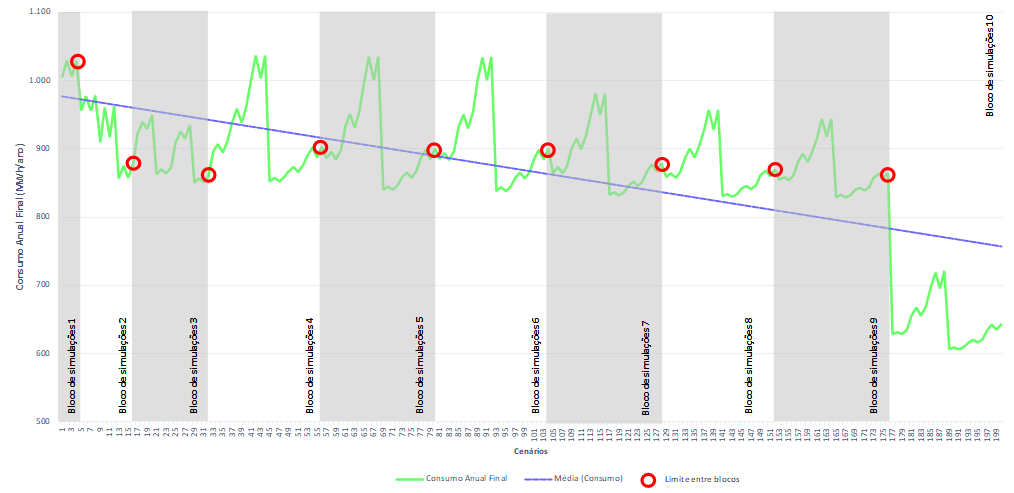
\includegraphics[width=1.0\textwidth]{figures/result/fig23-grafico4.png}
            \begin{flushleft}
                \par \small Fonte: autor, (2020). Legenda: Bloco de simulações 1 a 3 – Blocos com implementação do vidro, orientações solares e sistemas de condicionamento de ar; Bloco de simulações 4 –Bloco com implementação das variações de PAF\textsubscript{T}; Bloco de simulações 5 e 6 – Blocos com implementação de paredes e coberturas; Bloco de simulações 7 e 8 e 9 – Blocos com implementação das proteções solares; Bloco de simulações 10 – Blocos com implementação das medidas de redução de carga.
            \end{flushleft}
            \label{fig:figure23}
        \end{minipage}
    }
\end{figure}
\pagebreak

\begin{figure}[H]
    \centering
    \rotatebox{90}{
        \begin{minipage}{\textheight}
            \caption{Consumo \textit{versus} medidas do modelo genérico de 19 pavimentos.}
            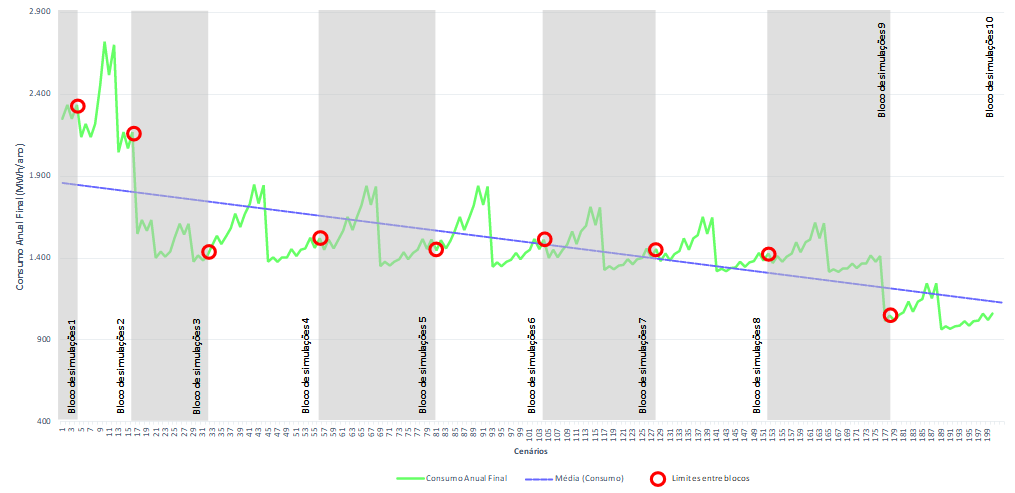
\includegraphics[width=1.0\textwidth]{figures/result/fig24-grafico5.png}
            \begin{flushleft}
                \par \small Fonte: autor, (2020). Legenda: Bloco de simulações 1 a 3 – Blocos com implementação do vidro, orientações solares e sistemas de condicionamento de ar; Bloco de simulações 4 –Bloco com implementação das variações de PAF\textsubscript{T}; Bloco de simulações 5 e 6 – Blocos com implementação de paredes e coberturas; Bloco de simulações 7 e 8 e 9 – Blocos com implementação das proteções solares; Bloco de simulações 10 – Blocos com implementação das medidas de redução de carga.
            \end{flushleft}
            \label{fig:figure24}
        \end{minipage}
    }
\end{figure}
\pagebreak
\noindent Como os vidros foram utilizados em todos os cenários, a importância da variável se torna mais visível quando comparado com todas as variáveis, assim como apresentado na Figura \ref{fig:figure25}. Verifica-se que, ao longo das implementações de medidas passivas, a influência é reduzida de 14,40\% para 4,00\%, conforme observado anteriormente nos blocos de simulação 3 e 4.\vspace*{0.3cm} \newline
\noindent Em ambos os resultados foi notado que a implementação de componentes construtivos com menor transmitância térmica acentua a diferença os cenários entre os modelos otimizados e os não-otimizados. Estes resultados retratam a importância das estratégias ativas para a redução do consumo total anual.
\begin{figure}[H]
    \centering
    \caption{Gráfico dos blocos de simulação das variáveis de vidro, orientação solar e do sistemas de condicionamento de ar e medidas de redução de carga dos modelos genérico de 8 (esq.) e 19 pavimentos (dir.)}
    \begin{subfigure}[b]{0.49\textwidth}
        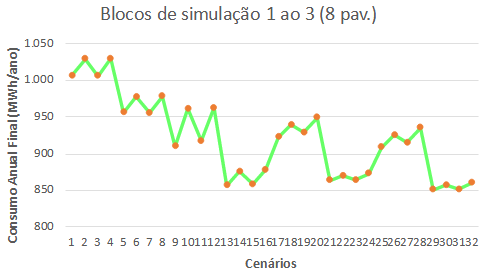
\includegraphics[width=\textwidth]{figures/result/fig25-bloco1-3.png}
    \end{subfigure}
    \begin{subfigure}[b]{0.49\textwidth}
        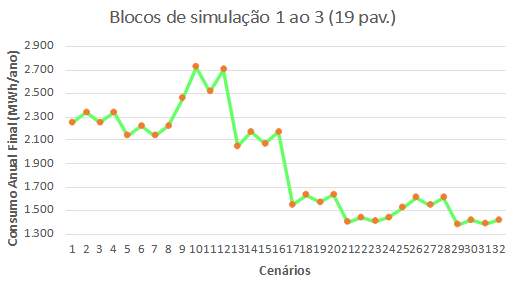
\includegraphics[width=\textwidth]{figures/result/fig26-bloco1-3.png}
    \end{subfigure}
    \begin{subfigure}[b]{0.49\textwidth}
        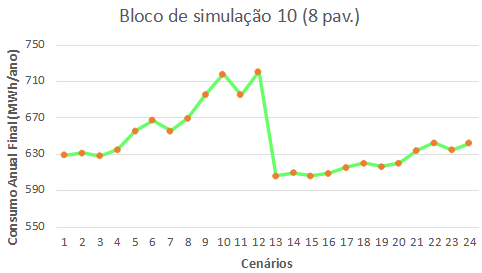
\includegraphics[width=\textwidth]{figures/result/fig27-bloco10.png}
    \end{subfigure}
    \begin{subfigure}[b]{0.49\textwidth}
        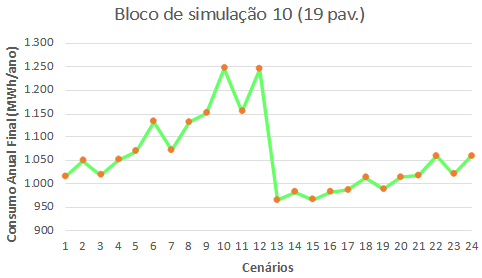
\includegraphics[width=\textwidth]{figures/result/fig28-bloco10.png}
    \end{subfigure}
    \begin{flushleft}
        \par \small Fonte: autor, (2020).
    \end{flushleft}
    \label{fig:figure25}
\end{figure}
\noindent As características das paredes e cobertura, blocos de simulação 5 e 6 respectivamente, na Figura 22, quando observadas isoladamente, são medidas importantes na redução de consumo, que neste caso representam 20\%, entre os componentes construtivos observados in loco e os componentes mais eficientes propostos para comparação. É verificada a suavização da curva de consumo entre o segundo conjunto de simulações, retratado pelos cenários 13 a 24, em relação ao primeiro conjunto, de 1 a 12, o que sinaliza a importância da envoltória e da redução da ação da radiação solar sobre os ambientes internos da edificação. A escala de consumo entre as edificações é acentuada nestes cenários, dada a semelhança do comportamento das curvas, porém, com amplitudes de 50 MW para o modelo de 8 pavimentos, e quase 200 MW para o modelo de 19 pavimentos.\vspace*{0.3cm} \newline
\noindent A influência destes componentes sobre o consumo final, junto ao vidro com baixa emissividade, atinge  o  patamar  de  26,72\%  para  a  análise  do  resultado  isolado,  como  exposto  na  Figura  \ref{fig:figure26}. Verifica-se, também, que as mudanças provocadas pela implementação das estratégias passivas, ao  longo  do  processo  de  otimização,  reduzem  a  relevância  do  vidro  com  menor  transmitância térmica para a composição construtiva e performance energética dos modelos.
\begin{figure}[H]
    \centering
    \caption{Gráficos dos blocos de simulação de paredes, 3, e coberturas, 4, dos modelos genéricos de 8 (esq.) e 19 pavimentos (dir.).}
    \begin{subfigure}[b]{0.49\textwidth}
        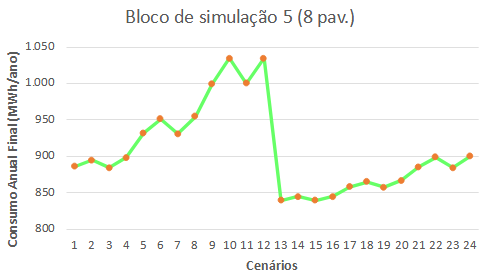
\includegraphics[width=\textwidth]{figures/result/fig29-bloco5.png}
    \end{subfigure}
    \begin{subfigure}[b]{0.49\textwidth}
        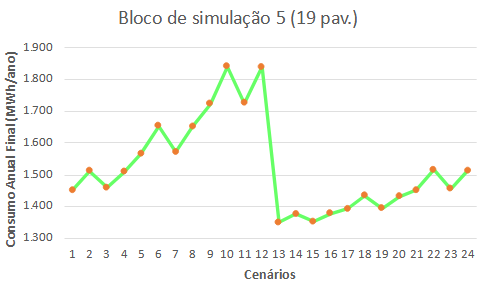
\includegraphics[width=\textwidth]{figures/result/fig30-bloco5.png}
    \end{subfigure}
    \begin{subfigure}[b]{0.49\textwidth}
        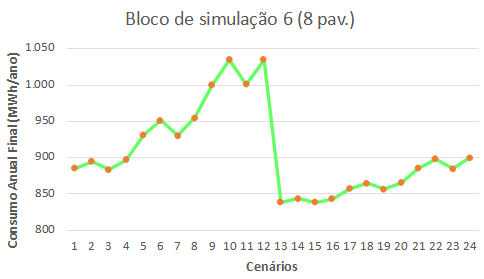
\includegraphics[width=\textwidth]{figures/result/fig31-bloco6.png}
    \end{subfigure}
    \begin{subfigure}[b]{0.49\textwidth}
        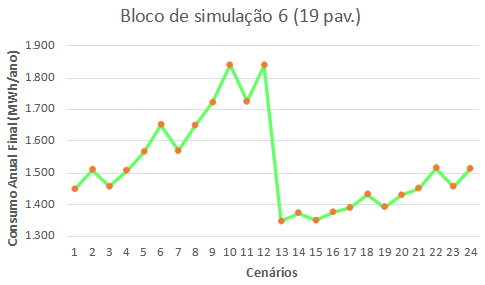
\includegraphics[width=\textwidth]{figures/result/fig32-bloco6.png}
    \end{subfigure}
    \begin{flushleft}
        \par \small Fonte: autor, (2020).
    \end{flushleft}
    \label{fig:figure26}
\end{figure}
\noindent As alterações sobre as variáveis do Percentual de Área de Abertura da Fachada Total, presentes na Figura \ref{fig:figure27}, representaram pouco impacto sobre o consumo final total quando comparado com as outras medidas implementadas. Entretanto, cabe citar que esta variável, quando observada isoladamente, corresponde a mesma grandeza de redução de consumo que as variáveis de componentes construtivos, reduzindo o consumo nos cenários simulados em cerca 18,95\% e 26,71\% para as edificações de 8 e 19 pavimentos, respectivamente. 
\begin{figure}[H]
    \centering
    \caption{Gráficos dos blocos de simulação de PAF\textsubscript{T} dos modelos genérico de 8 (esq.) e 19 pavimentos (dir.).}
    \begin{subfigure}[b]{0.49\textwidth}
        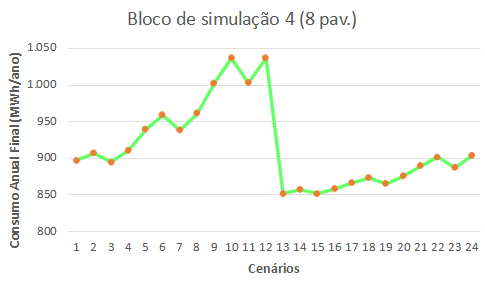
\includegraphics[width=\textwidth]{figures/result/fig33-bloco4.png}
    \end{subfigure}
    \begin{subfigure}[b]{0.49\textwidth}
        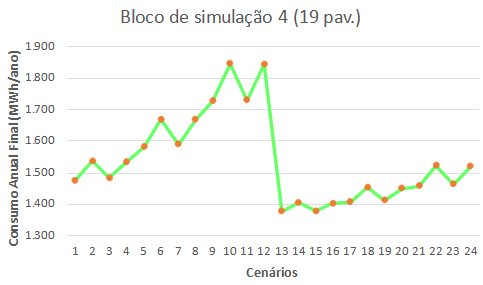
\includegraphics[width=\textwidth]{figures/result/fig34-bloco4.png}
    \end{subfigure}
    \begin{flushleft}
        \par \small Fonte: autor, (2020).
    \end{flushleft}
    \label{fig:figure27}
\end{figure}
A implementação das proteções solares, Figura \ref{fig:figure28}, apresentou redução de 6,96\% sobre o consumo total entre os blocos de simulação 5 e 6. Além desta redução, nota-se o estreitamento entre os cenários 12 e 13 neste bloco, em 23,52\%, reduzindo em 3,19\% a em relação aos blocos anteriores. Nota-se também a suavização da curva nos cenários 13 a 24 em ambas as simulações do modelo de 8 pavimentos, o que sugere a influência sobre o consumo ao controlar a quantidade de luz e de radiação no ambiente, por meio da implantação de proteções solares e de vidros mais eficientes.
\begin{figure}[H]
    \centering
    \caption{Bloco de simulações de protetores solares dos modelos genérico de 8 (esq.) e 19 pavimentos (dir.).}
    \begin{subfigure}[b]{0.49\textwidth}
        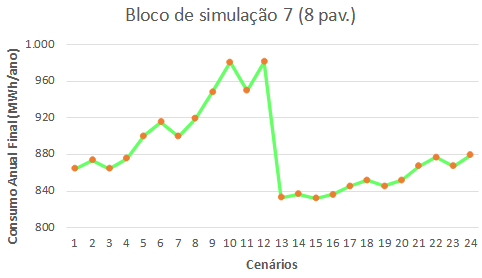
\includegraphics[width=\textwidth]{figures/result/fig35-bloco7.png}
    \end{subfigure}
    \begin{subfigure}[b]{0.49\textwidth}
        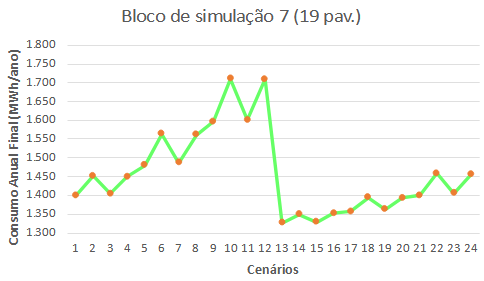
\includegraphics[width=\textwidth]{figures/result/fig36-bloco7.png}
    \end{subfigure}
    \begin{subfigure}[b]{0.49\textwidth}
        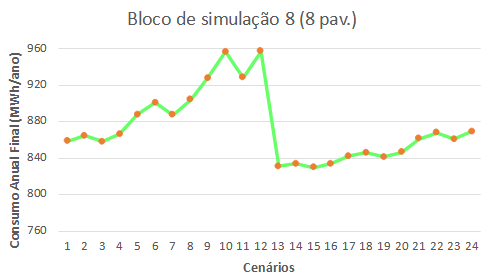
\includegraphics[width=\textwidth]{figures/result/fig37-bloco8.png}
    \end{subfigure}
    \begin{subfigure}[b]{0.49\textwidth}
        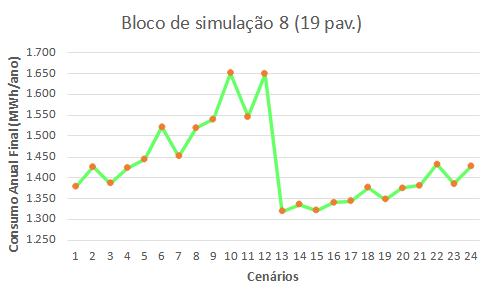
\includegraphics[width=\textwidth]{figures/result/fig38-bloco8.png}
    \end{subfigure}
    \begin{subfigure}[b]{0.49\textwidth}
        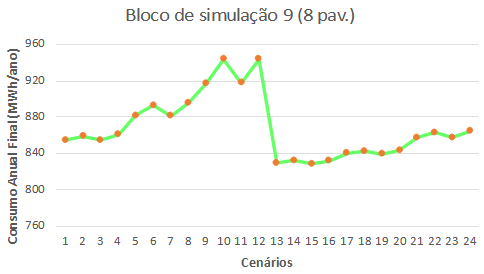
\includegraphics[width=\textwidth]{figures/result/fig39-bloco9.png}
    \end{subfigure}
    \begin{subfigure}[b]{0.49\textwidth}
        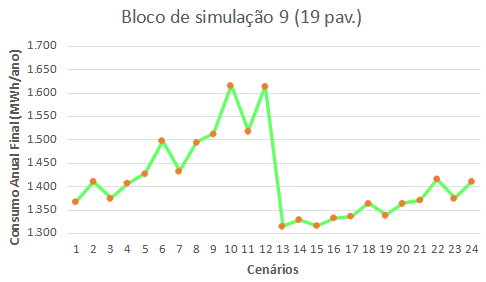
\includegraphics[width=\textwidth]{figures/result/fig40-bloco9.png}
    \end{subfigure}
    \begin{flushleft}
        \par \small Fonte: autor, (2020).
    \end{flushleft}
    \label{fig:figure28}
\end{figure}
\subsection{Geração de energia solar fotovoltaica}
\noindent Os modelos genéricos mais eficientes reduziram globalmente o consumo de energia elétrica, quando comparados com os modelos sem otimização, em cerca de 39,76\% para o modelo genérico otimizado mais eficiente, de 8 pavimentos, e 57,07\% para o modelo genérico otimizado mais eficiente, de 19 pavimentos. A partir destes resultados, foram selecionados os modelos mais eficientes entre os cenários simulados para cada tipologia e foram simuladas a implementação dos sistemas de produção de energia solar fotovoltaica.\vspace*{0.3cm} \newline
\noindent Observa-se que a energia elétrica gerada ao longo do ano, supriu a demanda de energia da edificação de 8 pavimentos para metade do ano e ligeiramente igualado em dois meses, abril e junho, como demonstrado no Gráfico 7. Anualmente, esta diferença é reduzida, produzindo maior energia do que a demanda anual, atingindo o balanço energético nulo, como apresentado no Gráfico 9. Nota-se, também, a proporção dos sistemas de condicionamento de ar – HVAC, iluminação e equipamentos em relação à produção de energia, correspondendo entre 30 a 40\% da composição do consumo para cada sistema avaliado. Os resultados com as configurações detalhadas dos equipamentos especificados estão descritos no Anexo I e II deste trabalho.
\begin{figure}[H]
    \centering
    \caption{Sistemas, consumo e produção de energia elétrica do modelo genérico de 8 pavimentos.}
    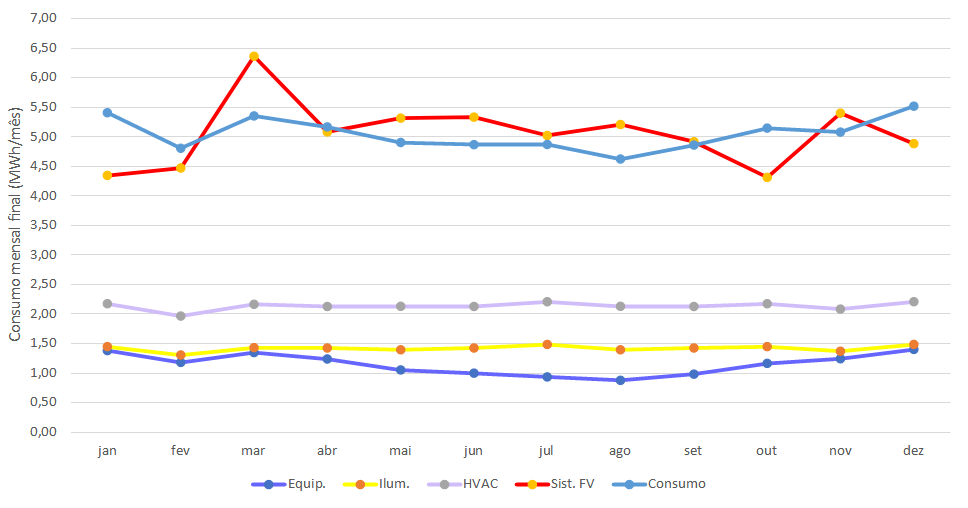
\includegraphics[width=1.0\textwidth]{figures/result/fig41-consumomod.png}
    \begin{flushleft}
        \par \small Fonte: autor, (2020).
    \end{flushleft}
    \label{fig:figure29}
\end{figure}
\noindent O desempenho do sistema de produção de energia fotovoltaica do modelo de 19 pavimentos atendeu à demanda anual. Nos meses de outubro e janeiro a demanda não foi correspondida, sendo quase nula a relação entre demanda e produção em dezembro, como observado no Gráfico 8. Observa-se que a proporção dos sistemas percebida no modelo de 8 pavimentos, em relação à produção de energia, é similarmente constatada neste modelo de 19 pavimentos.\vspace*{0.3cm} \newline
\noindent Os resultados de produção de energia para este modelo evidenciaram as características mais importantes para proporcionar maior geração de energia, como a área de fachada exposta a radiação solar e a relação entre a quantidade de pavimentos e a área de piso da edificação. Estes resultados de produção de energia em relação ao consumo foram importantes para indicar a potencialidade das edificações com dimensões como o modelo genérico proposto.
\begin{figure}[H]
    \centering
    \caption{Sistemas, consumo e produção de energia elétrica do modelo genérico de 19 pavimentos.}
    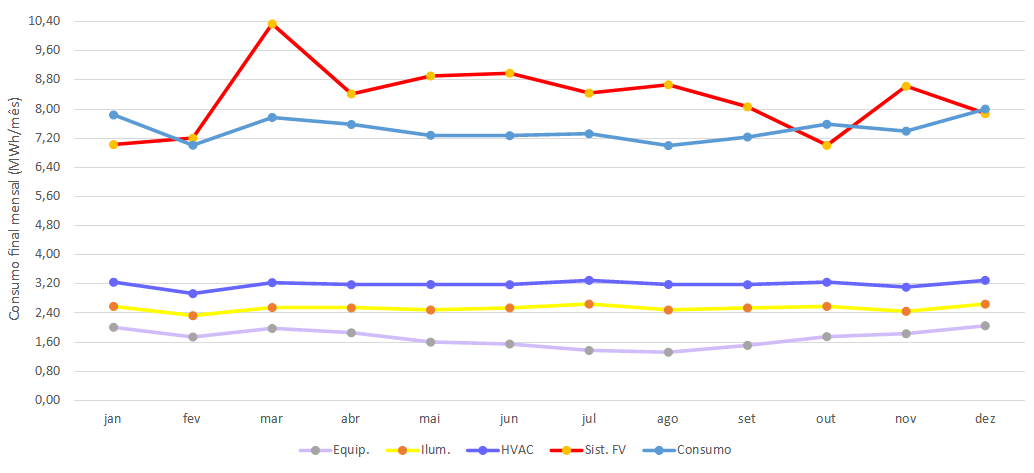
\includegraphics[width=1.0\textwidth]{figures/result/fig42-consumomod.png}
    \begin{flushleft}
        \par \small Fonte: autor, (2020).
    \end{flushleft}
    \label{fig:figure30}
\end{figure}
\vspace{-0.5cm} \noindent No Gráfico 9 e 14 são dispostas as médias mensais de consumo e produção de energia dos modelos genéricos otimizados de 8 e 19 pavimentos, respectivamente, assim como as médias anuais, as curvas tracejadas de média de produção de energia solar fotovoltaica e seus desvios padrões máximos e mínimos. Verificam-se os limites do sistema fotovoltaico para o modelo de 8 pavimentos, onde a relação quase nula entre geração e consumo de energia mensal é notada ao longo do ano simulado. Esta relação representa uma média anual de produção de energia superior ao consumo em 1,02\%, o que atesta o estado \textit{Zero Energy} para o modelo avaliado. Entretanto, a curva de desvio padrão mínimo mostra que em um cenário de pouca produção, o modelo seria dependente da energia fornecida pela concessionaria para atender as demandas mensais.\vspace{-0.3cm} 
\begin{figure}[H]
    \centering
    \caption{Consumo final mensal, Consumo vs. Produção de energia e Desvio Padrão das médias de produção de energia do modelo genérico otimizado de 8 pavimentos.}
    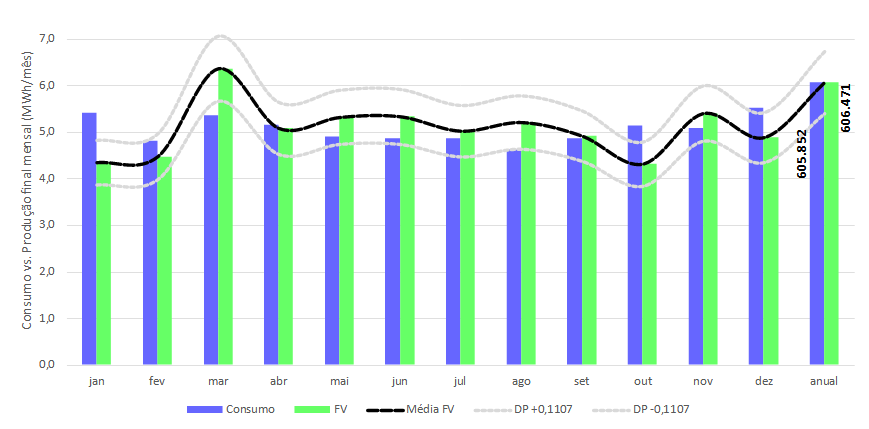
\includegraphics[width=1.0\textwidth]{figures/result/fig43-consumofinal.png}
    \begin{flushleft}
        \par \small Fonte: autor, (2020).
    \end{flushleft}
    \label{fig:figure31}
\end{figure}
\noindent Entretanto, para o cenário ótimo simulado para o modelo genérico otimizado de 19 pavimentos, percebe-se que não há a mesma dependência da Rede Pública para o fornecimento de energia. Este fato é constatado em um cenário onde a curva de desvio padrão mínimo seja a média de produção de energia do sistema sugerido, apresentando resultados superiores ao consumo na maior parte do ano.
\begin{figure}[H]
    \centering
    \caption{Consumo final mensal, Consumo vs. Produção de energia e Desvio Padrão das médias de produção de energia do modelo genérico otimizado de 19 pavimentos.}
    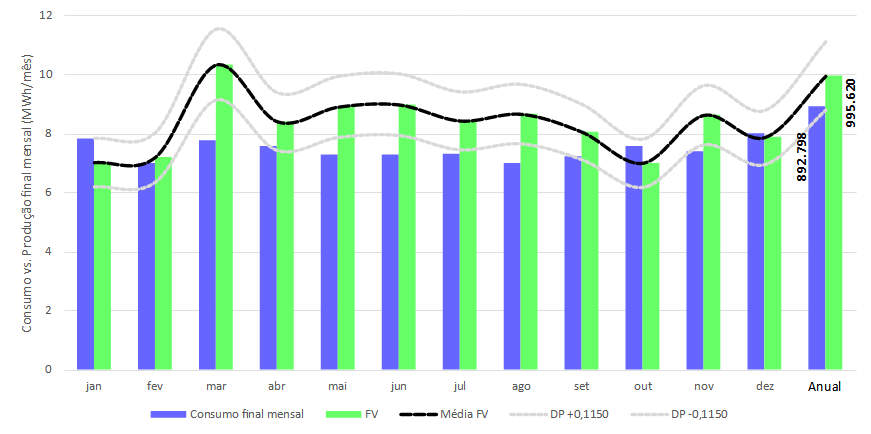
\includegraphics[width=1.0\textwidth]{figures/result/fig44-consumofinal.png}
    \begin{flushleft}
        \par \small Fonte: autor, (2020).
    \end{flushleft}
    \label{fig:figure32}
\end{figure}
\subsection{Análise de viabilidade econômica}
\noindent Os dados tarifários necessários para o cálculo de Custo Anual de Energia, CAE, foram elaborados conforme a atualização da concessionaria para o mês de janeiro de 2020. A edificação proposta é classificada como comercial e está alocada no subgrupo B3, modalidade tarifária convencional. Para o mês estudado, foi atribuído à Tarifa de Energia, TE, um acréscimo proveniente da bandeira amarela vigente. As Tarifas de Uso de Sistema de Distribuição, TUSD, e os impostos fiscais ICMS, PIS e COFINS para o período estão demonstrados na Tabela \ref{a}.
\begin{table}[H]
    \centering
    \small
    \caption{Tarifas e impostos para a modalidade tarifária convencional.}
    \begin{tabular}{ll}
    \hline
        \textbf{Tarifas e impostos}     &   \textbf{Valor}  \\\hline
        TE + Bandeira amarela           &   0,26484         \\
        TUSD                            &   0,27440         \\
        ICMS                            &   25\%            \\
        PIS+CONFINS                     &   1,57\%          \\\hline
    \end{tabular}
    \begin{flushleft}
        \par \small Fonte: autor, (2020).
    \end{flushleft}
    \label{a}
\end{table}
\noindent Para o cálculo de custo anual de energia, levou-se em consideração o consumo anual dos modelos otimizados de 8 e 19 pavimentos mais eficientes energeticamente, sendo 605.853 kWh/ano e 965.186 kWh/ano, seus respectivos consumos anuais de energia. Na Equação \ref{eq:eq11} é estabelecido o custo anual de energia sem impostos, considerando TE e TUSD.
\begin{align}\label{eq:eq11}
    &Custo_{8pav}=E_{consumida} \times (TE+TSUD)\nonumber \\
    &Custo_{8pav}=605.853 \times (0,26484+0,27440)\nonumber \\
    &Custo_{8pav}=326.700,17 \text{ reais}\nonumber \\
    &Custo_{19pav}=E_{consumida} \times (TE+TSUD)\nonumber \\
    &Custo_{19pav}=965.186 \times (0,26484+0,27440)\nonumber \\
    &Custo_{19pav}=520.166,89 \text{ reais}
\end{align}
\noindent Entretanto, os custos sofrem tributação de impostos pela distribuidora de energia, o que foi considerado para a composição real do custo anual de energia, como definido pela EDP e apresentado na Equação \ref{eq:eq12}.
\begin{align}\label{eq:eq12}
    &Custo_{8pav}=\frac{Custo_{s/imposto}}{1-(PIS+COFINS+ICMS)} \nonumber \\
    &Custo_{8pav}=\frac{326.700,17}{1-0,2675}\nonumber \\
    &Custo_{8pav}=444.913,75 \text{ reais}\nonumber \\
    &Custo_{19pav}=\frac{Custo_{s/imposto}}{1-(PIS+COFINS+ICMS)} \nonumber \\
    &Custo_{19pav}=\frac{520.166,89}{1-0,2675}\nonumber \\ 
    &Custo_{19pav}=708.384,70 \text{ reais}
\end{align}
\noindent Na Tabela \ref{tab:17} são apresentadas a quantidade de energia gerada no ano, assim como os custos dos sistemas de geração de energia solar fotovoltaica indicados, sendo que o custo de instalação por kWp dos sistemas foi orçado, em janeiro de 2020, em 784 reais para o filme fino Cd-Te \cite{Sorgato2018} e 3.682 reais para o sistema mono-Si sugerido, segundo a média de preço do mercado local.\newline
\begin{table}[H]
    \centering
    \caption{Produção de energia e custo de implantação dos sistemas fotovoltaicos.}
    \begin{tabular}{llll}
        \hline
        \multicolumn{4}{c}{\textbf{Modelo genérico de 8 pavimentos}}                                                                                                                                                                                                                \\ 
        \hline
        \textbf{Características}                                                        & \makecell[l]{\textbf{Cobertura e}\\ \textbf{estacionamento}}      & \makecell[l]{\textbf{Proteção}\\ \textbf{Solar}}          & \textbf{Fachada}                                          \\ 
        \hline
        Módulo                                                                          & \makecell[l]{SunPower \\SPR-E20-\\435-COM}                        & \makecell[l]{SunPower \\SPR-E20-\\435-COM}                & \makecell[l]{First Solar \\FS-4122-2}                     \\
        Inversor                                                                        & \makecell[l]{Fronius \\International \\IG Plus 150 V-3}           & \makecell[l]{Fronius \\International \\ECO 25.0-3-S}      & \makecell[l]{Fronius \\International \\IG Plus 150 V-3}   \\
        \makecell[l]{Energia gerada\\ (MWh/ano)}                                        & 236,40                                                            & 154,42                                                    & 215,65                                                    \\ 
        \hline
        \makecell[l]{Custo total por \\potência instalada (R\$)}                        & 552.300,00                                                        & 371.587,44                                                & 214.988,48                                                \\ 
        \hline
        \multicolumn{3}{l}{\makecell[l]{Energia total \\gerada (MWh/ano)}}                                                                                  & 606,47                                                                                                                \\
        \multicolumn{3}{l}{\makecell[l]{Custo total dos \\sistemas instalados (R\$)}}                                                                       & 1.138.875,92                                                                                                          \\ 
        \hline
        \multicolumn{4}{c}{\textbf{Modelo genérico de 19 pavimentos}}                                                                                                        \\
        \hline
        \textbf{Características}                                                        & \makecell[l]{\textbf{Cobertura e}\\ \textbf{estacionamento}}      & \textbf{Proteção Solar}                                   & \textbf{Fachada}                                          \\ 
        \hline
        Módulo                                                                          & \makecell[l]{SunPower \\SPR-E20-\\435-COM}                        & \makecell[l]{SunPower \\SPR-E20-\\435-COM}                & \makecell[l]{First Solar \\FS-4122-2}                     \\
        Inversor                                                                        & \makecell[l]{Fronius \\International \\ECO 27.0-3-S}              & \makecell[l]{Fronius \\International \\IG Plus 120 V-3}   & \makecell[l]{Fronius \\International \\IG Plus 150 V-3}   \\
        \makecell[l]{Energia gerada\\ (MWh/ano)}                                        & 236,40                                                            & 370,02                                                    & 397,12                                                    \\ 
        \hline
        \makecell[l]{Custo total por \\potência instalada (R\$)}                        & 552.300,00                                                        & 896.198,80                                                & 376.084,80                                                \\ 
        \hline
        \multicolumn{3}{l}{\makecell[l]{Energia total \\gerada (MWh/ano)}}                                                                                  & 1003,54                                                                                                               \\
        \multicolumn{3}{l}{\makecell[l]{Custo total dos \\sistemas instalados (R\$)}}                                                                       & 1.824.583,60                                                                                                          \\
        \hline
    \end{tabular}
    \begin{flushleft}
        \par \small Fonte: autor, (2020).
    \end{flushleft}
\end{table}
\noindent Os valores de retorno, V\textsubscript{r}, dos custos de implementação dos sistemas foram calculados com base na taxa de atratividade Selic de 4,5\% para o período de janeiro de 2020, representada pela incógnita i. Além disso, foram utilizados o custo anual de energia, A, e a vida útil especificada pela fabricante dos módulos utilizados, de 25 anos, representada pela incógnita \textit{n}.\newline
\begin{align}
    &V_{ret8pav}=444.913,75 \times \left\{\frac{1-\left[\frac{1}{(1+0,045)^25}\right]}{0,045}\right\} \nonumber \\
    &V_{ret8pav}=6.597.274,05 \text{ reais} \nonumber \\
    &V_{ret19pav}=708.384,70 \times \left\{\frac{1-\left[\frac{1}{(1+0,045)^25}\right]}{0,045}\right\} \nonumber \\
    &V_{ret19pav}=10.504.070,01 \text{ reais} \nonumber
\end{align}
\noindent O valor de retorno calculado dos investimentos é utilizado para estipular o valor presente, VP, de cada um dos sistemas propostos.
\begin{align}
    &V_{8pav}=6.597.274,05 - 1.138.875,92 = 5.458.398,13 \nonumber \\
    &V_{19pav}=10.504.070,01 - 1.824.583,60 = 8.679.486,41 \nonumber
\end{align}
\noindent Assim, constata-se que os sistemas de produção de energia propostos aos modelos genéricos são economicamente viáveis, visto que os VP’s são positivos. Da mesma forma, o \textit{payback} da implantação dos sistemas estudados é de 2,55 anos para o modelo de 8 pavimentos e 2,57 anos para o modelo de 19 pavimentos. Vale mencionar que as variações das taxas de energia e a perda de eficiência do sistema ao longo da vida útil não foram consideradas na avaliação de viabilidade econômica \cite{Sorgato2018}.\vspace*{0.3cm} \newline
\noindent Os resultados indicam, para o modelo de edificação adotado, a teórica viabilidade de utilização do conceito \textit{Zero Energy} para as edificações comerciais de escritório de pequeno, médio e grande porte para o recorte territorial utilizado. As condições climáticas e urbanas favoráveis, juntamente a adoção de materiais e componentes adequados ao cenário brasileiro, priorizando soluções que proporcionaram a máxima extração dos recursos energéticos on site foram essenciais para alcançar o balanço energético nulo.

%\bibliography{ref.bib}
\printbibliography

\end{document}